% Options for packages loaded elsewhere
\PassOptionsToPackage{unicode}{hyperref}
\PassOptionsToPackage{hyphens}{url}
%
\documentclass[
]{article}
\usepackage{lmodern}
\usepackage{amssymb,amsmath}
\usepackage{ifxetex,ifluatex}
\ifnum 0\ifxetex 1\fi\ifluatex 1\fi=0 % if pdftex
  \usepackage[T1]{fontenc}
  \usepackage[utf8]{inputenc}
  \usepackage{textcomp} % provide euro and other symbols
\else % if luatex or xetex
  \usepackage{unicode-math}
  \defaultfontfeatures{Scale=MatchLowercase}
  \defaultfontfeatures[\rmfamily]{Ligatures=TeX,Scale=1}
\fi
% Use upquote if available, for straight quotes in verbatim environments
\IfFileExists{upquote.sty}{\usepackage{upquote}}{}
\IfFileExists{microtype.sty}{% use microtype if available
  \usepackage[]{microtype}
  \UseMicrotypeSet[protrusion]{basicmath} % disable protrusion for tt fonts
}{}
\makeatletter
\@ifundefined{KOMAClassName}{% if non-KOMA class
  \IfFileExists{parskip.sty}{%
    \usepackage{parskip}
  }{% else
    \setlength{\parindent}{0pt}
    \setlength{\parskip}{6pt plus 2pt minus 1pt}}
}{% if KOMA class
  \KOMAoptions{parskip=half}}
\makeatother
\usepackage{xcolor}
\IfFileExists{xurl.sty}{\usepackage{xurl}}{} % add URL line breaks if available
\IfFileExists{bookmark.sty}{\usepackage{bookmark}}{\usepackage{hyperref}}
\hypersetup{
  hidelinks,
  pdfcreator={LaTeX via pandoc}}
\urlstyle{same} % disable monospaced font for URLs
\usepackage{color}
\usepackage{fancyvrb}
\newcommand{\VerbBar}{|}
\newcommand{\VERB}{\Verb[commandchars=\\\{\}]}
\DefineVerbatimEnvironment{Highlighting}{Verbatim}{commandchars=\\\{\}}
% Add ',fontsize=\small' for more characters per line
\newenvironment{Shaded}{}{}
\newcommand{\AlertTok}[1]{\textcolor[rgb]{1.00,0.00,0.00}{\textbf{#1}}}
\newcommand{\AnnotationTok}[1]{\textcolor[rgb]{0.38,0.63,0.69}{\textbf{\textit{#1}}}}
\newcommand{\AttributeTok}[1]{\textcolor[rgb]{0.49,0.56,0.16}{#1}}
\newcommand{\BaseNTok}[1]{\textcolor[rgb]{0.25,0.63,0.44}{#1}}
\newcommand{\BuiltInTok}[1]{#1}
\newcommand{\CharTok}[1]{\textcolor[rgb]{0.25,0.44,0.63}{#1}}
\newcommand{\CommentTok}[1]{\textcolor[rgb]{0.38,0.63,0.69}{\textit{#1}}}
\newcommand{\CommentVarTok}[1]{\textcolor[rgb]{0.38,0.63,0.69}{\textbf{\textit{#1}}}}
\newcommand{\ConstantTok}[1]{\textcolor[rgb]{0.53,0.00,0.00}{#1}}
\newcommand{\ControlFlowTok}[1]{\textcolor[rgb]{0.00,0.44,0.13}{\textbf{#1}}}
\newcommand{\DataTypeTok}[1]{\textcolor[rgb]{0.56,0.13,0.00}{#1}}
\newcommand{\DecValTok}[1]{\textcolor[rgb]{0.25,0.63,0.44}{#1}}
\newcommand{\DocumentationTok}[1]{\textcolor[rgb]{0.73,0.13,0.13}{\textit{#1}}}
\newcommand{\ErrorTok}[1]{\textcolor[rgb]{1.00,0.00,0.00}{\textbf{#1}}}
\newcommand{\ExtensionTok}[1]{#1}
\newcommand{\FloatTok}[1]{\textcolor[rgb]{0.25,0.63,0.44}{#1}}
\newcommand{\FunctionTok}[1]{\textcolor[rgb]{0.02,0.16,0.49}{#1}}
\newcommand{\ImportTok}[1]{#1}
\newcommand{\InformationTok}[1]{\textcolor[rgb]{0.38,0.63,0.69}{\textbf{\textit{#1}}}}
\newcommand{\KeywordTok}[1]{\textcolor[rgb]{0.00,0.44,0.13}{\textbf{#1}}}
\newcommand{\NormalTok}[1]{#1}
\newcommand{\OperatorTok}[1]{\textcolor[rgb]{0.40,0.40,0.40}{#1}}
\newcommand{\OtherTok}[1]{\textcolor[rgb]{0.00,0.44,0.13}{#1}}
\newcommand{\PreprocessorTok}[1]{\textcolor[rgb]{0.74,0.48,0.00}{#1}}
\newcommand{\RegionMarkerTok}[1]{#1}
\newcommand{\SpecialCharTok}[1]{\textcolor[rgb]{0.25,0.44,0.63}{#1}}
\newcommand{\SpecialStringTok}[1]{\textcolor[rgb]{0.73,0.40,0.53}{#1}}
\newcommand{\StringTok}[1]{\textcolor[rgb]{0.25,0.44,0.63}{#1}}
\newcommand{\VariableTok}[1]{\textcolor[rgb]{0.10,0.09,0.49}{#1}}
\newcommand{\VerbatimStringTok}[1]{\textcolor[rgb]{0.25,0.44,0.63}{#1}}
\newcommand{\WarningTok}[1]{\textcolor[rgb]{0.38,0.63,0.69}{\textbf{\textit{#1}}}}
\usepackage{graphicx}
\makeatletter
\def\maxwidth{\ifdim\Gin@nat@width>\linewidth\linewidth\else\Gin@nat@width\fi}
\def\maxheight{\ifdim\Gin@nat@height>\textheight\textheight\else\Gin@nat@height\fi}
\makeatother
% Scale images if necessary, so that they will not overflow the page
% margins by default, and it is still possible to overwrite the defaults
% using explicit options in \includegraphics[width, height, ...]{}
\setkeys{Gin}{width=\maxwidth,height=\maxheight,keepaspectratio}
% Set default figure placement to htbp
\makeatletter
\def\fps@figure{htbp}
\makeatother
\setlength{\emergencystretch}{3em} % prevent overfull lines
\providecommand{\tightlist}{%
  \setlength{\itemsep}{0pt}\setlength{\parskip}{0pt}}
\setcounter{secnumdepth}{-\maxdimen} % remove section numbering
\usepackage{pmboxdraw}
\usepackage{fontspec}
\setmonofont{Menlo}[]
\usepackage{fancyvrb}[]
\fvset{samepage=true, baselinestretch=1, frame=lines}
\renewcommand{\baselinestretch}{1.2}





\ifluatex
  \usepackage{selnolig}  % disable illegal ligatures
\fi

\author{}
\date{}

\begin{document}

\title{Exploring the uses of Quantitative Types}
\maketitle

\hypertarget{abstract}{%
\section{Abstract}\label{abstract}}

Idris2 is a programming language featuring Quantitative type
theory\cite{qtt}, a Type Theory centered around tracking \emph{usage
quantities} in addition to dependent types. This is the result of more
than 30 years of development spawned by the work of Girard on Linear
logic\cite{linear-logic}. Until Idris2, our understanding of linear
types and their uses in dependently-typed programs was hypothetical.
However this changes with languages like Idris2, which allow us to
explore the semantics of running programs using linear and dependent
types. In this thesis I explore multiple facets of programming through
the lens of quantitative programming, from ergonomics, to performance. I
will present how quantitative annotations can help the programmer write
program that precisely match their intension, help the compiler better
analyse the program written, and help the output bytecode to run faster.

\newpage
\setcounter{secnumdepth}{1}
\tableofcontents
\newpage

\hypertarget{introduction}{%
\section{Introduction}\label{introduction}}

In this project I will demonstrate different uses and results stemming
from a programming practice that allows us to specify how many times
each variable is being used. This information is part of the type
system, in our case we are tracking if a variable is allowed to be used
exactly once, or if it has no restrictions. Such types are called
``linear types''.

As we will see there is a lot more to this story, so as part of this
thesis, I will spend some time introducing dependent types and linear
types. After that we will see some examples of (new and old) uses for
linear types in Idris2. This focus on practical examples will be
followed by a context review of the existing body of theoretical work
around linear types. Once both the theoretical and practical landscape
have been set I will delve into the main two topics of this thesis, the
ergonomics of Quantitative Type Theory\(\cite{qtt}\) (QTT, for short)
for software development and the performance improvement we can derive
from the linearity features of Idris2.

The ergonomics chapter will focus on how the current implementation of
Idris can be extended, and the steps already taken toward those
extensions. The performance chapter will analyse one aspect of
performance that can be optimised thanks to clever use of linearity.

Let us begin slowly and introduce the basic concepts. The following will
only make assumptions about basic understanding of imperative and
functional programming.

\hypertarget{some-vocabulary-and-jargon}{%
\subsection{Some vocabulary and
jargon}\label{some-vocabulary-and-jargon}}

Technical papers are often hard to approach for the uninitiated because
of their heavy use of unfamiliar vocabulary and domain-specific jargon.
While jargon is useful for referencing complicated ideas succinctly, it
is a double edged sword as it also tends to hinder learning by obscuring
important concepts. Unfortunately, I do not have a solution for this
problem, but I hope this section will help mitigate this feeling of
helplessness when sentences seem to be composed of randomly generated
sequences of letters rather than legitimate words.

You will find more complete definitions at the end, in the glossary.

\hypertarget{type}{%
\subparagraph{Type}\label{type}}

A label associated to a collection of values. For example
\texttt{String} is the type given to strings of characters for text.
\texttt{Int} is the type given to integer values. \texttt{Nat} is the
type given to natural numbers.

\hypertarget{type-system}{%
\subparagraph{Type-System}\label{type-system}}

Set of rules the types in a program have to follow in order to be
accepted by the compiler. The goal of the type-system is to catch some
classes of errors while helping the programmer reach their goal more
easily.

\hypertarget{linear-types}{%
\subparagraph{Linear types}\label{linear-types}}

Types that have a usage restriction. Typically, a value labelled with a
linear type can only be used once, no less, no more.

\hypertarget{linearity-quantity-multiplicity}{%
\subparagraph{Linearity / Quantity /
Multiplicity}\label{linearity-quantity-multiplicity}}

Used interchangeably most of the time. They refer the the number of
times a variable is expected to be used.

\hypertarget{syntax}{%
\subparagraph{Syntax}\label{syntax}}

The structure of some piece of information, usual in the form of
\emph{text}. Syntax itself does not convey any meaning.

\hypertarget{semantics}{%
\subparagraph{Semantics}\label{semantics}}

The meaning associated to a piece of data, most often related to syntax.

\hypertarget{pattern-matching}{%
\subparagraph{Pattern matching}\label{pattern-matching}}

Destructuring a value into its constituent parts in order to access them
or understand what kind of value we are dealing with.

\hypertarget{generic-type-polymorphic-type-type-parameter}{%
\subparagraph{Generic type / Polymorphic type / Type
parameter}\label{generic-type-polymorphic-type-type-parameter}}

A type that needs a concrete type in order to be complete. For example
\texttt{Maybe\ a} takes the single type \texttt{a} as parameter. Once we
pass it the type \texttt{Int} it become the complete type
\texttt{Maybe\ Int}.

\hypertarget{programming-recap}{%
\subsection{Programming recap}\label{programming-recap}}

If you know about programming, you've probably heard about types and
functions. Types are ways to classify values that the computer
manipulates and functions are instructions that describe how those
values are changed.

In \emph{imperative programming} functions can perform powerful
operations like ``malloc'' and ``free'' for memory management or make
network requests through the internet. While powerful in a practical
sense, those functions are really hard to study because they are hard to
define in a mathematical way. In order to make life easier we only
consider functions in the \emph{mathematical} sense of the word : A
function is something that takes an input and returns an output.

\begin{Shaded}
\begin{Highlighting}[]
\NormalTok{f }\OperatorTok{:} \DataTypeTok{A} \OtherTok{{-}\textgreater{}} \DataTypeTok{B}
\end{Highlighting}
\end{Shaded}

This notation tells us what type the function is ready to ingest as
input and what type is expected as the output.

\begin{Shaded}
\begin{Highlighting}[]
\NormalTok{input    output}
\NormalTok{    v    v}
\NormalTok{f }\OperatorTok{:} \DataTypeTok{A} \OtherTok{{-}\textgreater{}} \DataTypeTok{B}
\OperatorTok{\^{}}
\NormalTok{name }
\end{Highlighting}
\end{Shaded}

This simplifies our model because it forbids the complexity related to
complex operations like arbitrary memory modification or network access
\footnote{We can recover those features by using patterns like ``monad''
  but it is not the topic of this brief introduction}. Functional
programming describes a programming practice centered around the use of
such functions. In addition, traditional functional programming
languages have a strong emphasis on their type system which allows the
types to describe the structure of the values very precisely.

During the rest of this thesis we are going to talk about Idris2, a
purely functional programming language featuring Quantitiative Type
Theory (QTT), a type theory\footnote{\emph{Type theory} is the abstract
  study of type systems, most often in the context of pure,
  mathematical, logic. When we say ``a Type Theory'' we mean a specific
  set of logical rules that can be implemented into a \emph{Type System}}
based around managing resources. But before we talk about QTT itself, we
have to explain what is Idris and what are dependent types.

\hypertarget{idris-and-dependent-types}{%
\subsection{Idris and dependent types}\label{idris-and-dependent-types}}

Before we jump into Idris2, allow me to introduce Idris, its
predecessor. Idris is a programming language featuring dependent types.

A way to understand dependent types is to think of the programming
language as having \emph{first class types}, that is, types are values,
just like any other, in the language. Types being normal values means we
can create them, pass them as arguments to functions and return them to
functions. This also means the difference between ``type-level'' and
``term-level'' is blurred.

\hypertarget{simple-example}{%
\subsubsection{Simple example}\label{simple-example}}

Let us start with a very simple example of a function in Idris, without
dependent types. This function returns whether or not a list \footnote{A
  list is defined as

  ``data List a = Nil \textbar{} Cons a (List a)

  Which mean a list is either empty (\texttt{Nil}) or non-empty
  (\texttt{Cons}) and will contain an element of type \texttt{a} and a
  reference to the tail of the list, which itself might be empty or not.
  It is customary to write the \texttt{Cons} case as \texttt{::}, and in
  fact the official implementation uses the symbol \texttt{::} instead
  of the word \texttt{Cons}. It is also customary to represent the empty
  list by \texttt{{[}{]}}.} is empty:

\begin{Shaded}
\begin{Highlighting}[]
\NormalTok{isEmpty }\OperatorTok{:} \DataTypeTok{List}\NormalTok{ a }\OtherTok{{-}\textgreater{}} \DataTypeTok{Bool}
\NormalTok{isEmpty [] }\OtherTok{=} \DataTypeTok{True}
\NormalTok{isEmpty (}\OtherTok{x ::}\NormalTok{ xs) }\OtherTok{=} \DataTypeTok{False}
\end{Highlighting}
\end{Shaded}

Every Idris function is comprised of two parts, the \emph{Type
signature} and the \emph{implementation} (or body) of the function. Let
us start by dissecting the Type signature:

\begin{Shaded}
\begin{Highlighting}[]
\CommentTok{{-}{-}    ┌ Name of the function}
\CommentTok{{-}{-}    │ }
\CommentTok{{-}{-}    │         ┌ Type of the argument }
\CommentTok{{-}{-}    │         │ }
\CommentTok{{-}{-}    │         │       ┌ Return type            }
\CommentTok{{-}{-} ╭──┴──╮   ╭──┴──╮  ╭─┴──╮}
\NormalTok{   isEmpty }\OperatorTok{:} \DataTypeTok{List}\NormalTok{ a }\OtherTok{{-}\textgreater{}} \DataTypeTok{Bool}
\CommentTok{{-}{-}                ▲}
\CommentTok{{-}{-}                │ }
\CommentTok{{-}{-}                └Type parameter}
\end{Highlighting}
\end{Shaded}

Every signature starts with a name, followed by a colon \texttt{:} and
ends with a type. In this case, the type is
\texttt{List\ a\ -\textgreater{}\ Bool} which represents a function that
takes a list of \texttt{a} and returns a \texttt{Bool}. Interestingly,
the type \texttt{a} is a \emph{Type parameter} and could be anything,
this function will work for all lists, irrespective of their content.

As for the body, here is how it is composed:

\begin{Shaded}
\begin{Highlighting}[]
\CommentTok{{-}{-}    ┌ Recall the function name}
\CommentTok{{-}{-}    │   }
\CommentTok{{-}{-}    │     ┌ Pattern matching on the empty list}
\CommentTok{{-}{-}    │     │   }
\CommentTok{{-}{-}    │     │    ┌ Return value}
\CommentTok{{-}{-} ╭──┴──╮  ▼  ╭─┴──╮}
\NormalTok{   isEmpty [] }\OtherTok{=} \DataTypeTok{True}
\CommentTok{{-}{-}             ┌ Pattern matching on the non{-}empty list}
\CommentTok{{-}{-}         ╭───┴───╮}
\NormalTok{   isEmpty (}\OtherTok{x ::}\NormalTok{ xs) }\OtherTok{=} \DataTypeTok{False}
\CommentTok{{-}{-}          ▲    ▲     ╰─┬─╯}
\CommentTok{{-}{-}          │    │       └ Return value}
\CommentTok{{-}{-}          │    │}
\CommentTok{{-}{-}          │    └ Tail of the list}
\CommentTok{{-}{-}          │}
\CommentTok{{-}{-}          └ Head of the list}
\end{Highlighting}
\end{Shaded}

For the body we need to recall the name of the function for every
pattern match we make. In our case we only have two cases, the empty
list \texttt{{[}{]}} and the non-empty list \texttt{x\ ::\ xs}. When we
match on a value we may discover that we can access new variables and we
give them names. In this case the \texttt{::} case allows us to bind the
head and the tail of the list to the names \texttt{x} and \texttt{xs}.
Depending on whether we are dealing with an empty list or not we return
\texttt{True} or \texttt{False} to indicate that the list is empty or
not.

Pattern matching is particularly important in Idris because it allows
the compiler to better understand how the types flow through our
program. We are going to see an example of how dependent pattern
matching manifests itself when we introduce \emph{type holes}.

\hypertarget{dependent-types-example}{%
\subsubsection{Dependent types example}\label{dependent-types-example}}

Now let us look at an example with dependent types.

\begin{Shaded}
\begin{Highlighting}[]
\NormalTok{intOrString }\OperatorTok{:}\NormalTok{ (b }\OperatorTok{:} \DataTypeTok{Bool}\NormalTok{) }\OtherTok{{-}\textgreater{}} \KeywordTok{if}\NormalTok{ b }\KeywordTok{then} \DataTypeTok{Int} \KeywordTok{else} \DataTypeTok{String}
\NormalTok{intOrString }\DataTypeTok{True} \OtherTok{=} \DecValTok{404}
\NormalTok{intOrString }\DataTypeTok{False} \OtherTok{=} \StringTok{"we got a string"}
\end{Highlighting}
\end{Shaded}

This short snippet already shows a lot of things, but again the most
important part is the type signature. Let us inspect it:

\begin{Shaded}
\begin{Highlighting}[]
\CommentTok{{-}{-}             ┌ Name of the argument}
\CommentTok{{-}{-}             │}
\CommentTok{{-}{-}             │    ┌ Type of the argument  }
\CommentTok{{-}{-}             │    │ }
\CommentTok{{-}{-}             │    │                  ┌ Return type}
\CommentTok{{-}{-}             ▼    ▼       ╭──────────┴────────────╮  }
\NormalTok{intOrString }\OperatorTok{:}\NormalTok{ (b }\OperatorTok{:} \DataTypeTok{Bool}\NormalTok{) }\OtherTok{{-}\textgreater{}} \KeywordTok{if}\NormalTok{ b }\KeywordTok{then} \DataTypeTok{Int} \KeywordTok{else} \DataTypeTok{String}
\CommentTok{{-}{-}             │               ▲}
\CommentTok{{-}{-}             └─[dependency]──┘}
\end{Highlighting}
\end{Shaded}

As you can see the return type is a \emph{program in and of itself}!
\texttt{if\ b\ then\ Int\ else\ String} returns \texttt{Int} if
\texttt{b} is \texttt{True} and \texttt{String} otherwise. Which means
the return type is different depending on the value of \texttt{b}. This
dependency is why they are called \emph{dependent types}.

\emph{Pattern matching} on the argument allows us to return different
values for each branch of our program

\begin{Shaded}
\begin{Highlighting}[]
\CommentTok{{-}{-}           ┌ \textasciigrave{}b\textasciigrave{} is True so we expect to return \textasciigrave{}Int\textasciigrave{}}
\CommentTok{{-}{-}           │}
\CommentTok{{-}{-}           │      ┌ An Int as a return value}
\CommentTok{{-}{-}           ▼    ╭─┴─╮}
\NormalTok{intOrString }\DataTypeTok{True} \OtherTok{=} \DecValTok{404} 
\NormalTok{intOrString }\DataTypeTok{False} \OtherTok{=} \StringTok{"we got a string"}
\CommentTok{{-}{-}           ▲      ╰───────┬───────╯}
\CommentTok{{-}{-}           │              └ A String as a return value}
\CommentTok{{-}{-}           │}
\CommentTok{{-}{-}           └ \textasciigrave{}b\textasciigrave{} is \textasciigrave{}False\textasciigrave{} so we expect to return a String}
\end{Highlighting}
\end{Shaded}

This typically cannot be done\footnote{Some version of dependent types
  might be achievable in other programming languages depending on how
  much the programmer is ready to indulge in arcane knowledge. But the
  core strength of Idris is that dependent types are not arcane, they
  are an integral part of the typing experience.} in programming
languages with conventional type systems. Which is why one might want to
use Idris rather than Java, C or even Haskell in order to implement
their programs.

\hypertarget{holes-in-idris}{%
\subsubsection{Holes in Idris}\label{holes-in-idris}}

A very useful feature of Idris is \emph{type holes}, one can replace any
term by a variable name prefixed by a question mark, like this :
\texttt{?hole} . This tells the compiler to infer the type at this
position and report it to the user in order to better understand what
value could possibly fit the expected type. In addition, the compiler
will also report what it knows about the surrounding context to give
additional insight.

If we take our example of \texttt{intOrString} and replace the
implementation by a hole we have the following:

\begin{Shaded}
\begin{Highlighting}[]
\NormalTok{intOrString }\OperatorTok{:}\NormalTok{ (b }\OperatorTok{:} \DataTypeTok{Bool}\NormalTok{) }\OtherTok{{-}\textgreater{}} \KeywordTok{if}\NormalTok{ b }\KeywordTok{then} \DataTypeTok{Int} \KeywordTok{else} \DataTypeTok{String}
\NormalTok{intOrString b }\OtherTok{=} \OperatorTok{?}\NormalTok{hole}
\end{Highlighting}
\end{Shaded}

We can then ask the compiler what is the expected type, information
provided by the compiler will be shown with a column of
\texttt{\textgreater{}} on the left side to distinguish it from code.
Here is the type we get when asking about our \texttt{hole}:

\begin{Shaded}
\begin{Highlighting}[]
\OperatorTok{\textgreater{}}\NormalTok{ b }\OperatorTok{:} \DataTypeTok{Bool}
\OperatorTok{\textgreater{}} \CommentTok{{-}{-}{-}{-}{-}{-}{-}{-}{-}{-}{-}{-}{-}{-}{-}{-}{-}{-}{-}{-}{-}{-}{-}{-}{-}{-}{-}{-}{-}{-}{-}{-}}
\OperatorTok{\textgreater{}}\NormalTok{ hole }\OperatorTok{:} \KeywordTok{if}\NormalTok{ b }\KeywordTok{then} \DataTypeTok{Int} \KeywordTok{else} \DataTypeTok{String}
\end{Highlighting}
\end{Shaded}

This information does not tell us what value we can use. However it
informs us that the type of the value \emph{depends on the value of
\texttt{b}} . Therefore, pattern matching \footnote{Idris has an
  interactive mode that allows the pattern matching to be done
  automatically by hitting a simple key stroke which will generate the
  code in the snippet automatically. This won't be showcased here, as it
  is not an Idris development tutorial, but one can read more about it
  in \emph{Type Driven Development in Idris} by Edwin Brady.} on
\texttt{b} might give us more insight.

\begin{Shaded}
\begin{Highlighting}[]
\NormalTok{intOrString }\OperatorTok{:}\NormalTok{ (b }\OperatorTok{:} \DataTypeTok{Bool}\NormalTok{) }\OtherTok{{-}\textgreater{}} \KeywordTok{if}\NormalTok{ b }\KeywordTok{then} \DataTypeTok{Int} \KeywordTok{else} \DataTypeTok{String}
\NormalTok{intOrString }\DataTypeTok{True} \OtherTok{=} \OperatorTok{?}\NormalTok{hole1}
\NormalTok{intOrString }\DataTypeTok{False} \OtherTok{=} \OperatorTok{?}\NormalTok{hole2}
\end{Highlighting}
\end{Shaded}

Asking again what is in \texttt{hole1} gets us

\begin{Shaded}
\begin{Highlighting}[]
\OperatorTok{\textgreater{}}\NormalTok{ hole1 }\OperatorTok{:} \DataTypeTok{Int}
\end{Highlighting}
\end{Shaded}

and \texttt{hole2} gets us

\begin{Shaded}
\begin{Highlighting}[]
\OperatorTok{\textgreater{}}\NormalTok{ hole2 }\OperatorTok{:} \DataTypeTok{String}
\end{Highlighting}
\end{Shaded}

Which we can fill with literal values like \texttt{123} or
\texttt{"good\ afternoon"}. The complete program would look like this:

\begin{Shaded}
\begin{Highlighting}[]
\NormalTok{intOrString }\OperatorTok{:}\NormalTok{ (b }\OperatorTok{:} \DataTypeTok{Bool}\NormalTok{) }\OtherTok{{-}\textgreater{}} \KeywordTok{if}\NormalTok{ b }\KeywordTok{then} \DataTypeTok{Int} \KeywordTok{else} \DataTypeTok{String}
\NormalTok{intOrString }\DataTypeTok{True} \OtherTok{=} \DecValTok{123}
\NormalTok{intOrString }\DataTypeTok{False} \OtherTok{=} \StringTok{"good afternoon"}
\end{Highlighting}
\end{Shaded}

\hypertarget{whats-wrong-with-non-dependent-types}{%
\subsubsection{What's wrong with non-dependent
types?}\label{whats-wrong-with-non-dependent-types}}

Non-dependent type systems cannot represent the behaviour described by
\texttt{intOrString} and have to resort to patterns like \texttt{Either}
\footnote{Defined as : ``data Either a b = Left a \textbar{} Right b} to
encapsulate the two possible cases our program can encounter.

\begin{Shaded}
\begin{Highlighting}[]
\OtherTok{eitherIntOrString ::} \DataTypeTok{Bool} \OtherTok{{-}\textgreater{}} \DataTypeTok{Either} \DataTypeTok{Int} \DataTypeTok{String}
\NormalTok{eitherIntOrString }\DataTypeTok{True} \OtherTok{=} \DataTypeTok{Left} \DecValTok{404}
\NormalTok{eitherIntOrString }\DataTypeTok{False} \OtherTok{=} \DataTypeTok{Right} \StringTok{"we got a string"}
\end{Highlighting}
\end{Shaded}

While this is fine in principle, it comes with a set of drawbacks that
cannot be solved without dependent types. In order to see this, let us
place a hole in the implementation of \texttt{eitherIntOrString}:

\begin{Shaded}
\begin{Highlighting}[]
\NormalTok{eitherIntOrString }\OperatorTok{:} \DataTypeTok{Bool} \OtherTok{{-}\textgreater{}} \DataTypeTok{Either} \DataTypeTok{Int} \DataTypeTok{String}
\NormalTok{eitherIntOrString b }\OtherTok{=} \OperatorTok{?}\NormalTok{hole}
\end{Highlighting}
\end{Shaded}

\begin{Shaded}
\begin{Highlighting}[]
\OperatorTok{\textgreater{}}\NormalTok{ b }\OperatorTok{:} \DataTypeTok{Bool}
\OperatorTok{\textgreater{}} \CommentTok{{-}{-}{-}{-}{-}{-}{-}{-}{-}{-}{-}{-}{-}{-}{-}{-}{-}{-}{-}{-}{-}{-}{-}{-}}
\OperatorTok{\textgreater{}}\NormalTok{ hole }\OperatorTok{:} \DataTypeTok{Either} \DataTypeTok{Int} \DataTypeTok{String}
\end{Highlighting}
\end{Shaded}

While this type might be easier to read than
\texttt{if\ b\ then\ Int\ else\ String} it does not tell us how to
proceed in order to find a more precise type to fill. We can try pattern
matching on \texttt{b}:

\begin{Shaded}
\begin{Highlighting}[]
\NormalTok{intOrString\textquotesingle{} }\OperatorTok{:} \DataTypeTok{Bool} \OtherTok{{-}\textgreater{}} \DataTypeTok{Either} \DataTypeTok{Int} \DataTypeTok{String}
\NormalTok{intOrString\textquotesingle{} }\DataTypeTok{True} \OtherTok{=} \OperatorTok{?}\NormalTok{hole1}
\NormalTok{intOrString\textquotesingle{} }\DataTypeTok{False} \OtherTok{=} \OperatorTok{?}\NormalTok{hole2}
\end{Highlighting}
\end{Shaded}

But it does not provide any additional information about the return
types to use.

\begin{Shaded}
\begin{Highlighting}[]
\OperatorTok{\textgreater{}} \CommentTok{{-}{-}{-}{-}{-}{-}{-}{-}{-}{-}{-}}
\OperatorTok{\textgreater{}}\NormalTok{ hole1 }\OperatorTok{:} \DataTypeTok{Either} \DataTypeTok{Int} \DataTypeTok{String}
\end{Highlighting}
\end{Shaded}

\begin{Shaded}
\begin{Highlighting}[]
\OperatorTok{\textgreater{}} \CommentTok{{-}{-}{-}{-}{-}{-}{-}{-}{-}{-}{-}}
\OperatorTok{\textgreater{}}\NormalTok{ hole2 }\OperatorTok{:} \DataTypeTok{Either} \DataTypeTok{Int} \DataTypeTok{String}
\end{Highlighting}
\end{Shaded}

In itself using \texttt{Either} isn't a problem, however
\texttt{Either}'s lack of information manifests itself in other ways
during programming; take the following program:

\begin{Shaded}
\begin{Highlighting}[]
\NormalTok{checkType }\OperatorTok{:} \DataTypeTok{Int}
\NormalTok{checkType }\OtherTok{=} \KeywordTok{let}\NormalTok{ intValue }\OtherTok{=}\NormalTok{ eitherIntOrString }\DataTypeTok{True} \KeywordTok{in} \OperatorTok{?}\NormalTok{hole}
\end{Highlighting}
\end{Shaded}

\begin{Shaded}
\begin{Highlighting}[]
\OperatorTok{\textgreater{}}\NormalTok{ intValue }\OperatorTok{:} \DataTypeTok{Either} \DataTypeTok{Int} \DataTypeTok{String}
\OperatorTok{\textgreater{}} \CommentTok{{-}{-}{-}{-}{-}{-}{-}{-}{-}{-}{-}{-}{-}{-}{-}}
\OperatorTok{\textgreater{}}\NormalTok{ hole }\OperatorTok{:} \DataTypeTok{Int}
\end{Highlighting}
\end{Shaded}

The compiler is unable to tell us if this value is an \texttt{Int} or a
\texttt{String}. Despite us \emph{knowing} that \texttt{IntOrString}
returns an \texttt{Int} when passed \texttt{True}, we cannot use this
fact to convince the compiler to simplify the type for us. We have to go
through a runtime check to ensure that the value we are inspecting is
indeed an \texttt{Int}:

\begin{Shaded}
\begin{Highlighting}[]
\NormalTok{checkType }\OperatorTok{:} \DataTypeTok{Int}
\NormalTok{checkType }\OtherTok{=} \KeywordTok{let}\NormalTok{ intValue }\OtherTok{=}\NormalTok{ eitherIntOrString }\DataTypeTok{True} \KeywordTok{in}
                \KeywordTok{case}\NormalTok{ intValue }\KeywordTok{of}
\NormalTok{                     (}\DataTypeTok{Left}\NormalTok{ i) }\OtherTok{=\textgreater{}} \OperatorTok{?}\NormalTok{hole1}
\NormalTok{                     (}\DataTypeTok{Right}\NormalTok{ str) }\OtherTok{=\textgreater{}} \OperatorTok{?}\NormalTok{hole2}
\end{Highlighting}
\end{Shaded}

But doing so introduces the additional problem that we now need to
provide a value for an impossible case (\texttt{Right}). What do we even
return? We do not have an \texttt{Int} at hand to use. Our alternatives
are:

\begin{itemize}
\tightlist
\item
  Panic and crash the program.
\item
  Make up a default value, silencing the error but hiding a potential
  bug.
\item
  Change the return type to \texttt{Either\ Int\ String} and letting the
  caller deal with it.
\end{itemize}

None of which are ideal nor replicate the functionality of the dependent
version we saw before. This is why dependent types are desirable, they
help: - Avoid needless runtime checks. - The compiler better understand
the semantics of the program. - Inform the programmer by communicating
precisely which types are expected.

This concludes our short introduction to dependent types and I hope
you've been convinced of their usefulness. In the next section we are
going to talk about linear types.

\hypertarget{idris2-and-linear-types}{%
\subsection{Idris2 and linear types}\label{idris2-and-linear-types}}

Idris2 takes things further and introduces \emph{linear types} in its
type system, allowing us to define how many times a variable will be
used. Three different quantities exist in Idris2 : \texttt{0},
\texttt{1} and \texttt{ω}. \texttt{0} means the value cannot be used in
the body of a function, \texttt{1} means it has to be used exactly once,
no less, no more. \texttt{ω} means the variable isn't subject to any
usage restrictions, just like other (non-linear) programming languages.

We are going to revisit this concept later as there are more subtleties,
especially about the \texttt{0} usage. For now we are going to explore
some examples of linear functions and linear types, starting with very
simple functions such as incrementing numbers.

\hypertarget{incremental-steps}{%
\subsubsection{Incremental steps}\label{incremental-steps}}

When designing examples, natural numbers are a straightforward data type
to turn to. Their definition is extremely simple:
\texttt{data\ Nat\ =\ Z\ \textbar{}\ S\ Nat} which means that a
\texttt{Nat} is either zero \texttt{Z} or the successor of another
natural number, \texttt{S}.

Given this definition let us look at the function that increments a
natural number:

\begin{Shaded}
\begin{Highlighting}[]
\NormalTok{increment }\OperatorTok{:} \DataTypeTok{Nat} \OtherTok{{-}\textgreater{}} \DataTypeTok{Nat}
\NormalTok{increment n }\OtherTok{=} \DataTypeTok{S}\NormalTok{ n}
\end{Highlighting}
\end{Shaded}

As we've seen before with our \texttt{intOrString} function we can name
our arguments in order to refer to them later in the type signature. We
can do the same here even if we do not use the argument in a dependent
type. Here we are going to name our first argument \texttt{n}.

\begin{Shaded}
\begin{Highlighting}[]
\NormalTok{increment }\OperatorTok{:}\NormalTok{ (n }\OperatorTok{:} \DataTypeTok{Nat}\NormalTok{) }\OtherTok{{-}\textgreater{}} \DataTypeTok{Nat}
\NormalTok{increment n }\OtherTok{=} \DataTypeTok{S}\NormalTok{ n}
\end{Highlighting}
\end{Shaded}

In this case, the name \texttt{n} doesn't serve any other purpose than
documentation, but our implementation of linear types has one
particularity: quantities have to be assigned to a \emph{name}
(something we will explore in further details in a later section). Since
the argument of \texttt{increment} is used exactly once in the body of
the function we can update our type signature to assign the quantity
\texttt{1} to the argument \texttt{n}

\begin{Shaded}
\begin{Highlighting}[]
\CommentTok{{-}{-}           ┌ We declare \textasciigrave{}n\textasciigrave{} to be linear}
\CommentTok{{-}{-}           ▼}
\NormalTok{increment }\OperatorTok{:}\NormalTok{ (}\DecValTok{1}\NormalTok{ n }\OperatorTok{:} \DataTypeTok{Nat}\NormalTok{) }\OtherTok{{-}\textgreater{}} \DataTypeTok{Nat}
\NormalTok{increment n }\OtherTok{=} \DataTypeTok{S}\NormalTok{ n}
\CommentTok{{-}{-}              ▲}
\CommentTok{{-}{-}              │}
\CommentTok{{-}{-}              └ We use n once here}
\end{Highlighting}
\end{Shaded}

Additionally, Idris2 feature pattern matching and the rules of linearity
also apply to each variable that was bound when matching on it. That is,
if the value we are matching is linear then we need to use the pattern
variables linearly.

\begin{Shaded}
\begin{Highlighting}[]
\FunctionTok{sum} \OperatorTok{:}\NormalTok{ (}\DecValTok{1}\NormalTok{ n }\OperatorTok{:} \DataTypeTok{Nat}\NormalTok{) }\OtherTok{{-}\textgreater{}}\NormalTok{ (}\DecValTok{1}\NormalTok{ m }\OperatorTok{:} \DataTypeTok{Nat}\NormalTok{) }\OtherTok{{-}\textgreater{}} \DataTypeTok{Nat}
\FunctionTok{sum} \DataTypeTok{Z}\NormalTok{ m }\OtherTok{=}\NormalTok{ m}
\CommentTok{{-}{-}  ▲}
\CommentTok{{-}{-}  └ We match on the argument here}
\FunctionTok{sum}\NormalTok{ (}\DataTypeTok{S}\NormalTok{ n) m }\OtherTok{=} \DataTypeTok{S}\NormalTok{ (}\FunctionTok{sum}\NormalTok{ n m)}
\CommentTok{{-}{-}  ╰─┬─╯            ▲}
\CommentTok{{-}{-}    │              └ We use \textasciigrave{}n\textasciigrave{}}
\CommentTok{{-}{-}    │}
\CommentTok{{-}{-}    └ We match on the argument and bind \textasciigrave{}n\textasciigrave{}}
\end{Highlighting}
\end{Shaded}

In this last example we match on \texttt{S} and bind the argument of
\texttt{S} to the variable \texttt{n}. Since the original argument was
linear, \texttt{n} is linear too and is indeed used later with
\texttt{sum\ n\ m}.

\hypertarget{dropping-and-picking-it-up-again}{%
\subsubsection{Dropping and picking it up
again}\label{dropping-and-picking-it-up-again}}

Obviously this programming discipline does not allow us to express every
program the same way as before. Here are two typical examples that
cannot be expressed :

\begin{Shaded}
\begin{Highlighting}[]
\FunctionTok{drop} \OperatorTok{:}\NormalTok{ (}\DecValTok{1}\NormalTok{ v }\OperatorTok{:}\NormalTok{ a) }\OtherTok{{-}\textgreater{}}\NormalTok{ ()}

\NormalTok{copy }\OperatorTok{:}\NormalTok{ (}\DecValTok{1}\NormalTok{ v }\OperatorTok{:}\NormalTok{ a) }\OtherTok{{-}\textgreater{}}\NormalTok{ (a, a)}
\end{Highlighting}
\end{Shaded}

We can explore what is wrong with those functions by trying to implement
them and making use of holes.

\begin{Shaded}
\begin{Highlighting}[]
\FunctionTok{drop} \OperatorTok{:}\NormalTok{ (}\DecValTok{1}\NormalTok{ v }\OperatorTok{:}\NormalTok{ a) }\OtherTok{{-}\textgreater{}}\NormalTok{ ()}
\FunctionTok{drop}\NormalTok{ v }\OtherTok{=} \OperatorTok{?}\NormalTok{drop\_rhs}
\end{Highlighting}
\end{Shaded}

\begin{Shaded}
\begin{Highlighting}[]
\OperatorTok{\textgreater{}} \DecValTok{0}\NormalTok{ a }\OperatorTok{:} \DataTypeTok{Type}
\OperatorTok{\textgreater{}} \DecValTok{1}\NormalTok{ v }\OperatorTok{:}\NormalTok{ a}
\OperatorTok{\textgreater{}} \CommentTok{{-}{-}{-}{-}{-}{-}{-}{-}{-}{-}{-}{-}}
\OperatorTok{\textgreater{}}\NormalTok{ drop\_rhs }\OperatorTok{:}\NormalTok{ ()}
\end{Highlighting}
\end{Shaded}

As you can see, each variable is annotated with an additional number on
its left, \texttt{0} or \texttt{1}, that informs us how many times each
variable has to be used (If there is no restriction, the usage number is
simply left blank, just like our previous examples didn't show any usage
numbers).

As you can see we need to use \texttt{v} (since it marked with
\texttt{1}) but we are only allowed to return \texttt{()}. This would be
solved if we had a function of type
\texttt{(1\ v\ :\ a)\ -\textgreater{}\ ()} to consume the value and
return \texttt{()}, but this is exactly the signature of the function we
are trying to implement!

If we try to implement the function by returning \texttt{()} directly we
get the following:

\begin{Shaded}
\begin{Highlighting}[]
\FunctionTok{drop} \OperatorTok{:}\NormalTok{ (}\DecValTok{1}\NormalTok{ v }\OperatorTok{:}\NormalTok{ a) }\OtherTok{{-}\textgreater{}}\NormalTok{ ()}
\FunctionTok{drop}\NormalTok{ v }\OtherTok{=}\NormalTok{ ()}
\end{Highlighting}
\end{Shaded}

\begin{Shaded}
\begin{Highlighting}[]
\OperatorTok{\textgreater{}} \DataTypeTok{There}\NormalTok{ are }\DecValTok{0}\NormalTok{ uses }\KeywordTok{of}\NormalTok{ linear variable v}
\end{Highlighting}
\end{Shaded}

Which indicates that \texttt{v} is supposed to be used but no uses have
been found.

Similarly for \texttt{copy} we have

\begin{Shaded}
\begin{Highlighting}[]
\NormalTok{copy }\OperatorTok{:}\NormalTok{ (}\DecValTok{1}\NormalTok{ v }\OperatorTok{:}\NormalTok{ a) }\OtherTok{{-}\textgreater{}}\NormalTok{ (a, a)}
\NormalTok{copy v }\OtherTok{=} \OperatorTok{?}\NormalTok{hole}
\end{Highlighting}
\end{Shaded}

\begin{Shaded}
\begin{Highlighting}[]
\OperatorTok{\textgreater{}} \DecValTok{0}\NormalTok{ a }\OperatorTok{:} \DataTypeTok{Type}
\OperatorTok{\textgreater{}} \DecValTok{1}\NormalTok{ v }\OperatorTok{:}\NormalTok{ a}
\OperatorTok{\textgreater{}} \CommentTok{{-}{-}{-}{-}{-}{-}{-}{-}{-}{-}{-}}
\OperatorTok{\textgreater{}}\NormalTok{ hole }\OperatorTok{:}\NormalTok{ (a, a)}
\end{Highlighting}
\end{Shaded}

In which we need to use \texttt{v} twice but we're only allow to use it
once. Using it twice result in this program with this error

\begin{Shaded}
\begin{Highlighting}[]
\NormalTok{copy }\OperatorTok{:}\NormalTok{ (}\DecValTok{1}\NormalTok{ v }\OperatorTok{:}\NormalTok{ a) }\OtherTok{{-}\textgreater{}}\NormalTok{ (a, a)}
\NormalTok{copy v }\OtherTok{=}\NormalTok{ (v, v)}
\end{Highlighting}
\end{Shaded}

\begin{Shaded}
\begin{Highlighting}[]
\OperatorTok{\textgreater{}} \DataTypeTok{There}\NormalTok{ are }\DecValTok{2}\NormalTok{ uses }\KeywordTok{of}\NormalTok{ linear variable v}
\end{Highlighting}
\end{Shaded}

Interestingly enough, partially implementing our program with a hole
gives us an amazing insight

\begin{Shaded}
\begin{Highlighting}[]
\NormalTok{copy }\OperatorTok{:}\NormalTok{ (}\DecValTok{1}\NormalTok{ v }\OperatorTok{:}\NormalTok{ a) }\OtherTok{{-}\textgreater{}}\NormalTok{ (a, a)}
\NormalTok{copy v }\OtherTok{=}\NormalTok{ (v, }\OperatorTok{?}\NormalTok{hole)}
\end{Highlighting}
\end{Shaded}

\begin{Shaded}
\begin{Highlighting}[]
\OperatorTok{\textgreater{}} \DecValTok{0}\NormalTok{ a }\OperatorTok{:} \DataTypeTok{Type}
\OperatorTok{\textgreater{}} \DecValTok{0}\NormalTok{ v }\OperatorTok{:}\NormalTok{ a}
\OperatorTok{\textgreater{}} \CommentTok{{-}{-}{-}{-}{-}{-}{-}{-}{-}{-}{-}}
\OperatorTok{\textgreater{}}\NormalTok{ hole }\OperatorTok{:}\NormalTok{ a}
\end{Highlighting}
\end{Shaded}

The hole has been updated to reflect the fact that though \texttt{v} is
in scope, no uses of it are available. Despite that we still need to
make up a value of type \texttt{a} out of thin air, which is impossible
\footnote{This is because we have no information about the type
  parameter \texttt{a}, as we will see later, if we are given more
  information about how to construct and destructure values, we
  \emph{can} implement \texttt{copy} and \texttt{drop}.}.

While there are experimental ideas that allow us to recover those
capabilities they are not currently present in Idris2. We will talk
about those limitations and how to overcome them in the ``limitations
and solutions for quantitative types'' section.

\hypertarget{dancing-around-linear-types}{%
\subsubsection{Dancing around linear
types}\label{dancing-around-linear-types}}

Linear values cannot be duplicated or ignored, but provided we know how
the values are constructed, we can work hard enough to tear them apart
and build them back up. This allows us to dance around the issue of
ignoring and duplicating linear variables by exploiting pattern matching
in order to implement functions such as
\texttt{copy\ :\ (1\ \_\ :\ a)\ \textasciigrave{}-\textgreater{}\ (a,\ a)}
and \texttt{drop\ :\ (1\ \_\ :\ a)\ -\textgreater{}\ ()}

The next snippet show how to implement those for \texttt{Nat}:

\begin{Shaded}
\begin{Highlighting}[]
\NormalTok{dropNat }\OperatorTok{:}\NormalTok{ (}\DecValTok{1}\NormalTok{ \_ }\OperatorTok{:} \DataTypeTok{Nat}\NormalTok{) }\OtherTok{{-}\textgreater{}}\NormalTok{ ()}
\NormalTok{dropNat }\DataTypeTok{Z} \OtherTok{=}\NormalTok{ ()}
\NormalTok{dropNat (}\DataTypeTok{S}\NormalTok{ n) }\OtherTok{=}\NormalTok{ dropNat n}

\NormalTok{copyNat }\OperatorTok{:}\NormalTok{ (}\DecValTok{1}\NormalTok{ \_ }\OperatorTok{:} \DataTypeTok{Nat}\NormalTok{) }\OtherTok{{-}\textgreater{}}\NormalTok{ (}\DataTypeTok{Nat}\NormalTok{, }\DataTypeTok{Nat}\NormalTok{)}
\NormalTok{copyNat }\DataTypeTok{Z} \OtherTok{=}\NormalTok{ (}\DataTypeTok{Z}\NormalTok{, }\DataTypeTok{Z}\NormalTok{)}
\NormalTok{copyNat (}\DataTypeTok{S}\NormalTok{ n) }\OtherTok{=} \KeywordTok{let}\NormalTok{ (a, b) }\OtherTok{=}\NormalTok{ copyNat n }\KeywordTok{in}
\NormalTok{                    (}\DataTypeTok{S}\NormalTok{ a, }\DataTypeTok{S}\NormalTok{ b)}
\end{Highlighting}
\end{Shaded}

It is worth noticing that \texttt{dropNat} effectively spends
\texttt{O(n)} doing nothing, while \texttt{copyNat} \emph{simulates}
allocation by constructing a new value that is identical and takes the
same space as the original one (albeit very inefficiently, one would
expect a \texttt{memcpy} to be \texttt{O(1)}, not \texttt{O(n)} in the
size of the input).

We can encapsulate those functions in the following interfaces:

\begin{Shaded}
\begin{Highlighting}[]
\NormalTok{interface }\DataTypeTok{Drop}\NormalTok{ a }\KeywordTok{where}
    \FunctionTok{drop} \OperatorTok{:}\NormalTok{ (}\DecValTok{1}\NormalTok{ \_ }\OperatorTok{:}\NormalTok{ a) }\OtherTok{{-}\textgreater{}}\NormalTok{ ()}

\NormalTok{interface }\DataTypeTok{Copy}\NormalTok{ a }\KeywordTok{where}
\NormalTok{    copy }\OperatorTok{:}\NormalTok{ (}\DecValTok{1}\NormalTok{ \_ }\OperatorTok{:}\NormalTok{ a) }\OtherTok{{-}\textgreater{}}\NormalTok{ (a, a)}
\end{Highlighting}
\end{Shaded}

Since we know how to implement those for \texttt{Nat} we can ask
ourselves how we could give implementation of those interfaces to
additional types.

\begin{Shaded}
\begin{Highlighting}[]
\KeywordTok{module} \DataTypeTok{Main}

\KeywordTok{import} \DataTypeTok{Data.List}

\KeywordTok{data} \DataTypeTok{Tree}\NormalTok{ a }\OtherTok{=} \DataTypeTok{Leaf}\NormalTok{ a }\OperatorTok{|} \DataTypeTok{Branch}\NormalTok{ a (}\DataTypeTok{Tree}\NormalTok{ a) (}\DataTypeTok{Tree}\NormalTok{ a)}

\NormalTok{interface }\DataTypeTok{Drop}\NormalTok{ a }\KeywordTok{where}
    \FunctionTok{drop} \OperatorTok{:}\NormalTok{ (}\DecValTok{1}\NormalTok{ \_ }\OperatorTok{:}\NormalTok{ a) }\OtherTok{{-}\textgreater{}}\NormalTok{ ()}

\NormalTok{interface }\DataTypeTok{Copy}\NormalTok{ a }\KeywordTok{where}
\NormalTok{    copy }\OperatorTok{:}\NormalTok{ (}\DecValTok{1}\NormalTok{ \_ }\OperatorTok{:}\NormalTok{ a) }\OtherTok{{-}\textgreater{}}\NormalTok{ (a, a)}

\DataTypeTok{Drop}\NormalTok{ a }\OtherTok{=\textgreater{}} \DataTypeTok{Drop}\NormalTok{ (}\DataTypeTok{List}\NormalTok{ a) }\KeywordTok{where}
\NormalTok{    copy ls }\OtherTok{=} \OperatorTok{?}\NormalTok{drop\_list\_impl}

\DataTypeTok{Copy}\NormalTok{ a }\OtherTok{=\textgreater{}} \DataTypeTok{Copy}\NormalTok{ (}\DataTypeTok{List}\NormalTok{ a) }\KeywordTok{where}
    \DataTypeTok{Copy}\NormalTok{ ls }\OtherTok{=} \OperatorTok{?}\NormalTok{copy\_list\_impl}

\DataTypeTok{Drop}\NormalTok{ a }\OtherTok{=\textgreater{}} \DataTypeTok{Drop}\NormalTok{ (}\DataTypeTok{Tree}\NormalTok{ a) }\KeywordTok{where}
\NormalTok{    copy tree }\OtherTok{=} \OperatorTok{?}\NormalTok{drop\_Tree\_impl}

\DataTypeTok{Copy}\NormalTok{ a }\OtherTok{=\textgreater{}} \DataTypeTok{Copy}\NormalTok{ (}\DataTypeTok{Tree}\NormalTok{ a) }\KeywordTok{where}
    \DataTypeTok{Copy}\NormalTok{ tree }\OtherTok{=} \OperatorTok{?}\NormalTok{copy\_tree\_impl}
\end{Highlighting}
\end{Shaded}

Going through this exercise would show that this process of tearing
apart values and building them back up would be very similar than what
we've done for \texttt{Nat}, but there is an additional caveat to this
approach: primitive types do not have constructors like \texttt{Nat} and
\texttt{Tree} do. \texttt{String}, \texttt{Int}, \texttt{Char}, etc, are
all assumed to exist in the compiler and are not declared using the
typical \texttt{data} syntax. This poses a problem for our
implementation of \texttt{Copy} and \texttt{Drop} since we do not have
access to their constructors nor structure. A solution to this problem
will be provided in the section ``QTT ergonomics''

\hypertarget{linear-intuition}{%
\subsubsection{Linear intuition}\label{linear-intuition}}

One key tool in understanding this thesis is to develop an intuition for
linear types. Since they are (mostly) not present in other programming
languages, it is important to build up this intuition especially in the
absence of familiarity with the practice of linear types.

To that end we are going to explore a number of examples that illustrate
how linearity can be understood.

\hypertarget{you-cant-have-your-cake-and-eat-it-too}{%
\paragraph{You can't have your cake and eat it
too}\label{you-cant-have-your-cake-and-eat-it-too}}

Imagine this procedure

\begin{Shaded}
\begin{Highlighting}[]
\NormalTok{eat }\OperatorTok{:}\NormalTok{ (}\DecValTok{1}\NormalTok{ c }\OperatorTok{:} \DataTypeTok{Cake}\NormalTok{) }\OtherTok{{-}\textgreater{}} \DataTypeTok{Full}
\NormalTok{eat (}\DataTypeTok{MkCake}\NormalTok{ ingredients) }\OtherTok{=}\NormalTok{ digest ingredients}
\end{Highlighting}
\end{Shaded}

This allows you to eat your cake. Now imagine this other one:

\begin{Shaded}
\begin{Highlighting}[]
\NormalTok{keep }\OperatorTok{:}\NormalTok{ (}\DecValTok{1}\NormalTok{ c }\OperatorTok{:} \DataTypeTok{Cake}\NormalTok{) }\OtherTok{{-}\textgreater{}} \DataTypeTok{Cake}
\NormalTok{keep cake }\OtherTok{=}\NormalTok{ cake}
\end{Highlighting}
\end{Shaded}

This allows you to keep your cake to yourself. Given those two
definitions, you can't both \emph{have} your cake \emph{and eat it too}:

\begin{Shaded}
\begin{Highlighting}[]
\NormalTok{notPossible }\OperatorTok{:}\NormalTok{ (}\DecValTok{1}\NormalTok{ c }\OperatorTok{:} \DataTypeTok{Cake}\NormalTok{) }\OtherTok{{-}\textgreater{}}\NormalTok{ (}\DataTypeTok{Full}\NormalTok{, }\DataTypeTok{Cake}\NormalTok{)}
\NormalTok{notPossible cake }\OtherTok{=}\NormalTok{ (eat cake, keep cake)}
\end{Highlighting}
\end{Shaded}

This fails with the error

\begin{Shaded}
\begin{Highlighting}[]
\OperatorTok{\textgreater{}} \DataTypeTok{Error}\OperatorTok{:} \DataTypeTok{While}\NormalTok{ processing right hand side }\KeywordTok{of}\NormalTok{ notPossible}\OperatorTok{.}
\OperatorTok{\textgreater{}}   \DataTypeTok{There}\NormalTok{ are }\DecValTok{2}\NormalTok{ uses }\KeywordTok{of}\NormalTok{ linear name cake}\OperatorTok{.}
\OperatorTok{\textgreater{}} 
\OperatorTok{\textgreater{}}     \OperatorTok{|}
\OperatorTok{\textgreater{}}     \OperatorTok{|}\NormalTok{ notPossible cake }\OtherTok{=}\NormalTok{ (eat cake, keep cake)}
\OperatorTok{\textgreater{}}     \OperatorTok{|}                    \OperatorTok{\^{}\^{}\^{}\^{}\^{}\^{}\^{}\^{}\^{}\^{}\^{}\^{}\^{}\^{}\^{}\^{}\^{}\^{}\^{}\^{}\^{}}
\OperatorTok{\textgreater{}} 
\OperatorTok{\textgreater{}} \DataTypeTok{Suggestion}\OperatorTok{:}\NormalTok{ linearly bounded variables must be used exactly once}\OperatorTok{.}
\end{Highlighting}
\end{Shaded}

A linear variable must be used exactly once, therefore, you must choose
between having it, or eating it, but not both.

Note that removing every linearity annotation makes the program compile:

\begin{Shaded}
\begin{Highlighting}[]
\NormalTok{eat }\OperatorTok{:}\NormalTok{ (c }\OperatorTok{:} \DataTypeTok{Cake}\NormalTok{) }\OtherTok{{-}\textgreater{}} \DataTypeTok{Full}
\NormalTok{eat (}\DataTypeTok{MkCake}\NormalTok{ ingredients) }\OtherTok{=}\NormalTok{ digest ingredients}

\NormalTok{keep }\OperatorTok{:}\NormalTok{ (c }\OperatorTok{:} \DataTypeTok{Cake}\NormalTok{) }\OtherTok{{-}\textgreater{}} \DataTypeTok{Cake}
\NormalTok{keep cake }\OtherTok{=}\NormalTok{ cake}

\NormalTok{nowPossible }\OperatorTok{:}\NormalTok{ (c }\OperatorTok{:} \DataTypeTok{Cake}\NormalTok{) }\OtherTok{{-}\textgreater{}}\NormalTok{ (}\DataTypeTok{Full}\NormalTok{, }\DataTypeTok{Cake}\NormalTok{)}
\NormalTok{nowPossible cake }\OtherTok{=}\NormalTok{ (eat cake, keep cake)}
\end{Highlighting}
\end{Shaded}

Since we have not said anything about \texttt{Cake} it means there are
no restriction in usage, and we can have as much cake as we want and
keep it too.

\hypertarget{drawing-unexpected-parallels}{%
\paragraph{Drawing unexpected
parallels}\label{drawing-unexpected-parallels}}

Take the following picture:

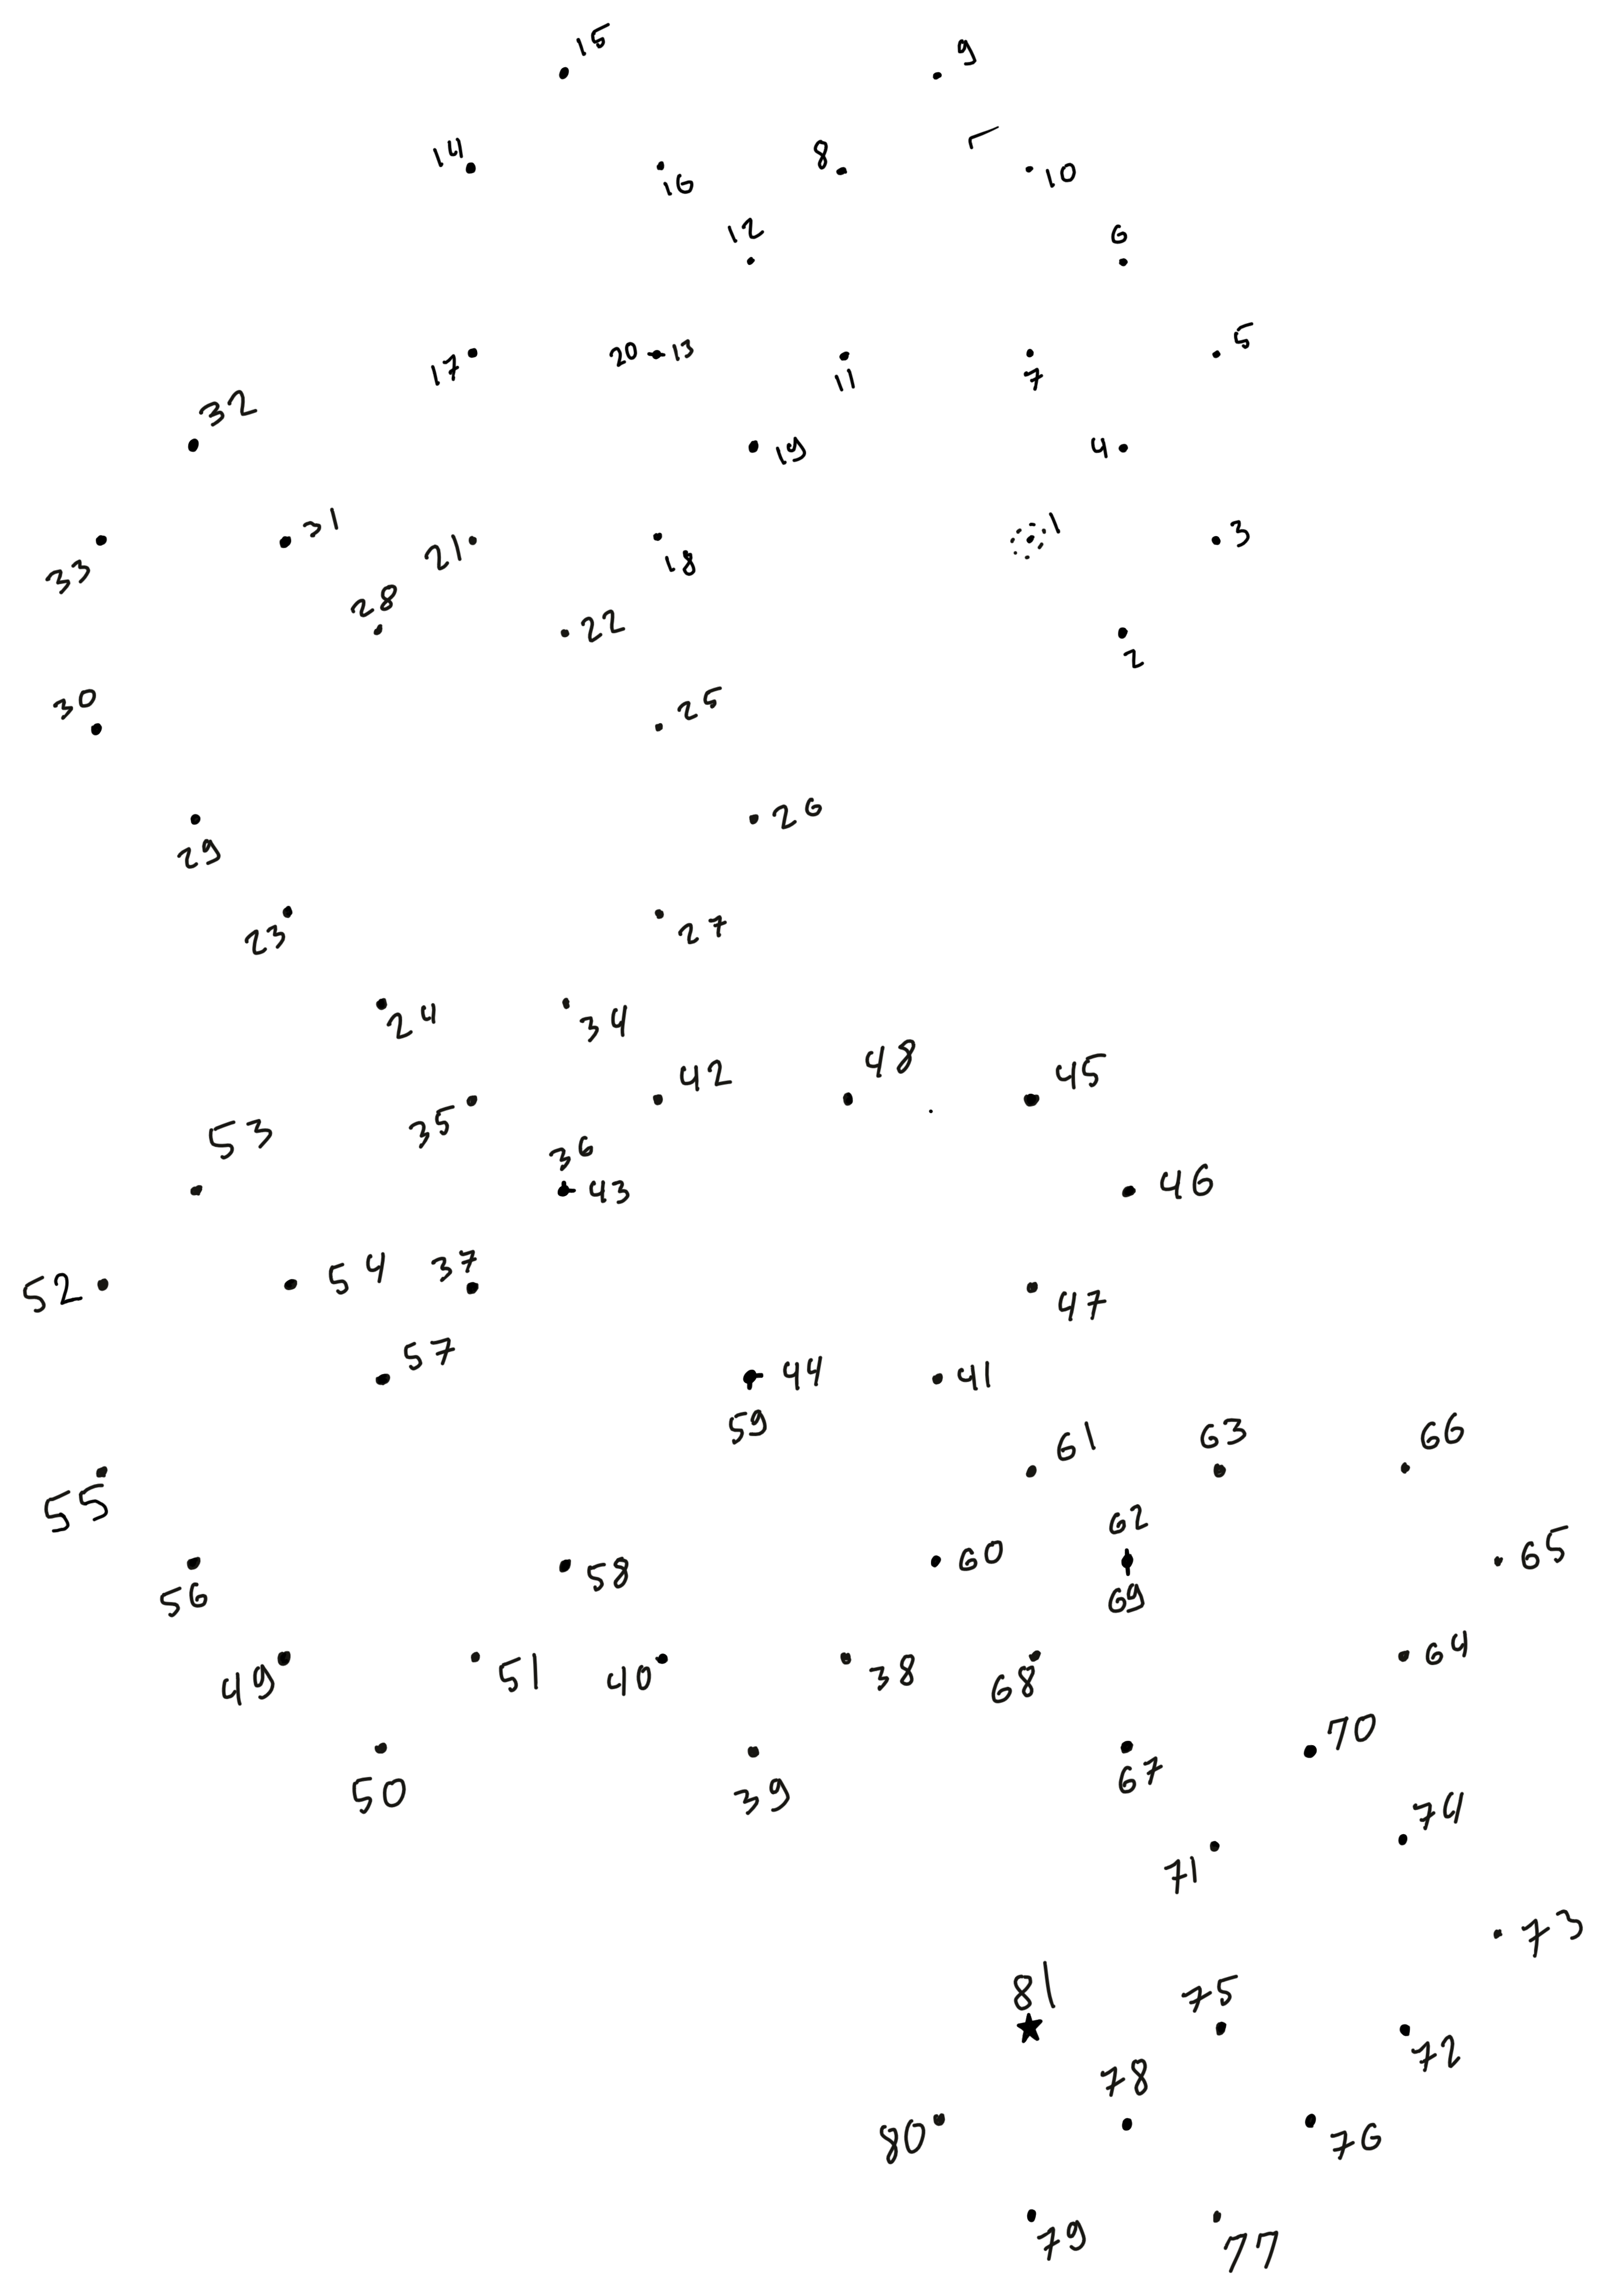
\includegraphics{A1AB5AFB-31BB-4E50-ABBE-7EDE8D4CA146.png}

This is a simple \emph{connect the dots} game. If you have this text
printed out and have a pencil handy, I encourage you to try it out and
discover the picture that hides behind those dots.

The point of this exercise is to show what happens to a linear variable
once it's consumed: It cannot be reused anymore. The dot pattern is
still visible, the numbers can still instruct you how to connect them.
But since the drawing has already been carried out, there is no possible
way to repeat the experience of connecting the dots.

Linear variables are the same, once they are used, they are ``spent''.
This is shown explicitly in Idris2's type system by using holes:

\begin{Shaded}
\begin{Highlighting}[]
\KeywordTok{let} \DecValTok{1}\NormalTok{ dots }\OtherTok{=} \DataTypeTok{MkDots}
    \DecValTok{1}\NormalTok{ drawing }\OtherTok{=}\NormalTok{ connect dots }\KeywordTok{in}
    \OperatorTok{?}\NormalTok{rest}
\end{Highlighting}
\end{Shaded}

inspecting the hole we get:

\begin{Shaded}
\begin{Highlighting}[]
\OperatorTok{\textgreater{}}  \DecValTok{0}\NormalTok{ dots }\OperatorTok{:} \DataTypeTok{Graph}
\OperatorTok{\textgreater{}}  \DecValTok{1}\NormalTok{ drawing }\OperatorTok{:} \DataTypeTok{Graph}
\OperatorTok{\textgreater{}} \CommentTok{{-}{-}{-}{-}{-}{-}{-}{-}{-}{-}{-}{-}{-}{-}{-}{-}{-}{-}{-}{-}{-}{-}{-}{-}{-}{-}{-}{-}{-}{-}}
\OperatorTok{\textgreater{}}\NormalTok{ rest }\OperatorTok{:} \DataTypeTok{Fun}
\end{Highlighting}
\end{Shaded}

Which indicates that, while we can still \emph{see} the dots, we cannot
do anything with them, they have linearity \texttt{0}. However, we ended
up with a \texttt{drawing} that we can now use! \footnote{You will
  notice that the program asks us to return a value of type \texttt{Fun}
  this is because the goal of this exercise is to have fun.}

\hypertarget{safe-inlining-with-1}{%
\paragraph{Safe inlining with 1}\label{safe-inlining-with-1}}

Linear variables have to be used exactly once, no less, no more. An
extremely nice property this gives us can be summarised with the
following statement:

\begin{quote}
A linear variable can always be safely inlined
\end{quote}

\emph{Inlining} refers to the ability of a compiler to replace a
function call by the implementation of the function. This is a typical
optimisation technique aimed at reducing the cost of function
calls\footnote{In low level programming, procedure calls require a
  context change where all the existing variables are stored in long
  term storage, then the procedure is called, then the result is stored
  somewhere, and finally the previous context is finally restored.} as
well as enabling further optimisations on the resulting program.

\emph{Safely inlined} means that the inlining process will not result in
a bigger and less efficient program. Take the following example:

\begin{Shaded}
\begin{Highlighting}[]
\KeywordTok{let}\NormalTok{ x }\OtherTok{=}\NormalTok{ f y }\KeywordTok{in}
\NormalTok{    (x, x)}
\end{Highlighting}
\end{Shaded}

After inlining \texttt{x}, that is, replace every occurrence of
\texttt{x} by its definition, we obtain:

\begin{Shaded}
\begin{Highlighting}[]
\NormalTok{(f y, f y)}
\end{Highlighting}
\end{Shaded}

Which is less efficient than the original program. Indeed, imagine that
\texttt{f} is a function that takes 5 days to run. The first case calls
\texttt{f} once and duplicates its result, which would take 5 days. But
the second case calls \texttt{f} twice, which would take 10 days in
total.

If \texttt{x} were to be \emph{linear} this problem would be caught:

\begin{Shaded}
\begin{Highlighting}[]
\KeywordTok{let} \DecValTok{1}\NormalTok{ x }\OtherTok{=}\NormalTok{ f y }\KeywordTok{in}
\NormalTok{    (x, x)}
\end{Highlighting}
\end{Shaded}

\begin{Shaded}
\begin{Highlighting}[]
\OperatorTok{\textgreater{}} \DataTypeTok{There}\NormalTok{ are }\DecValTok{2}\NormalTok{ uses }\KeywordTok{of}\NormalTok{ linear variable x}
\end{Highlighting}
\end{Shaded}

Conversely, if a program typechecks while using linear variable, then
all linear variables can be inlined without loss of performance. What's
more, inlining can provide further opportunities for optimisations down
the line. In the following example, while \texttt{y} cannot be inlined,
\texttt{x} can be.

\begin{Shaded}
\begin{Highlighting}[]
\KeywordTok{let} \DecValTok{1}\NormalTok{ x }\OtherTok{=} \DecValTok{1} \OperatorTok{+} \DecValTok{3} \KeywordTok{in}
\NormalTok{    y }\OtherTok{=}\NormalTok{ x }\OperatorTok{+} \DecValTok{10} \KeywordTok{in}
\NormalTok{    (y, y)}
\end{Highlighting}
\end{Shaded}

The result of inlining \texttt{x} would be as follows \footnote{This
  example does not quite work in Idris2 as it stands, we will talk about
  this topic in the ``QTT ergonomics'' section.}:

\begin{Shaded}
\begin{Highlighting}[]
\KeywordTok{let}\NormalTok{ y }\OtherTok{=} \DecValTok{1} \OperatorTok{+} \DecValTok{3} \OperatorTok{+} \DecValTok{10} \KeywordTok{in}
\NormalTok{    (y, y)}
\end{Highlighting}
\end{Shaded}

\hypertarget{erased-runtime-for-0}{%
\paragraph{Erased runtime for 0}\label{erased-runtime-for-0}}

In Idris2, variables can also be annotated with linearity \texttt{0},
this means that the value is \emph{inaccessible} and cannot be used. But
if that were truly the case, what would be the use of such a variable?

Those variables are particularly useful in a dependently-typed
programming language because, while they cannot be used in the body of
our program, they can be used in type signatures. Take this example with
vector:

\begin{Shaded}
\begin{Highlighting}[]
\FunctionTok{length} \OperatorTok{:} \DataTypeTok{Vect}\NormalTok{ n a }\OtherTok{{-}\textgreater{}} \DataTypeTok{Nat}
\FunctionTok{length}\NormalTok{ [] }\OtherTok{=} \DataTypeTok{Z}
\FunctionTok{length}\NormalTok{ (}\OtherTok{\_ ::}\NormalTok{ xs) }\OtherTok{=} \DataTypeTok{S}\NormalTok{ (}\FunctionTok{length}\NormalTok{ xs)}
\end{Highlighting}
\end{Shaded}

The length of the vector is computed by pattern matching on the vector
and recursively counting the length of the tail of the vector and adding
\texttt{+1} to it (recall the \texttt{S} constructor for \texttt{Nat}).
If the vector is empty, the length returned is zero (\texttt{Z}).

Another way to implement the same function in Idris1 (without linear
types) was to do the following:

\begin{Shaded}
\begin{Highlighting}[]
\CommentTok{{-}{-} This works in Idris1}
\FunctionTok{length} \OperatorTok{:} \DataTypeTok{Vect}\NormalTok{ n a }\OtherTok{{-}\textgreater{}} \DataTypeTok{Nat}
\FunctionTok{length}\NormalTok{ \_ \{n\} }\OtherTok{=}\NormalTok{ n}
\end{Highlighting}
\end{Shaded}

the \texttt{\{n\}} syntax would bring the value from the \emph{type
level} to the \emph{term level}, effectively making the type of the
vector a value that can be used within the program. However doing the
same in Idris2 is forbidden:

\begin{Shaded}
\begin{Highlighting}[]
\OperatorTok{\textgreater{}} \DataTypeTok{Error}\OperatorTok{:} \DataTypeTok{While}\NormalTok{ processing right hand side }\KeywordTok{of} \FunctionTok{length}\OperatorTok{.} 
\OperatorTok{\textgreater{}}\NormalTok{   n is }\FunctionTok{not}\NormalTok{ accessible }\KeywordTok{in}\NormalTok{ this context}\OperatorTok{.}
\OperatorTok{\textgreater{}} 
\OperatorTok{\textgreater{}}     \OperatorTok{|}
\OperatorTok{\textgreater{}}     \OperatorTok{|} \FunctionTok{length}\NormalTok{ \_ \{n\} }\OtherTok{=}\NormalTok{ n}
\OperatorTok{\textgreater{}}     \OperatorTok{|}                \OperatorTok{\^{}}
\end{Highlighting}
\end{Shaded}

It is hard to understand why this is the case just by looking at the
type signature \texttt{Vect\ n\ a\ -\textgreater{}\ Nat} and this is
because it is not complete. Behind the scenes, the Idris2 compiler is
adding implicit arguments \footnote{Implicit arguments are arguments to
  function that are not given by the programmer, but rather are filled
  in by the compiler automatically. Implicit arguments are extremely
  important in dependently-types languages because without them every
  type signature would be extremely heavy. Moreover, since the
  distinction between types and terms is blurry, the mechanism to infer
  \emph{types} is the same as the mechanism to infer \emph{terms} which
  is how the compiler can infer which value to insert whenever a
  function require an implicit argument.} for \texttt{n} and \texttt{a}
and automatically gives them linearity \texttt{0}. The full signature
looks like this:

\begin{Shaded}
\begin{Highlighting}[]
\FunctionTok{length} \OperatorTok{:}\NormalTok{ \{}\DecValTok{0}\NormalTok{ n }\OperatorTok{:} \DataTypeTok{Nat}\NormalTok{\} }\OtherTok{{-}\textgreater{}}\NormalTok{ \{}\DecValTok{0}\NormalTok{ a }\OperatorTok{:} \DataTypeTok{Type}\NormalTok{\} }\OtherTok{{-}\textgreater{}} \DataTypeTok{Vect}\NormalTok{ n a }\OtherTok{{-}\textgreater{}} \DataTypeTok{Nat}
\FunctionTok{length}\NormalTok{ \_ \{n\} }\OtherTok{=}\NormalTok{ n}
\end{Highlighting}
\end{Shaded}

The \texttt{0} means we cannot use the variable outside of type
signatures, but how come we can use them in the type signature and not
to implement our \texttt{length} function?

The difference is that linearity \texttt{0} variables are available
\emph{at compile time} and are forbidden to appear \emph{at runtime}.
The compiler can use them, compute types with them, but they cannot be
allocated and used during execution of the program we generate.

This is why linearity \texttt{0} variables are also called
\texttt{erased} variables because they are removed from the execution of
the program. We can use them to convince the compiler that some
invariants hold, but we cannot allocate any memory for them during the
execution of our program.

Finally, another subtlety is that erased variable can actually appear
inside the body of function, but only in position where they are
arguments to functions with \texttt{0} usage. Such functions are:

\hypertarget{arguments-annotated-with-0}{%
\subparagraph{\texorpdfstring{Arguments annotated with
\texttt{0}}{Arguments annotated with 0}}\label{arguments-annotated-with-0}}

\begin{Shaded}
\begin{Highlighting}[]
\NormalTok{toNat }\OperatorTok{:}\NormalTok{ (}\DecValTok{0}\NormalTok{ n }\OperatorTok{:} \DataTypeTok{Nat}\NormalTok{) }\OtherTok{{-}\textgreater{}} \DataTypeTok{INat}\NormalTok{ n }\OtherTok{{-}\textgreater{}} \DataTypeTok{Nat}
\NormalTok{toNat }\DataTypeTok{Z} \DataTypeTok{Zero} \OtherTok{=} \DataTypeTok{Z}
\NormalTok{toNat (}\DataTypeTok{S}\NormalTok{ n) (}\DataTypeTok{Succ}\NormalTok{ m) }\OtherTok{=} \DataTypeTok{S}\NormalTok{ (toNat n m)}
\CommentTok{{-}{-}       ▲                      ▲}
\CommentTok{{-}{-}       │                      └ Used even if erased}
\CommentTok{{-}{-}       │}
\CommentTok{{-}{-}       └ Bound with linearity 0}
\end{Highlighting}
\end{Shaded}

Here the recursive call uses \texttt{n} which has linearity \texttt{0},
but this is allowed because the first argument of \texttt{toNat} takes
an argument of linearity \texttt{0}. In other words, \texttt{n} cannot
be consumed, but \texttt{toNat} does not consume it's first argument
anyways, so all is good.

\hypertarget{rewrites}{%
\subparagraph{Rewrites}\label{rewrites}}

\begin{Shaded}
\begin{Highlighting}[]
\NormalTok{sym }\OperatorTok{:}\NormalTok{ (}\DecValTok{0}\NormalTok{ prf }\OperatorTok{:}\NormalTok{ x }\OtherTok{=}\NormalTok{ y) }\OtherTok{{-}\textgreater{}}\NormalTok{ y }\OtherTok{=}\NormalTok{ x}
\NormalTok{sym prf }\OtherTok{=}\NormalTok{ rewrite prf }\KeywordTok{in} \DataTypeTok{Refl}
\end{Highlighting}
\end{Shaded}

Rewriting a type does not consume the proof.

\hypertarget{type-signatures}{%
\subparagraph{Type signatures}\label{type-signatures}}

\begin{Shaded}
\begin{Highlighting}[]
\CommentTok{{-}{-}          ┌ \textasciigrave{}n\textasciigrave{} is erased}
\CommentTok{{-}{-}          ▼}
\NormalTok{reverse\textquotesingle{} }\OperatorTok{:}\NormalTok{ \{}\DecValTok{0}\NormalTok{ n }\OperatorTok{:} \DataTypeTok{Nat}\NormalTok{\} }\OtherTok{{-}\textgreater{}}\NormalTok{ (}\DecValTok{1}\NormalTok{ vs }\OperatorTok{:} \DataTypeTok{Vect}\NormalTok{ n }\DataTypeTok{Nat}\NormalTok{) }\OtherTok{{-}\textgreater{}} \DataTypeTok{Vect}\NormalTok{ n }\DataTypeTok{Nat}
\NormalTok{reverse\textquotesingle{} vs }\OtherTok{=} \KeywordTok{let}\NormalTok{ v2 }\OperatorTok{:} \DataTypeTok{Vect}\NormalTok{ n }\DataTypeTok{Nat} \OtherTok{=} \FunctionTok{reverse}\NormalTok{ vs }\KeywordTok{in}\NormalTok{ v2}
\CommentTok{{-}{-}                          ▲}
\CommentTok{{-}{-}                          └ \textasciigrave{}n\textasciigrave{} appears here}
\end{Highlighting}
\end{Shaded}

Even if \texttt{n} appears in the body of the function, appearing in a
type signature does not count as a use.

\hypertarget{no-branching-with-0}{%
\paragraph{No branching with 0}\label{no-branching-with-0}}

In general, we cannot match on erased variables, there is however an
exception to this rule. Whenever matching on a variable \emph{does not}
result in additional branching, then we are allowed to match on this
variable, even if it erased. Such matches are called
\emph{uninformative}, and they are characterised by the fact that they
do not generate new codepaths.

No new codepaths means that, whether we match or not, the output
bytecode would be the same. Except that matching on those variable would
inform us of very important properties from our types. Just like the
\texttt{intOrString} example informed us of the return type of our
function, an uninformative match can reveal useful information to both
the programmer and the compiler.

A good example of an uninformative match is \texttt{Refl} which has only
one constructor:

\begin{Shaded}
\begin{Highlighting}[]
\KeywordTok{data}\NormalTok{ (}\OtherTok{=}\NormalTok{) }\OperatorTok{:}\NormalTok{ (a, b }\OperatorTok{:} \DataTypeTok{Type}\NormalTok{) }\OtherTok{{-}\textgreater{}} \DataTypeTok{Type} \KeywordTok{where}
  \DataTypeTok{Refl} \OperatorTok{:}\NormalTok{ (a }\OperatorTok{:} \DataTypeTok{Type}\NormalTok{) }\OtherTok{{-}\textgreater{}}\NormalTok{ a }\OtherTok{=}\NormalTok{ a}
\end{Highlighting}
\end{Shaded}

This suggests that, even if our equality proof has linearity \texttt{0},
we can match on it, since there is only 1 constructor we are never going
to generate new branches.

But an uninformative match can also happen on types with multiple
constructors. Take this indexed \footnote{A \emph{type parameter} that
  changes with the values that inhabit the type. For example
  \texttt{{[}"a",\ "b",\ "c"{]}\ :\ Vect\ 3\ String} has index
  \texttt{3} and a type parameter \texttt{String}, because it has 3
  elements and the elements are Strings.} \texttt{Nat} type:

\begin{Shaded}
\begin{Highlighting}[]
\KeywordTok{data} \DataTypeTok{INat} \OperatorTok{:} \DataTypeTok{Nat} \OtherTok{{-}\textgreater{}} \DataTypeTok{Type} \KeywordTok{where}
  \DataTypeTok{IZ} \OperatorTok{:} \DataTypeTok{INat} \DataTypeTok{Z}
  \DataTypeTok{IS} \OperatorTok{:} \DataTypeTok{INat}\NormalTok{ n }\OtherTok{{-}\textgreater{}} \DataTypeTok{INat}\NormalTok{ (}\DataTypeTok{S}\NormalTok{ n)}
\end{Highlighting}
\end{Shaded}

This is simply a duplicate for \texttt{Nat} but carries its own value as
index. Now let us write a function to recover the original \texttt{Nat}
from an \texttt{INat}:

\begin{Shaded}
\begin{Highlighting}[]
\NormalTok{toNat }\OperatorTok{:}\NormalTok{ (}\DecValTok{0}\NormalTok{ n }\OperatorTok{:} \DataTypeTok{Nat}\NormalTok{) }\OtherTok{{-}\textgreater{}}\NormalTok{ (}\DecValTok{1}\NormalTok{ m }\OperatorTok{:} \DataTypeTok{INat}\NormalTok{ n) }\OtherTok{{-}\textgreater{}} \DataTypeTok{Nat}
\NormalTok{toNat }\DataTypeTok{Z} \DataTypeTok{IZ} \OtherTok{=} \DataTypeTok{Z}
\NormalTok{toNat (}\DataTypeTok{S}\NormalTok{ n) (}\DataTypeTok{IS}\NormalTok{ m) }\OtherTok{=} \DataTypeTok{S}\NormalTok{ (toNat n m)}
\end{Highlighting}
\end{Shaded}

Even if we annotated \texttt{n} with linearity \texttt{0} we are allowed
to match on it. To understand why, let us add some holes and remove the
matching:

\begin{Shaded}
\begin{Highlighting}[]
\NormalTok{toNat }\OperatorTok{:}\NormalTok{ (}\DecValTok{0}\NormalTok{ n }\OperatorTok{:} \DataTypeTok{Nat}\NormalTok{) }\OtherTok{{-}\textgreater{}}\NormalTok{ (}\DecValTok{1}\NormalTok{ m }\OperatorTok{:} \DataTypeTok{INat}\NormalTok{ n) }\OtherTok{{-}\textgreater{}} \DataTypeTok{Nat}
\NormalTok{toNat n }\DataTypeTok{IZ} \OtherTok{=} \OperatorTok{?}\NormalTok{branch}
\NormalTok{toNat (}\DataTypeTok{S}\NormalTok{ n) (}\DataTypeTok{IS}\NormalTok{ m) }\OtherTok{=} \DataTypeTok{S}\NormalTok{ (toNat n m)}
\end{Highlighting}
\end{Shaded}

Idris2 will not allow this program to compile and will fail with the
following error:

\begin{Shaded}
\begin{Highlighting}[]
\OperatorTok{\textgreater{}} \DataTypeTok{Error}\OperatorTok{:} \DataTypeTok{While}\NormalTok{ processing left hand side }\KeywordTok{of}\NormalTok{ toNat}\OperatorTok{.} 
\OperatorTok{\textgreater{}}   \DataTypeTok{When}\NormalTok{ unifying }\DataTypeTok{INat} \DecValTok{0} \FunctionTok{and} \DataTypeTok{INat} \OperatorTok{?}\NormalTok{n}\OperatorTok{.}
\OperatorTok{\textgreater{}} \DataTypeTok{Pattern}\NormalTok{ variable n unifies with}\OperatorTok{:} \DecValTok{0}\OperatorTok{.}
\OperatorTok{\textgreater{}} 
\OperatorTok{\textgreater{}}     \OperatorTok{|}
\OperatorTok{\textgreater{}}     \OperatorTok{|}   \DataTypeTok{IZ} \OperatorTok{:} \DataTypeTok{INat} \DataTypeTok{Z}
\OperatorTok{\textgreater{}}     \OperatorTok{|}             \OperatorTok{\^{}}
\OperatorTok{\textgreater{}}     \OperatorTok{|}   \DataTypeTok{IS} \OperatorTok{:} \DataTypeTok{INat}\NormalTok{ n }\OtherTok{{-}\textgreater{}} \DataTypeTok{INat}\NormalTok{ (}\DataTypeTok{S}\NormalTok{ n)}
\OperatorTok{\textgreater{}}     \OperatorTok{|}\NormalTok{  toNat n }\DataTypeTok{IZ} \OtherTok{=} \OperatorTok{?}\NormalTok{branch}
\OperatorTok{\textgreater{}}     \OperatorTok{|}        \OperatorTok{\^{}}
\OperatorTok{\textgreater{}} 
\OperatorTok{\textgreater{}} \DataTypeTok{Suggestion}\OperatorTok{:} \DataTypeTok{Use}\NormalTok{ the same name for both }\KeywordTok{pattern}\NormalTok{ variables, since they }
\OperatorTok{\textgreater{}}\NormalTok{   unify}\OperatorTok{.}
\end{Highlighting}
\end{Shaded}

It tells us that \texttt{n} unifies with \texttt{Z} and forces the user
to spell out the match. Effectively forcing uninformative matches to be
made. A similar error appears if we try the same thing on the second
branch, trying to remove \texttt{S\ n}.

\hypertarget{the-story-begins}{%
\subsection{The story begins}\label{the-story-begins}}

This concludes our introductory chapter. I suggest you come back to it
regularly to brush up on the linear concepts, pay particular attention
to the ``linear intuition'' section in order to make sense of
\emph{erased} variables and \emph{linear} variables. I also want to
stress that at the end is a glossary that lists all the important terms
and concepts necessary to understand the body of this work. Please feel
free to consult it if something is unclear.

In the next section I will start listing and describing uses of linear
types, and what happens when they are combined with dependent types.
Some of them were already known, but some of them are also new and
delightful.

\hypertarget{quantitative-type-theory-in-practice}{%
\section{Quantitative Type Theory in
practice}\label{quantitative-type-theory-in-practice}}

Linear types haven't really found a place in mainstream commercial
application of software engineering. Becase qtt is even more niche than
linear logic and because it's much newer it hasn't seen almost
\emph{any} use under any shape or form. The Idris2 compiler itself
stands as the most popular example of a complex program that showcases
uses for QTT and quantitative types. For this reason, while this section
does not provide any concrete contributions, I thought it was warranted
to list some new, innovative and unexpected uses for linear types and
QTT.

\hypertarget{opening-the-door-to-new-opportunities}{%
\subsection{Opening the door to new
opportunities}\label{opening-the-door-to-new-opportunities}}

The door protocol lol

\hypertarget{limitations-and-solutions-for-quantitative-types}{%
\subsection{limitations and solutions for quantitative
types}\label{limitations-and-solutions-for-quantitative-types}}

We've seen how we can write addition of natural numbers using linear
types. But can we write a multiplication algorithm using linear types?
Let us inspect the traditional multiplication algorithm and see if we
can update it with linear types.

\hypertarget{linear-multiplication}{%
\subsubsection{Linear multiplication}\label{linear-multiplication}}

Here is a multiplication function without any linear variables

\begin{Shaded}
\begin{Highlighting}[]
\NormalTok{multiplication }\OperatorTok{:}\NormalTok{ (n }\OperatorTok{:} \DataTypeTok{Nat}\NormalTok{) }\OtherTok{{-}\textgreater{}}\NormalTok{ (m }\OperatorTok{:} \DataTypeTok{Nat}\NormalTok{) }\OtherTok{{-}\textgreater{}} \DataTypeTok{Nat}
\NormalTok{multiplication }\DataTypeTok{Z}\NormalTok{ m }\OtherTok{=} \DataTypeTok{Z} 
\NormalTok{multiplication (}\DataTypeTok{S}\NormalTok{ n) m }\OtherTok{=}\NormalTok{ m }\OperatorTok{+}\NormalTok{ (multiplication n m)}
\end{Highlighting}
\end{Shaded}

Just like with addition, we notice that some variables are only used
once, but some aren't. \texttt{n} is used exactly once in both branches,
but \texttt{m} is not used in one branch, and used twice in the other.
Which leads to the following program:

\begin{Shaded}
\begin{Highlighting}[]
\NormalTok{ multiplication }\OperatorTok{:}\NormalTok{ (}\DecValTok{1}\NormalTok{ n }\OperatorTok{:} \DataTypeTok{Nat}\NormalTok{) }\OtherTok{{-}\textgreater{}}\NormalTok{ (m }\OperatorTok{:} \DataTypeTok{Nat}\NormalTok{) }\OtherTok{{-}\textgreater{}} \DataTypeTok{Nat}
\NormalTok{ multiplication }\DataTypeTok{Z}\NormalTok{ m }\OtherTok{=} \DataTypeTok{Z}
\NormalTok{ multiplication (}\DataTypeTok{S}\NormalTok{ n) m }\OtherTok{=}\NormalTok{ m }\OperatorTok{+}\NormalTok{ (multiplication n m)}
\end{Highlighting}
\end{Shaded}

Which compiles correctly, but how could we go about implementing a
completely linear version of \texttt{mutliplication}?

indeed, writing
\texttt{multiplication\ :\ (1\ n\ :\ Nat)\ -\textgreater{}\ (0\ m\ :\ Nat)\ -\textgreater{}\ Nat}
gets us the error:

\begin{Shaded}
\begin{Highlighting}[]
\DataTypeTok{Error}\OperatorTok{:} \DataTypeTok{While}\NormalTok{ processing right hand side }\KeywordTok{of}\NormalTok{ multiplication}\OperatorTok{.}\NormalTok{ m is }\FunctionTok{not}\NormalTok{ accessible }\KeywordTok{in}\NormalTok{ this context}\OperatorTok{.}

    \OperatorTok{|}
    \OperatorTok{|}\NormalTok{ multiplication (}\DataTypeTok{S}\NormalTok{ n) m }\OtherTok{=}\NormalTok{ m }\OperatorTok{+}\NormalTok{ (multiplication n m)}
    \OperatorTok{|}                          \OperatorTok{\^{}}
\end{Highlighting}
\end{Shaded}

Which catches the fact that \texttt{m} is use twice in the second branch
(but the first branch is fine).

Ideally we would like to write this program:

\begin{Shaded}
\begin{Highlighting}[]
\CommentTok{{-}{-}        The multiplicity depends on the first arugment}
\CommentTok{{-}{-}                               v}
\NormalTok{multiplication }\OperatorTok{:}\NormalTok{ (}\DecValTok{1}\NormalTok{ n }\OperatorTok{:} \DataTypeTok{Nat}\NormalTok{) }\OtherTok{{-}\textgreater{}}\NormalTok{ (n m }\OperatorTok{:} \DataTypeTok{Nat}\NormalTok{) }\OtherTok{{-}\textgreater{}} \DataTypeTok{Nat}
\NormalTok{multiplication }\DataTypeTok{Z}\NormalTok{ m }\OtherTok{=} \DataTypeTok{Z}
\NormalTok{multiplication (}\DataTypeTok{S}\NormalTok{ n) m }\OtherTok{=}\NormalTok{ m }\OperatorTok{+}\NormalTok{ (multiplication n m)}
\end{Highlighting}
\end{Shaded}

However Idris2 and QTT do not support \emph{dependent linearities} or
\emph{first class linearity} where linearity annotations are values
within the language.

We can however attempt to replicate this behaviour with different
proxies:

\begin{Shaded}
\begin{Highlighting}[]
\NormalTok{provide }\OperatorTok{:} \DataTypeTok{Copy}\NormalTok{ t }\OtherTok{=\textgreater{}} \DataTypeTok{Drop}\NormalTok{ t }\OtherTok{=\textgreater{}}\NormalTok{ (}\DecValTok{1}\NormalTok{ n }\OperatorTok{:} \DataTypeTok{Nat}\NormalTok{) }\OtherTok{{-}\textgreater{}}\NormalTok{ (}\DecValTok{1}\NormalTok{ v }\OperatorTok{:}\NormalTok{ t) }\OtherTok{{-}\textgreater{}}\NormalTok{ (}\DataTypeTok{DPair} \DataTypeTok{Nat}\NormalTok{ (\textbackslash{}x }\OtherTok{=\textgreater{}}\NormalTok{ n }\OtherTok{=}\NormalTok{ x), }\DataTypeTok{Vect}\NormalTok{ n t)}
\NormalTok{provide }\DecValTok{0}\NormalTok{ v }\OtherTok{=} \KeywordTok{let}\NormalTok{ () }\OtherTok{=} \FunctionTok{drop}\NormalTok{ v }\KeywordTok{in}\NormalTok{ (}\DataTypeTok{MkDPair} \DataTypeTok{Z} \DataTypeTok{Refl}\NormalTok{, [])}
\NormalTok{provide (}\DataTypeTok{S}\NormalTok{ k) v }\OtherTok{=} \KeywordTok{let}\NormalTok{ (v1, v2) }\OtherTok{=}\NormalTok{ copy v}
\NormalTok{                      (}\DataTypeTok{MkDPair}\NormalTok{ n prf, vs) }\OtherTok{=}\NormalTok{ provide k v1 }\KeywordTok{in} \DataTypeTok{MkDPair}\NormalTok{ (}\DataTypeTok{S}\NormalTok{ n) (cong }\DataTypeTok{S}\NormalTok{ prf),}\OtherTok{ v2 ::}\NormalTok{ vs)}

\NormalTok{multiplication }\OperatorTok{:}\NormalTok{ (}\DecValTok{1}\NormalTok{ n, m }\OperatorTok{:} \DataTypeTok{Nat}\NormalTok{) }\OtherTok{{-}\textgreater{}} \DataTypeTok{Nat}
\NormalTok{multiplication n m }\OtherTok{=} \KeywordTok{let}\NormalTok{ (}\DataTypeTok{MkDPair}\NormalTok{ n\textquotesingle{} }\DataTypeTok{Refl}\NormalTok{, ms) }\OtherTok{=}\NormalTok{ provide n m }\KeywordTok{in}\NormalTok{ mult n\textquotesingle{} ms}
  \KeywordTok{where}
\NormalTok{    mult }\OperatorTok{:}\NormalTok{ (}\DecValTok{1}\NormalTok{ n }\OperatorTok{:} \DataTypeTok{Nat}\NormalTok{) }\OtherTok{{-}\textgreater{}}\NormalTok{ (}\DecValTok{1}\NormalTok{ vs }\OperatorTok{:} \DataTypeTok{Vect}\NormalTok{ n }\DataTypeTok{Nat}\NormalTok{) }\OtherTok{{-}\textgreater{}} \DataTypeTok{Nat}
\NormalTok{    mult }\DecValTok{0}\NormalTok{ [] }\OtherTok{=} \DecValTok{0}
\NormalTok{    mult (}\DataTypeTok{S}\NormalTok{ k) (}\OtherTok{m ::}\NormalTok{ x) }\OtherTok{=}\NormalTok{ m }\OperatorTok{+}\NormalTok{ (mult k x)}
\end{Highlighting}
\end{Shaded}

This program attempts to simulate the previous signature by creating a
dependency between \texttt{n} and a vector of length \texttt{n}
containing copies of the variable \texttt{m}\footnote{For the purposes
  of this example there is no proof that the vector \emph{actually}
  contains only copies of \texttt{m} but this is an invariant that could
  be implemented at the type level with a data structure like the
  following:

  \texttt{data\ NCopies\ :\ (n\ :\ Nat)\ -\textbackslash{}\textgreater{}\ (t\ :\ Type)\ -\textbackslash{}\textgreater{}\ (v\ :\ t)-\textbackslash{}\textgreater{}\ Type\ where}
  Empty : NCopies Z t v `` More : (1 v : t) -\textgreater{} (1 vs :
  NCopies n t v) -\textgreater{} NCopies (S n) t v

  The example given uses \texttt{Vect} for brevity and readability, the
  code quickly becomes unwieldy with equality proofs everywhere, which
  aren't the point of the example, nor showcase linear types.} with the
type
\texttt{mult\ :\ (1\ n\ :\ Nat)\ -\textgreater{}\ (1\ \_\ :\ Vect\ n\ Nat)\ -\textgreater{}\ Nat~}.

As we've demonstrated, we technically can express more complex
relationship between linear types provided they implement our interfaces
\texttt{Drop} and \texttt{Copy}. However, the extra work to make the
dependency explicit in the type isn't worth the effort. Indeed, giving
up this dependency allows us to write the following program:

\begin{Shaded}
\begin{Highlighting}[]
\NormalTok{lmult }\OperatorTok{:}\NormalTok{ (}\DecValTok{1}\NormalTok{ n, m }\OperatorTok{:} \DataTypeTok{Nat}\NormalTok{) }\OtherTok{{-}\textgreater{}} \DataTypeTok{Nat}
\NormalTok{lmult }\DecValTok{0}\NormalTok{ m }\OtherTok{=} \KeywordTok{let}\NormalTok{ () }\OtherTok{=} \FunctionTok{drop}\NormalTok{ m }\KeywordTok{in} \DataTypeTok{Z}
\NormalTok{lmult (}\DataTypeTok{S}\NormalTok{ k) m }\OtherTok{=} \KeywordTok{let}\NormalTok{ (a, b) }\OtherTok{=}\NormalTok{ copy m }\KeywordTok{in}\NormalTok{ a }\OperatorTok{+}\NormalTok{ lmult k b}
\end{Highlighting}
\end{Shaded}

Which is a lot simpler and achieves the same goal, it even has the same
performance characteristics.

\hypertarget{more-granular-dependencies}{%
\subsubsection{More granular
dependencies}\label{more-granular-dependencies}}

While our previous example has only be mildly successful, there exist a
language that can express our idea, and that is \emph{Granule}.

Granule is a programming language with \emph{graded modal types}, types
which rely on \emph{graded modalities}. Those are annotation that span a
\emph{range} of different values in order to describe each type. Those
values can themselves be paired up together and combined in order to
represent even more complex behaviour than our linear multiplication.
For now, let us stick to multiplication and see what a future version of
Idris supporting graded modalities could look like.

Granule's syntax is very close to Idris, Agda and Haskell, however,
linearity in \emph{Granule} is the default so there is nothing to
specify for a linear variable. In addition, \texttt{Nat} is not a
\texttt{Type} in \emph{Granule} but a \emph{modality}, which means, in
order to work with \texttt{Nat} and write dependencies between them we
will create a data type indexed on \texttt{Nat}:

\begin{Shaded}
\begin{Highlighting}[]
\KeywordTok{data} \DataTypeTok{INat}\NormalTok{ (n }\OperatorTok{:} \DataTypeTok{Nat}\NormalTok{) }\KeywordTok{where}
  \DataTypeTok{Z} \OperatorTok{:} \DataTypeTok{INat} \DecValTok{0}\NormalTok{;}
  \DataTypeTok{S} \OperatorTok{:} \DataTypeTok{INat}\NormalTok{ n }\OtherTok{{-}\textgreater{}} \DataTypeTok{INat}\NormalTok{ (n }\OperatorTok{+} \DecValTok{1}\NormalTok{)}
\end{Highlighting}
\end{Shaded}

This allows us to write the add function as follows:

\begin{Shaded}
\begin{Highlighting}[]
\NormalTok{linearAdd }\OperatorTok{:} \KeywordTok{forall}\NormalTok{ \{n m }\OperatorTok{:} \DataTypeTok{Nat}\NormalTok{\} }\OperatorTok{.} \DataTypeTok{INat}\NormalTok{ n }\OtherTok{{-}\textgreater{}} \DataTypeTok{INat}\NormalTok{ m }\OtherTok{{-}\textgreater{}} \DataTypeTok{INat}\NormalTok{ (n }\OperatorTok{+}\NormalTok{ m)}
\NormalTok{linearAdd }\DataTypeTok{Z}\NormalTok{ m }\OtherTok{=}\NormalTok{ m;}
\NormalTok{linearAdd (}\DataTypeTok{S}\NormalTok{ n) m }\OtherTok{=} \DataTypeTok{S}\NormalTok{ (linearAdd n m)}
\end{Highlighting}
\end{Shaded}

If we were to omit the \texttt{m} in the first branch and write
\texttt{linearAdd\ Z\ m\ =\ Z} we would get the error:

\begin{Shaded}
\begin{Highlighting}[]
\DataTypeTok{Linearity} \FunctionTok{error}\OperatorTok{:}\NormalTok{ multiplication}\OperatorTok{.}\NormalTok{gr}\OperatorTok{:}
\DataTypeTok{Linear}\NormalTok{ variable }\OtherTok{\textasciigrave{}m\textasciigrave{}}\NormalTok{ is never used}\OperatorTok{.}
\end{Highlighting}
\end{Shaded}

Which is what we expect.

Now that we have indexed \texttt{Nat} we can try again our
\texttt{multiplication} function:

\begin{Shaded}
\begin{Highlighting}[]
\NormalTok{multiplication }\OperatorTok{:} \KeywordTok{forall}\NormalTok{ \{n m }\OperatorTok{:} \DataTypeTok{Nat}\NormalTok{\} }\OperatorTok{.} \DataTypeTok{INat}\NormalTok{ n }\OtherTok{{-}\textgreater{}}\NormalTok{ (}\DataTypeTok{INat}\NormalTok{ m) [n] }\OtherTok{{-}\textgreater{}} \DataTypeTok{INat}\NormalTok{ (n }\OperatorTok{*}\NormalTok{ m)}
\NormalTok{multiplication }\DataTypeTok{Z}\NormalTok{ [m] }\OtherTok{=} \DataTypeTok{Z}\NormalTok{;}
\NormalTok{multiplication (}\DataTypeTok{S}\NormalTok{ n) [m] }\OtherTok{=}\NormalTok{ linearAdd m (multiplication n m)}
\end{Highlighting}
\end{Shaded}

As you can see, we annotate the second argument of the type signature
with \texttt{{[}n{]}} which indicates that the modality of the second
argument depends on the value of the first argument. This syntax repeats
in the implementation where the second argument \texttt{m} has to be
``unboxed'' using the \texttt{{[}m{]}} syntax which will tell the
compiler to correctly infer the usage allowed by the indexed modality.
In the first branch there are \texttt{0} uses available, and in the
second there are \texttt{n\ +\ 1} uses available.

While \emph{Granule} doesn't have dependent types, indexed types are
enough to show interesting programs such as multiplication. More recent
developments have made progress toward implementing full type dependency
between quantities and terms in the language.

\hypertarget{permutations}{%
\subsection{Permutations}\label{permutations}}

During my time on this Master program I was also working for a
commercial company using Idris for their business: Statebox.

One of their project is a validator for petri-nets and petri-net
executions: \href{https://github.com/statebox/fsm-oracle}{FSM-oracle}.
While the technical details of this projects are outside the scope of
this text, there is one aspect of it that is fundamentally linked with
linear types, and that is the concept of permutation.

FSM-Oracle describes petri-nets using
\href{http://www.zanasi.com/fabio/files/paperCALCO19b.pdf}{\emph{hypergraphs}}
those hypergraphs have a concept of
\href{https://github.com/statebox/fsm-oracle/blob/master/src/Permutations/Permutations.idr\#L31}{\emph{permutation}~}
that allows to move wires around. This concept is key in a correct and
proven implementation of hypergraphs. However, permutations also turn
out to be extremely complex to implement as can attest the files
\href{https://github.com/statebox/fsm-oracle/blob/master/src/Permutations/PermutationsCategory.idr}{trying
to fit} their definition into a
\href{https://github.com/statebox/fsm-oracle/blob/master/src/Permutations/PermutationsStrictMonoidalCategory.idr}{Category}.

Linear types can thankfully ease the pain by providing a very simple
representation of permutations:

\begin{Shaded}
\begin{Highlighting}[]
\DataTypeTok{Permutation} \OperatorTok{:} \DataTypeTok{Type} \OtherTok{{-}\textgreater{}} \DataTypeTok{Type}
\DataTypeTok{Premutation}\NormalTok{ a }\OtherTok{=}\NormalTok{ (}\DecValTok{1}\NormalTok{ ls }\OperatorTok{:} \DataTypeTok{List}\NormalTok{ a) }\OtherTok{{-}\textgreater{}} \DataTypeTok{List}\NormalTok{ a}
\end{Highlighting}
\end{Shaded}

That is, a \texttt{Permutation} parameterised over a type \texttt{a} is
a linear function from \texttt{List\ a} to \texttt{List\ a}.

This definition works because no elements from the input list can be
omited or reused for the output list. \emph{Every single element} from
the argument has to find a new spot in the output list. Additionally,
since the type \texttt{a} is unknown, no special value can be inserted
in advance. Indeed, the only way to achieve this effect would be to
pattern match on \texttt{a} and create values once \texttt{a} is known,
but this would require \texttt{a} to be bound with a multiplicity
greater than \texttt{0}:

\begin{Shaded}
\begin{Highlighting}[]
\NormalTok{fakePermutation }\OperatorTok{:}\NormalTok{ \{a }\OperatorTok{:} \DataTypeTok{Type}\NormalTok{\} }\OtherTok{{-}\textgreater{}}\NormalTok{ (}\DecValTok{1}\NormalTok{ \_ }\OperatorTok{:} \DataTypeTok{List}\NormalTok{ a) }\OtherTok{{-}\textgreater{}} \DataTypeTok{List}\NormalTok{ a}
\NormalTok{fakePermutatoin \{a }\OtherTok{=} \DataTypeTok{Int}\NormalTok{\} ls }\OtherTok{=} \DecValTok{42}\OtherTok{ ::}\NormalTok{ ls}
\NormalTok{fakePermutation \{a }\OtherTok{=}\NormalTok{ \_\} ls }\OtherTok{=} \FunctionTok{reverse}\NormalTok{ ls}
\end{Highlighting}
\end{Shaded}

In this example, \texttt{a} is bound with \emph{unrestricted}
multiplicity, which give us the hint that it \emph{is} inspected and the
permutation might not be a legitimate permutation.

What's more, viewing permutations as a function gives it extremely
simple categorical semantics: It is just an instance of the category of
types with linear functions as morphisms.

Assuming \texttt{Category} is defined this way:

\begin{Shaded}
\begin{Highlighting}[]
\CommentTok{{-}{-} operator for composition}
\NormalTok{infix }\DecValTok{2} \OperatorTok{.*.}
\CommentTok{{-}{-} operator for morphisms}
\KeywordTok{infixr} \DecValTok{1} \OperatorTok{\textasciitilde{}\textgreater{}}

\NormalTok{record }\DataTypeTok{Category}\NormalTok{ (obj }\OperatorTok{:} \DataTypeTok{Type}\NormalTok{)  }\KeywordTok{where}
\NormalTok{  constructor }\DataTypeTok{MkCategory}
\NormalTok{  (}\OperatorTok{\textasciitilde{}\textgreater{}}\NormalTok{)          }\OperatorTok{:}\NormalTok{ obj }\OtherTok{{-}\textgreater{}}\NormalTok{ obj }\OtherTok{{-}\textgreater{}} \DataTypeTok{Type} \CommentTok{{-}{-} morphism}
\NormalTok{  identity      }\OperatorTok{:}\NormalTok{ \{}\DecValTok{0}\NormalTok{ a }\OperatorTok{:}\NormalTok{ obj\} }\OtherTok{{-}\textgreater{}}\NormalTok{ a }\OperatorTok{\textasciitilde{}\textgreater{}}\NormalTok{ a}
\NormalTok{  (}\OperatorTok{.*.}\NormalTok{)         }\OperatorTok{:}\NormalTok{ \{}\DecValTok{0}\NormalTok{ a, b, c}\OperatorTok{:}\NormalTok{ obj\}}
               \OtherTok{{-}\textgreater{}}\NormalTok{ (a }\OperatorTok{\textasciitilde{}\textgreater{}}\NormalTok{ b)}
               \OtherTok{{-}\textgreater{}}\NormalTok{ (b }\OperatorTok{\textasciitilde{}\textgreater{}}\NormalTok{ c)}
               \OtherTok{{-}\textgreater{}}\NormalTok{ (a }\OperatorTok{\textasciitilde{}\textgreater{}}\NormalTok{ c)}
\NormalTok{  leftIdentity  }\OperatorTok{:}\NormalTok{ \{}\DecValTok{0}\NormalTok{ a, b }\OperatorTok{:}\NormalTok{ obj\}}
               \OtherTok{{-}\textgreater{}}\NormalTok{ (f }\OperatorTok{:}\NormalTok{ a }\OperatorTok{\textasciitilde{}\textgreater{}}\NormalTok{ b)}
               \OtherTok{{-}\textgreater{}}\NormalTok{ identity }\OperatorTok{.*.}\NormalTok{ f }\OtherTok{=}\NormalTok{ f}
\NormalTok{  rightIdentity }\OperatorTok{:}\NormalTok{ \{}\DecValTok{0}\NormalTok{ a, b }\OperatorTok{:}\NormalTok{ obj\}}
               \OtherTok{{-}\textgreater{}}\NormalTok{ (f }\OperatorTok{:}\NormalTok{ a }\OperatorTok{\textasciitilde{}\textgreater{}}\NormalTok{ b)}
               \OtherTok{{-}\textgreater{}}\NormalTok{ f }\OperatorTok{.*.}\NormalTok{ identity }\OtherTok{=}\NormalTok{ f}
\NormalTok{  associativity }\OperatorTok{:}\NormalTok{ \{}\DecValTok{0}\NormalTok{ a, b, c, d }\OperatorTok{:}\NormalTok{ obj\}}
               \OtherTok{{-}\textgreater{}}\NormalTok{ (f }\OperatorTok{:}\NormalTok{ a }\OperatorTok{\textasciitilde{}\textgreater{}}\NormalTok{ b)}
               \OtherTok{{-}\textgreater{}}\NormalTok{ (g }\OperatorTok{:}\NormalTok{ b }\OperatorTok{\textasciitilde{}\textgreater{}}\NormalTok{ c)}
               \OtherTok{{-}\textgreater{}}\NormalTok{ (h }\OperatorTok{:}\NormalTok{ c }\OperatorTok{\textasciitilde{}\textgreater{}}\NormalTok{ d)}
               \OtherTok{{-}\textgreater{}}\NormalTok{ f }\OperatorTok{.*.}\NormalTok{ (g }\OperatorTok{.*.}\NormalTok{ h) }\OtherTok{=}\NormalTok{ (f }\OperatorTok{.*.}\NormalTok{ g) }\OperatorTok{.*.}\NormalTok{ h}
\end{Highlighting}
\end{Shaded}

We can write and instance of \texttt{Category} for \texttt{List\ o}:

\begin{Shaded}
\begin{Highlighting}[]
\DataTypeTok{Permutation} \OperatorTok{:} \DataTypeTok{List}\NormalTok{ o }\OtherTok{{-}\textgreater{}} \DataTypeTok{List}\NormalTok{ o }\OtherTok{{-}\textgreater{}} \DataTypeTok{Type}
\DataTypeTok{Permutation}\NormalTok{ a b }\OtherTok{=} \DataTypeTok{Same}\NormalTok{ a b}

\NormalTok{permutationCategory }\OperatorTok{:} \DataTypeTok{Category}\NormalTok{ (}\DataTypeTok{List}\NormalTok{ o)}
\NormalTok{permutationCategory }\OtherTok{=} \DataTypeTok{MkCategory}
  \DataTypeTok{Permutation}
\NormalTok{  sid}
\NormalTok{  linCompose}
\NormalTok{  linLeftIdentity}
\NormalTok{  linRightIdentity}
\NormalTok{  linAssoc}
\end{Highlighting}
\end{Shaded}

Using the definitions and lemmas for \texttt{Same} which is a data type
that represents a linear function between two values of the same type:

\begin{Shaded}
\begin{Highlighting}[]
\CommentTok{{-}{-} a linear function between two values of the same type}
\NormalTok{record }\DataTypeTok{Same}\NormalTok{ \{}\DecValTok{0}\NormalTok{ o }\OperatorTok{:} \DataTypeTok{Type}\NormalTok{\} (input, output }\OperatorTok{:}\NormalTok{ o) }\KeywordTok{where}
\NormalTok{  constructor }\DataTypeTok{MkSame}
\NormalTok{  func }\OperatorTok{:} \DataTypeTok{LinearFn}\NormalTok{ o o}
  \CommentTok{{-}{-} check the codomain of the function is correct}
\NormalTok{  check }\OperatorTok{:}\NormalTok{ (func }\OtherTok{\textasciigrave{}lapp\textasciigrave{}}\NormalTok{ input) }\OtherTok{=}\NormalTok{ output}

\NormalTok{sid }\OperatorTok{:} \DataTypeTok{Same}\NormalTok{ a a}
\NormalTok{sid }\OtherTok{=} \DataTypeTok{MkSame}\NormalTok{ lid }\DataTypeTok{Refl}

\NormalTok{linCompose }\OperatorTok{:}\NormalTok{ \{}\DecValTok{0}\NormalTok{ o }\OperatorTok{:} \DataTypeTok{Type}\NormalTok{\}}
  \OtherTok{{-}\textgreater{}}\NormalTok{ \{}\DecValTok{0}\NormalTok{ a, b, c }\OperatorTok{:}\NormalTok{ o\}}
  \OtherTok{{-}\textgreater{}} \DataTypeTok{Same}\NormalTok{ a b}
  \OtherTok{{-}\textgreater{}} \DataTypeTok{Same}\NormalTok{ b c}
  \OtherTok{{-}\textgreater{}} \DataTypeTok{Same}\NormalTok{ a c}
\NormalTok{linCompose (}\DataTypeTok{MkSame}\NormalTok{ fn }\DataTypeTok{Refl}\NormalTok{) (}\DataTypeTok{MkSame}\NormalTok{ gn }\DataTypeTok{Refl}\NormalTok{)}
  \OtherTok{=} \DataTypeTok{MkSame}\NormalTok{ (lcomp fn gn) }\DataTypeTok{Refl}

\NormalTok{linRightIdentity }\OperatorTok{:}\NormalTok{ \{}\DecValTok{0}\NormalTok{ o }\OperatorTok{:} \DataTypeTok{Type}\NormalTok{\}}
   \OtherTok{{-}\textgreater{}}\NormalTok{ \{}\DecValTok{0}\NormalTok{ a, b }\OperatorTok{:}\NormalTok{ o\}}
   \OtherTok{{-}\textgreater{}}\NormalTok{ (f }\OperatorTok{:} \DataTypeTok{Same}\NormalTok{ a b)}
   \OtherTok{{-}\textgreater{}}\NormalTok{ linCompose f (}\DataTypeTok{MkSame}\NormalTok{ Main.lid }\DataTypeTok{Refl}\NormalTok{) }\OtherTok{=}\NormalTok{ f}
\NormalTok{linRightIdentity (}\DataTypeTok{MkSame}\NormalTok{ (}\DataTypeTok{MkLin}\NormalTok{ fn) }\DataTypeTok{Refl}\NormalTok{) }\OtherTok{=} \DataTypeTok{Refl}

\NormalTok{linLeftIdentity }\OperatorTok{:}\NormalTok{ \{}\DecValTok{0}\NormalTok{ o }\OperatorTok{:} \DataTypeTok{Type}\NormalTok{\}}
   \OtherTok{{-}\textgreater{}}\NormalTok{ \{}\DecValTok{0}\NormalTok{ a, b }\OperatorTok{:}\NormalTok{ o\}}
   \OtherTok{{-}\textgreater{}}\NormalTok{ (f }\OperatorTok{:} \DataTypeTok{Same}\NormalTok{ a b)}
   \OtherTok{{-}\textgreater{}}\NormalTok{ linCompose (}\DataTypeTok{MkSame}\NormalTok{ Main.lid }\DataTypeTok{Refl}\NormalTok{) f }\OtherTok{=}\NormalTok{ f}
\NormalTok{linLeftIdentity (}\DataTypeTok{MkSame}\NormalTok{ (}\DataTypeTok{MkLin}\NormalTok{ fn) }\DataTypeTok{Refl}\NormalTok{) }\OtherTok{=} \DataTypeTok{Refl}

\NormalTok{linAssoc }\OperatorTok{:}\NormalTok{ (f }\OperatorTok{:} \DataTypeTok{Same}\NormalTok{ a b) }\OtherTok{{-}\textgreater{}}
\NormalTok{           (g }\OperatorTok{:} \DataTypeTok{Same}\NormalTok{ b c) }\OtherTok{{-}\textgreater{}}
\NormalTok{           (h }\OperatorTok{:} \DataTypeTok{Same}\NormalTok{ c d) }\OtherTok{{-}\textgreater{}}
\NormalTok{           linCompose f (linCompose g h) }\OtherTok{=}\NormalTok{ linCompose (linCompose f g) h}
\NormalTok{linAssoc (}\DataTypeTok{MkSame}\NormalTok{ (}\DataTypeTok{MkLin}\NormalTok{ fn) }\DataTypeTok{Refl}\NormalTok{)}
\NormalTok{         (}\DataTypeTok{MkSame}\NormalTok{ (}\DataTypeTok{MkLin}\NormalTok{ gn) }\DataTypeTok{Refl}\NormalTok{)}
\NormalTok{         (}\DataTypeTok{MkSame}\NormalTok{ (}\DataTypeTok{MkLin}\NormalTok{ hn) }\DataTypeTok{Refl}\NormalTok{) }\OtherTok{=} \DataTypeTok{Refl}
\end{Highlighting}
\end{Shaded}

\texttt{LinearFunction} is defined as follows:

\begin{Shaded}
\begin{Highlighting}[]
\NormalTok{record }\DataTypeTok{LinearFn}\NormalTok{ (a, b }\OperatorTok{:} \DataTypeTok{Type}\NormalTok{) }\KeywordTok{where}
\NormalTok{  constructor }\DataTypeTok{MkLin}
\NormalTok{  fn }\OperatorTok{:}\NormalTok{ (}\DecValTok{1}\NormalTok{ \_ }\OperatorTok{:}\NormalTok{ a) }\OtherTok{{-}\textgreater{}}\NormalTok{ b}

\NormalTok{lid }\OperatorTok{:} \DataTypeTok{LinearFn}\NormalTok{ a a}
\NormalTok{lid }\OtherTok{=} \DataTypeTok{MkLin}\NormalTok{ (\textbackslash{}}\DecValTok{1}\NormalTok{ x }\OtherTok{=\textgreater{}}\NormalTok{ x)}

\NormalTok{lapp }\OperatorTok{:} \DataTypeTok{LinearFn}\NormalTok{ a b }\OtherTok{{-}\textgreater{}}\NormalTok{ (}\DecValTok{1}\NormalTok{ \_ }\OperatorTok{:}\NormalTok{ a) }\OtherTok{{-}\textgreater{}}\NormalTok{ b}
\NormalTok{lapp f a }\OtherTok{=}\NormalTok{ f}\OperatorTok{.}\NormalTok{fn a}

\NormalTok{lcomp }\OperatorTok{:} \DataTypeTok{LinearFn}\NormalTok{ a b }\OtherTok{{-}\textgreater{}} \DataTypeTok{LinearFn}\NormalTok{ b c }\OtherTok{{-}\textgreater{}} \DataTypeTok{LinearFn}\NormalTok{ a c}
\NormalTok{lcomp f g }\OtherTok{=} \DataTypeTok{MkLin}\NormalTok{ (\textbackslash{}}\DecValTok{1}\NormalTok{ x }\OtherTok{=\textgreater{}}\NormalTok{ g}\OperatorTok{.}\NormalTok{fn (f}\OperatorTok{.}\NormalTok{fn x))}
\end{Highlighting}
\end{Shaded}

While this looks like a lot of code, the entire definition holds within
100 lines (including the \texttt{Category} definition), and most
importantly it is extremely straightforward. So much that in the future,
it wouldn't seem extravagant to have the type-system automatically
derive such an instance.

\hypertarget{compile-time-string-concatenation}{%
\subsection{Compile-time string
concatenation}\label{compile-time-string-concatenation}}

Strings are ubiquitous in programming. That is why a lot of programming
languages have spent a considerable effort in optimising string usage
and string API ergonomics. Most famously Perl is notoriou for is
extensive and powerful string manipulation API including the much
dreaded and beloved first-class regex support (with more recent
additions including built-in support for grammars).

One very popular feature to ease the ergonomics of string literals is
\emph{string interpolation}. String interpolation allows you to avoid
this situation

\begin{Shaded}
\begin{Highlighting}[]
\FunctionTok{show}\NormalTok{ (}\DataTypeTok{MyData}\NormalTok{ arg1 arg2 arg3 arg4) }\OtherTok{=} \StringTok{"MyData ("} \OperatorTok{++} \FunctionTok{show}\NormalTok{ arg1 }\OperatorTok{++} \StringTok{" "} \OperatorTok{++} \FunctionTok{show}\NormalTok{ arg2 }\OperatorTok{++} \StringTok{" "} \OperatorTok{++} \FunctionTok{show}\NormalTok{ arg3 }\OperatorTok{++} \OperatorTok{++} \FunctionTok{show}\NormalTok{ arg4 }\OperatorTok{++} \StringTok{")"}
\end{Highlighting}
\end{Shaded}

by allowing string literal to include expressions \emph{inline} and
leave the compiler to build the expected string concatenation. One
example of string interpolation syntax would look like this

\begin{Shaded}
\begin{Highlighting}[]
\FunctionTok{show}\NormalTok{ (}\DataTypeTok{MyData}\NormalTok{ arg1 arg2 arg3 arg4) }\OtherTok{=} \StringTok{"MyData (\{arg1\} \{arg2\} \{arg3\} \{arg4\})"}
\end{Highlighting}
\end{Shaded}

The benefits are numerous but I won't dwell on them here. One of them
however is quite unexpected: Predict compile-time concatenation with
linear types.

As mentioned before, one intuition to understand the \emph{erased
linearity} \texttt{0} is to consider those terms absent at runtime but
available at compile-time. In the case of string interpolation, this
intuition becomes useful in informing the programmer of the intention of
the compiler while using the feature. Indeed, in the following program
we declare a variable and use it inside a string interpolation
statement.

\begin{Shaded}
\begin{Highlighting}[]
\KeywordTok{let}\NormalTok{ name }\OtherTok{=} \StringTok{"Susan"}
\NormalTok{    greeting }\OtherTok{=} \StringTok{"hello \{name\}"} \KeywordTok{in}
    \FunctionTok{putStrLn}\NormalTok{ greeting}
\end{Highlighting}
\end{Shaded}

However, it would be reasonable to expect the compiler to notice that
the variable is also a string literals and that, because it is only used
in a string interpolation statement, it can be concatenated at compile
time. Effectively being equivalent to the following:

\begin{Shaded}
\begin{Highlighting}[]
\KeywordTok{let}\NormalTok{ greeting }\OtherTok{=} \StringTok{"hello Susan"} \KeywordTok{in} 
    \FunctionTok{putStrLn}\NormalTok{ greeting}
\end{Highlighting}
\end{Shaded}

But those kind of translations can lead to very misleading beliefs about
String interpolation and its performance implications. In this following
example the compiler would \emph{not} be able to perform the
concatenation at compile time:

\begin{Shaded}
\begin{Highlighting}[]
\KeywordTok{do}\NormalTok{ name }\OtherTok{\textless{}{-}}\NormalTok{ readLine}
   \FunctionTok{putStrLn} \StringTok{"hello \{name\}"}
\end{Highlighting}
\end{Shaded}

Because the string comes from the \emph{runtime}.

\hypertarget{runtime-you-say-wait-a-minute}{%
\subsubsection{Runtime you say? Wait a
minute}\label{runtime-you-say-wait-a-minute}}

Yes, we've already established this intuition that \emph{erased}
linearity is absent at runtime but allowed unrestricted use at
compile-time. This intuition stays true here and allows us to explore
the possibility of allowing the following program to compile

\begin{Shaded}
\begin{Highlighting}[]
\KeywordTok{let} \DecValTok{0}\NormalTok{ name }\OtherTok{=} \StringTok{"Susan"} 
    \DecValTok{1}\NormalTok{ greeting }\OtherTok{=} \StringTok{"hello \{name\}"} \KeywordTok{in}
    \FunctionTok{putStrLn}\NormalTok{ greeting}
\end{Highlighting}
\end{Shaded}

Since the variable \texttt{name} has linearity \texttt{0}, it cannot
appear at runtime, which means it cannot be concatenated with the string
\texttt{"hello\ "}, which means the only way this program compiles is if
the string \texttt{"Susan"} is inlined with the string
\texttt{"hello\ "}at compile-time.

Using holes we can describe exactly what would happen in different
circumstances. As a rule, string interpolation would do its best to
avoid allocating memory and performing operations at runtime. Much like
our previous optimisation, it would look for values which are
constructed in scope and simply inline the string without counting it as
a use.

\begin{Shaded}
\begin{Highlighting}[]
\KeywordTok{let} \DecValTok{1}\NormalTok{ name }\OtherTok{=} \StringTok{"Susan"}
    \DecValTok{1}\NormalTok{ greeting }\OtherTok{=} \StringTok{"hello \{name\}"} \KeywordTok{in}
    \FunctionTok{putStrLn}\NormalTok{ greeting}
\end{Highlighting}
\end{Shaded}

Would result in the compile error

\begin{Shaded}
\begin{Highlighting}[]
\DataTypeTok{There}\NormalTok{ are }\DecValTok{0}\NormalTok{ uses }\KeywordTok{of}\NormalTok{ linear variable name}
\end{Highlighting}
\end{Shaded}

Adding a hole at the end would show.

\begin{Shaded}
\begin{Highlighting}[]
\KeywordTok{let} \DecValTok{1}\NormalTok{ name }\OtherTok{=} \StringTok{"Susan"}
    \DecValTok{1}\NormalTok{ greeting }\OtherTok{=} \StringTok{"hello \{name\}"} \KeywordTok{in}
    \OperatorTok{?}\NormalTok{interpolation}
\end{Highlighting}
\end{Shaded}

\begin{Shaded}
\begin{Highlighting}[]
\DecValTok{1}\NormalTok{ name }\OperatorTok{:} \DataTypeTok{String}
\DecValTok{1}\NormalTok{ greeting }\OperatorTok{:} \DataTypeTok{String}
\CommentTok{{-}{-}{-}{-}{-}{-}{-}{-}{-}{-}{-}{-}{-}{-}{-}{-}{-}{-}{-}{-}{-}{-}{-}{-}{-}{-}{-}}
\NormalTok{interpolation }\OperatorTok{:} \DataTypeTok{String}
\end{Highlighting}
\end{Shaded}

As you can see, the variable \texttt{name} has not been consumed by the
string interpolation since this transformation happens at compile time.

Having the string come from a function call however means we do not know
if it has been shared before or not, which means we cannot guarantee
(unless we restrict our programming language) that the string was not
shared before, therefore the string cannot be replaced at compile time.

\begin{Shaded}
\begin{Highlighting}[]
\NormalTok{greet }\OperatorTok{:}\NormalTok{ (}\DecValTok{1}\NormalTok{ n }\OperatorTok{:} \DataTypeTok{String}\NormalTok{) }\OtherTok{{-}\textgreater{}} \DataTypeTok{String}
\NormalTok{greet name }\OtherTok{=} \KeywordTok{let} \DecValTok{1}\NormalTok{ greeting }\OtherTok{=} \StringTok{"hello \{name\}"} \KeywordTok{in} \OperatorTok{?}\NormalTok{consumed}
\end{Highlighting}
\end{Shaded}

\begin{Shaded}
\begin{Highlighting}[]
\DecValTok{0}\NormalTok{ name }\OperatorTok{:} \DataTypeTok{String}
\DecValTok{1}\NormalTok{ greeting }\OperatorTok{:} \DataTypeTok{String}
\CommentTok{{-}{-}{-}{-}{-}{-}{-}{-}{-}{-}{-}{-}{-}{-}{-}{-}{-}{-}{-}{-}{-}{-}{-}{-}{-}{-}{-}{-}}
\NormalTok{consumed }\OperatorTok{:} \DataTypeTok{String}
\end{Highlighting}
\end{Shaded}

The string \texttt{name} has been consumed and the core will therefore
perform a runtime concatenation.

\hypertarget{invertible-functions}{%
\subsection{Invertible functions}\label{invertible-functions}}

Yet another use of linearity appears when trying to define invertible
functions, that is function that have a counterpart that can undo their
actions. Such functions are extremely common in practice but aren't
usually described in terms of their ability to be undone. Here are a
couple example

\begin{itemize}
\tightlist
\item
  Addition and substraction
\item
  \texttt{::} and \texttt{tail}
\item
  serialisation/deserialisation
\end{itemize}

The paper about
\href{https://icfp20.sigplan.org/details/icfp-2020-papers/28/Sparcl-A-Language-for-Partially-Invertible-Computation}{sparcl}
goes into details about how to implement a language that features
invertible functions, they introduce a new (postscript) type constructor
\texttt{•\ :\ Type\ -\textgreater{}\ Type} that indicate that the type
in argument is invertible. Invertible functions are declared as linear
functions \texttt{A•\ -o\ B•}. Invertible functions can be called to
make progress one way or the other given some data using the
\texttt{fwd} and \texttt{bwd} primitives:

\begin{Shaded}
\begin{Highlighting}[]
\NormalTok{fwd }\OperatorTok{:}\NormalTok{ (}\DataTypeTok{A}\NormalTok{• }\OtherTok{{-}\textgreater{}} \DataTypeTok{B}\NormalTok{•) }\OtherTok{{-}\textgreater{}} \DataTypeTok{A} \OtherTok{{-}\textgreater{}} \DataTypeTok{B}
\NormalTok{bwd }\OperatorTok{:}\NormalTok{ (}\DataTypeTok{A}\NormalTok{• }\OtherTok{{-}\textgreater{}} \DataTypeTok{B}\NormalTok{•) }\OtherTok{{-}\textgreater{}} \DataTypeTok{B} \OtherTok{{-}\textgreater{}} \DataTypeTok{A}
\end{Highlighting}
\end{Shaded}

Invertible functions aren't necessarily total, For example
\texttt{bwd\ (+\ 1)\ Z} will result in a runtime error. This is because
of the nature of invertible functions: the \texttt{+\ 1} functions
effectively adds a \texttt{S} layer to the given data. In order to undo
this operation we need to \emph{peel off} a \texttt{S} from the data.
But \texttt{Z} doesn't have a \texttt{S} constructor surrounding it,
resulting in an error.

Those type of runtime errors can be avoided in Idris by adding a new
implicit predicate that ensure the data is of the correct format:

\begin{Shaded}
\begin{Highlighting}[]
\NormalTok{bwd }\OperatorTok{:}\NormalTok{ (f }\OperatorTok{:}\NormalTok{ (}\DecValTok{1}\NormalTok{ \_ }\OperatorTok{:} \DataTypeTok{A}\NormalTok{•) }\OtherTok{{-}\textgreater{}} \DataTypeTok{B}\NormalTok{•) }\OtherTok{{-}\textgreater{}}\NormalTok{ (v }\OperatorTok{:} \DataTypeTok{B}\NormalTok{) }\OtherTok{{-}\textgreater{}}\NormalTok{ \{prf }\OperatorTok{:}\NormalTok{ v }\OtherTok{=}\NormalTok{ fwd f x)\} }\OtherTok{{-}\textgreater{}} \DataTypeTok{A}
\end{Highlighting}
\end{Shaded}

This ensures that we only take values of \texttt{B} that come from a
\texttt{fwd} operation, that is, it only accepts data that has been
correctly build instead of abitrary data. If we were to translate this
into our nat example it would look like this

\begin{Shaded}
\begin{Highlighting}[]
\NormalTok{undo}\OperatorTok{+}\DecValTok{1} \OperatorTok{:}\NormalTok{ (n }\OperatorTok{:} \DataTypeTok{Nat}\NormalTok{) }\OtherTok{{-}\textgreater{}}\NormalTok{ \{prf }\OperatorTok{:}\NormalTok{ n }\OtherTok{=} \DataTypeTok{S}\NormalTok{ k\} }\OtherTok{{-}\textgreater{}} \DataTypeTok{Nat}
\end{Highlighting}
\end{Shaded}

which ensures that the argument is a \texttt{S} of \texttt{k} for any
\texttt{k}.

\hypertarget{support-for-non-computational-theories}{%
\subsection{Support for non-computational
theories}\label{support-for-non-computational-theories}}

Agda features cubical type theory which allows to define a lot of
theorems as a proof in the language, rather than as a postulate. However
a notorious limitation of cubical Agda is the inability to be computed
to runnable machine code. Efforts are going into inserting cubical
theories into running programs, by restricting their uses to erased
types, but this is still a work in progress.

However if the same effort existed in idris2, cubical theorems could all
be annotated with linearity 0 such that the compiler trivially checks
that they are never instantiated at runtime while providing the theorems
and proofs we need at compile time.

\hypertarget{levitation-improvements}{%
\subsection{Levitation improvements}\label{levitation-improvements}}

The gentle art of levitation shows that a dependently typed language has
enough resources to describe all indexed data types with only a few
constructors. The ability to define types as a language library rather
than a language features allows a treat deal of introspection given
those data definitions. Indeed it is now possible to inspect them and
derive interface definitions for them, as well as optimise some of them
that are convertible to primitive types without loss of semantics.

Those features are plagued by a terrible shortcoming: the verbosity of
the definitions not only make the data declaration hard to write and
read but also makes the compiler spend a lot of time constructing and
checking those terms. Generating those definitions is linear in therms
of constructors and constructing a value is quadratic in its number of
arguments.

This performance hit can be alleviated by erasing the proofs of
well-formedness as mentioned in Ahmad Salim's thesis. Reducing the
complexity from quadratic to linear. His implementation in Idris1 relies
on erased terms with the \texttt{.} syntax. Ours can be strongly
enforced by using the \texttt{0} linearity and the \texttt{Exists} data
type. Our linear version of levitation shows how linearity polymorphism
can help simplify the code by removing the need for our custom index and
relying on linear variables.

Levitation is now also incomplete with respects to data definitions in
Idris2, indeed, the constructor

\begin{Shaded}
\begin{Highlighting}[]
\NormalTok{(}\OtherTok{::}\NormalTok{) }\OperatorTok{:}\NormalTok{ \{n }\OperatorTok{:} \DataTypeTok{Nat}\NormalTok{\} }\OtherTok{{-}\textgreater{}}\NormalTok{ \{}\DecValTok{0}\NormalTok{ a }\OperatorTok{:} \DataTypeTok{Type}\NormalTok{\} }\OtherTok{{-}\textgreater{}}\NormalTok{ a }\OtherTok{{-}\textgreater{}} \DataTypeTok{Vect}\NormalTok{ n a }\OtherTok{{-}\textgreater{}} \DataTypeTok{Vect}\NormalTok{ (}\DataTypeTok{S}\NormalTok{ n) a }
\end{Highlighting}
\end{Shaded}

There is no way to define \texttt{a} to be erased with traditional
levitation, it must be augmented with new constructors to reflect that
the arguments are erased.

Coincidentally, this might actually \emph{help} our use of levitated
declarations since we can now assume every index with usage \texttt{0}
to be a type parameter and every other parameter to be an index.

In addition, idris2 now supports type matching thanks to explicit
linearity declarations for types. This is necessary in order to
implement automatic derivation of interfaces with methods that use
higher order functions like Functor and Applicative.

\hypertarget{context-review}{%
\section{Context Review}\label{context-review}}

This literature review, or context review, will enumerate and comment on
the existing literature about linear types and related topics. In order
to give context to this research project I will present it through three
lenses: The first aims to tell the origin story of linear types and
their youthful promises. The second will focus on the current
understanding of their application for real-world use. And the last one
will focus on the latest theoretical developments that linear types spun
up.

\hypertarget{origins}{%
\subsection{Origins}\label{origins}}

Linear types were first introduced by J-Y. Girard in his 1987
publication simply named \emph{Linear logic} . In this text he
introduces the idea of restricting the application of the weakening rule
and contraction rule from intuitionistic logic in order to allow to
statement to be managed as \emph{resources}. Linear terms once used
cannot be referred again, premises cannot be duplicated and contexts
cannot be extended. This restriction was informed by the necessity
real-world computational restriction, in particular accessing
information concurrently.

One of the pain points mentioned was the inability to restrict usages to
something more sophisticated than ``used exactly once''. Linear
variables could be promoted to their unrestricted variants with the
exponential operator (\texttt{!}) but that removes any benefit we get
from linearity. A limitation that will be revisited in the follow-up
paper: Bounded linear logic.

It is worth noting that, already at this stage, memory implication were
considered, typically the exponential operator was understood as being
similar to ``long term storage'' of a variable such that it could be
reused in the future.

\hypertarget{bounded-linear-logic-girard-1991}{%
\subsubsection{Bounded Linear Logic, Girard
1991}\label{bounded-linear-logic-girard-1991}}

Bounded linear logic improves the expressivity of linear logic while
keeping its benefits: intuitionnistic-compatible logic that is
computationally relevant. The key difference with linear logic is that
weakening rules are \emph{bounded} by a finite value such that each
value can be used as many time as the bound allows. In addition, some
typing rules might allow it to \emph{waste} resources by\_underusing\_
the variable, hinting that affine types might bring some concrete
benefits to our programming model.

As before, there is no practical application of this in terms of
programming language, at least not that I could find. However this
brings up the first step toward a managing \emph{quantities} and
complexity in the language. An idea that will be explored again later
with Granule and Quantitative Type Theory.

NOTE: (I should re-read this one to find more about the expected uses at
the time)

\hypertarget{applications}{%
\subsection{Applications}\label{applications}}

Soon after the development of linear types, they appeared in a paper
aimed at optimising away redundant allocations when manipulating lists:
The deforestation algorithm.

Deforestation (Wadler ref) is a small algorithm proposed to avoid
extranious allocation when performing list operations in a programming
language close to System-F. The assumption that operations on lists must
be linear was made to avoid duplicating operations. If a program was
non-linear, the optimisation would duplicate each of the computation
associated with the non-linear variable, making the resulting program
less efficient.

While deforestation itself might not be the algorithm that we want to
implement today, it is likely we can come up with a similar, or even
better, set of optimisation rules in idris2 by relying on linearity. In
this case linearity avoid duplicating computation, this idea was again
investigated in ``Once upon a Type'' which formalises the detection of
linear variables and uses this information for safe inlining. Indeed
arbitrarily inlining functions might result in duplicated computation
(just like in the deforestation algorithm). Beside inlining and
mutation, another way to use linear types for performance is memory
space mutation.

Linear types ca change the world (Walder 1991) show that Linear types
can be used for in-place update and mutation instead of relying on
copying. And they both provide programming API that make use of linear
defintions and linear data in order to showcase where and how the code
differ in both performance and API.

However the weakness of this result is that the API exposed to the
programmer relies on a continuation, which is largely seen as
unacceptable user experience (ask your local javascript developer what
they think of ``callback hell''). However, we can probably reuse the
ideas proposed there and rephrase them in the context of Idris2 in order
to provide a more user-friendly API for this feature, maybe even make it
transparent for the user. This API problem carries over to another way
linear types can be useful: Memory management and reference counting.

It turns out that linear types can also be used to replace entirely the
memory management system, this paper shows that a simple calculus
augmented with memory management primitives can make use of linearity in
order to control memory allocation and deallocation using linear types.

This breakthrough is not without compromises either. The calculus is
greatly simplified for modern standards and the amount of manual labour
required from the developper to explicitly share a value is jarring in
this day and age. What's more, it is not clear how to merge this
approach with modern implementation of linearity (such a Quantitative
Type Theory). While this paper seems quite far removed from our end goal
of a transparent but powerful memory optimisation it suggest some
interesting relation between data/codata and resource management (linear
infinite streams?).

\hypertarget{practical-affine-types}{%
\subsection{Practical affine types}\label{practical-affine-types}}

What does it mean to have access to linear and affine types \emph{in
practice}? Indeed, most the results we've talked about develop a theory
for linear types using a variant of linear logic, and then present a toy
language to showcase their contribution. However this does not teach us
how they would interact and manifest in existing programs or in existing
software engineering workflows. Do we see emerging new programming
patterns? Is the user experience improved or diminished? In what regards
is the code different to read and write? All those questions can only be
answered by a fully fledged implementation of a progrmming language
equiped to interact with existing systems.

Practical affine types show that their implementation for linear+affine
types allow to express common operations in concurent programs without
any risk of data races. They note that typical stateful protocols should
also be implementatble since their language is a strict superset of
other which already provided protocol implementations. Those two results
hint at us that linear types in a commercially-relevant programming
language would provide us with additional guarantees without impeding on
the existing writing or reading experience of programs. A result that we
well certainly attempt to reproduce in Idris2.

\hypertarget{linear-haskell-2017}{%
\subsection{Linear Haskell 2017}\label{linear-haskell-2017}}

Haskell already benefits from a plethora of big and small extensions,
they are so prevalent that they became a meme in the community: every
file must begin with a page of language extension declarations. Linear
Haskell is notable in that it extends the type system to allow linear
functions to be defined. It introduces the linear arrow \texttt{-o}
which declares a function to be linear. Because of Haskell's laziness,
linearity doesn't mean ``will be used exactly once'' but rather
``\emph{if} it is used, then it will be used exactly once''.

This addition to the language was motivated by a concern for safe APIs,
typically when dealing with unsafe or low-level code. Linear types allow
to expose an API that cannot be misused while keeping the same level of
expressivity and being completely backwards compatible. This backward
compatibility is in part allowed thanks to parametric linearity, the
ability to abstract over linearity annotations.

\hypertarget{cutting-edge-linear-types}{%
\subsection{Cutting edge linear types}\label{cutting-edge-linear-types}}

Granule is a language that features \emph{quantitative reasoning via
graded modal types}. They even have indexed types to boot! This effort
is the result of years of research in the domain of effect, co-effect,
resource-aware calculus and co-monadic computation. Granule itself makes
heavy use of \emph{graded monads} (Katsuma, Orchard et al.~2016) which
allow to precisely annotate co-effects in the type system. This enables
the program to model \emph{resource management} at the type-level.
What's more, graded monads provide an algebraic structure to
\emph{combine and compose} those co-effects. This way, linearity can not
only be modelled but also \emph{mixed-in} with other interpretations of
resources. While this multiplies the opportunities in resource tracking,
this approach hasn't received the treatment it deserves with regards to
performance and tracking runtime complexity.

\hypertarget{quantitative-type-theory-atkey-2016}{%
\subsubsection{Quantitative type theory, Atkey
2016}\label{quantitative-type-theory-atkey-2016}}

Up until now we have not addressed the main requirement of our
programming language: We intend to use \emph{both} dependent types
\emph{and} linear types within the same language. However, such a theory
was left unexplored until\_I got plentty o nuttin\_ from McBride and its
descendant, \emph{Quantitative type theory}, came to fill the gap. While
other proposal talked about the subject, they mostly implement
\emph{indexed} types instead of \emph{fully dependent} types. In order
to allow full dependent types, two changes were made: - Dependent typing
can only use \emph{erased} variables - Multiplicities are tracked on the
\emph{binder} \footnote{A Binder associates a value to a name.
  \texttt{let\ n\ =\ 3\ in\ \ldots{}} \emph{binds} the value \texttt{3}
  to the name \texttt{n}. Named arguments are also \emph{binders}.}rather
than being a feature of each value or of the function arrow (our beloved
lollipop arrow \texttt{-o}) While this elegantly merges the capabilities
of a Martin-Löf-style type theory (intuitionistic type theory, Per
Martin-Löf, 1984) and Linear Logic, the proposed result does not touch
upon potential performance improvement that such a language could
feature. However it has the potential to bring together Linear types and
dependent types in a way that allows precise resource tracking and
strong performance guarantees.

\hypertarget{counting-immutable-beans}{%
\subsubsection{Counting immutable
beans}\label{counting-immutable-beans}}

As we've seen, linearity has strong ties with resource and memory
management, including reference counting. Though \emph{Counting
immutable beans} does not concern itself with linearity per se, it
mentions the benefits of \emph{reference counting} as a memory
management strategy for purely functional programs. Indeed, while
reference counting has, for a long time, been disregarded in favor of
runtime garbage collectors, it now has proven to be commercially viable
in languages like Swift or Python. The specific results presented here
are focused on the performance benefits in avoiding unnecessary copies
and reducing the amount of increment and decrement operation when
manipulating the reference count at runtime. It turns out the concept of
``borrowing'' a value without changing it reference count closely
matches a linear type system with graded modalities. Indeed as long as
the modality is finite and greater than 1 there is no need to decrement
the reference count. Here is an illustration of this idea

\begin{Shaded}
\begin{Highlighting}[]
\NormalTok{f }\OperatorTok{:}\NormalTok{ (}\DecValTok{2}\NormalTok{ v }\OperatorTok{:} \DataTypeTok{Int}\NormalTok{) }\OtherTok{{-}\textgreater{}} \DataTypeTok{Int}
\NormalTok{f v }\OtherTok{=} \KeywordTok{let} \DecValTok{1}\NormalTok{ val1 }\OtherTok{=}\NormalTok{ operation v }\CommentTok{{-}{-} operation borrow v, no need for dec}
          \DecValTok{1}\NormalTok{ val2 }\OtherTok{=}\NormalTok{ operation v }\CommentTok{{-}{-} we ran out of ses for v, dec here}
       \KeywordTok{in}\NormalTok{ val1 }\OperatorTok{+}\NormalTok{ val2}
\end{Highlighting}
\end{Shaded}

In our example, since \texttt{v}could be shared prior to the calling of
\texttt{f} we cannot prove that v can be freed, we can only decrement
its reference count. However, by inspecting the reference count we could
in addition reuse our assumption about ``mutating unique linear
variables'' and either reclaim the space or reuse it in-place.

\hypertarget{linear-uses}{%
\section{Linear uses}\label{linear-uses}}

As we've seen linear types have lots of promise regarding uses in modern
programming practices. They allow to model common patterns that are
notorious for being error-prone and the source of important security
flaws. Indeed a protocol might have been proven safe but it's
implementation might not be. Linear types allow stateful protocols to
make use of an additional layer of guarantee.

However those efforts have not been very successful in penetrating the
mainstream of programming languages. While we will not discuss the
reasons \emph{why} we will note that linear types can actually
\emph{help} overcoming a common criticism of purely functional
programming: That they are slow and do not/cannot provide any
performance guarantee. Indeed, as we've seen in the review, linear types
show a lot of promise regarding performance but have not realised that
promise in practice. Our hypothesis is that Idris2 will provide the
necessary infrastructure to demonstrate those ideas and finally
legitimize linear types as a valid typing discipline for commercial
software.

Indeed, Idris2 features both linear and dependent types, providing
programmers with the tools to write elegant and correct software (Type
Driven Development, Brady 2017), while ensuring performance. In this
thesis I am going to reuse the intuition originally suggested by Wadler
1991 and rephrase it as

\begin{quote}
If you own a linear variable and it is not shared, you can freely mutate
it
\end{quote}

This somewhat mimics Rust's (Nicholas D Matsakis and Felix S Klock II.
2014) model of ownership where variables are free to be mutated as long
as they are uniquely owned. But differs in that it does not make use of
\emph{uniqueness} but rather uses linearity as a proxy for it.

This idea can be illustrated with the following example:

\begin{Shaded}
\begin{Highlighting}[]
\KeywordTok{let} \DecValTok{1}\NormalTok{ v }\OtherTok{:} \DataTypeTok{Int} \FunctionTok{=} \DecValTok{3}
    \DecValTok{1}\NormalTok{ v\textquotesingle{} }\OtherTok{:} \DataTypeTok{Int} \FunctionTok{=}\NormalTok{ v }\FunctionTok{+} \DecValTok{17}
 \KeywordTok{in}\NormalTok{ print v\textquotesingle{}}
\end{Highlighting}
\end{Shaded}

The bound variable \texttt{v} was created locally and is \emph{linear}
advertising a use of \texttt{1}. Then, the function \texttt{+\ 17} makes
use of it and puts the result in a variable
\texttt{v\textquotesingle{}}. This new variable does not need to
allocate more memory and can simply reuse the one allocated for
\texttt{v}, effectively mutating the memory space occupied by
\texttt{v\textquotesingle{}} without losing the immutable semantics we
expect.

As one can see this does away with the continuation while reaping the
benefits of in-place mutation awarded by our linear property. In
addition, this innocuous could be expanded to more complex examples like

\begin{Shaded}
\begin{Highlighting}[]
\KeywordTok{let} \DecValTok{1}\NormalTok{ array }\FunctionTok{=}\NormalTok{ …}
    \DecValTok{1}\NormalTok{ array\textquotesingle{} }\FunctionTok{=}\NormalTok{ map f array}
    \DecValTok{1}\NormalTok{ array\textquotesingle{}\textquotesingle{} }\FunctionTok{=}\NormalTok{ map g array\textquotesingle{}}
 \KeywordTok{in}\NormalTok{ sum array\textquotesingle{}\textquotesingle{}}
\end{Highlighting}
\end{Shaded}

Which could be executed in \emph{constant space complexity} effectively
duplicating the results from deforestation, but in a more general
setting since this approach does not make any assumption about the type
of the data handled, only that operations are linear and mutations are
constant in space.

\hypertarget{mapping-primitive-to-data-types-and-vice-versa}{%
\subsection{Mapping primitive to data types and
vice-versa}\label{mapping-primitive-to-data-types-and-vice-versa}}

At the end of the introduction we saw how primitive types are a problem
for linearity, because we have no way of constructing them with
classical constructors.

As a reminder, we were trying to implement the functions
\texttt{copy\ :\ (1\ \_\ :\ a)\ -\textgreater{}\ (a,\ a)} and
\texttt{drop\ :\ (1\ \_\ :\ a)\ -\textgreater{}\ ()} for primitive types
such as \texttt{String} or \texttt{Int}.

Those types are not defined using the \texttt{data} syntax used for
other user-defined types. Rather, they are assumed to exist by the
compiler and are built using custom functions which are different for
each backend. If only \texttt{String} and \texttt{Int} were defined as
plain data types, we could implement functions such as \texttt{copy} and
\texttt{drop}.

It turns out this is possible, we can use a clever encoding that maps
plain data types to primitive types and have the compiler ``pretend''
until the codegen phase where they are substituted by their primitive
variants. Just like in \emph{Haskell}, \texttt{String} could be
represented as a \texttt{List} of \texttt{Char}. \texttt{Char} itself is
a primitive type, but the key insight here is to see that itself can be
represented as \texttt{Vect\ 8\ Bool}. Using both those definitions our
primitive types have now become plain data with regular constructors:

\begin{Shaded}
\begin{Highlighting}[]
\DataTypeTok{Bit} \OperatorTok{:} \DataTypeTok{Type}
\DataTypeTok{Bit} \OtherTok{=} \DataTypeTok{Bool}

\DataTypeTok{Int32} \OperatorTok{:} \DataTypeTok{Type}
\DataTypeTok{Int32} \OtherTok{=} \DataTypeTok{Vect} \DecValTok{32} \DataTypeTok{Bit}

\DataTypeTok{Char} \OperatorTok{:} \DataTypeTok{Type}
\DataTypeTok{Char} \OtherTok{=} \DataTypeTok{Vect} \DecValTok{8} \DataTypeTok{Bit}

\DataTypeTok{String} \OperatorTok{:} \DataTypeTok{Type}
\DataTypeTok{String} \OtherTok{=} \DataTypeTok{List} \DataTypeTok{Char}
\end{Highlighting}
\end{Shaded}

This allows us to implement \texttt{Copy} and \texttt{Drop} by
inheriting the instance from \texttt{List} and \texttt{Vect}.
Additionally, since the procedure to implement those instances is very
mechanical, it could almost certainly be automatically derived.

This approach is reminiscent of projects like practical levitation or
Typedefs, which describe data types as data structures. And the benefits
of both would translate quite well to our situation, beyond the ability
to dance around linearity with primitive types.

Indeed, in both instance, once our data type is represented we can use
its structure to infer its properties. For example, if a data type has
\emph{type parameters} then we can generate instance for
\texttt{Functor}, \texttt{Applicative}, etc. If the data type resembles
\texttt{List\ Char} then we can replace it by the primitive type
\texttt{String}. Finally, we can use semantic-preserving operations on
our data types in order to optimise their representations in the
generated code. For example
\texttt{data\ Options\ =\ Folder\ Int\ \textbar{}\ Directory\ Int} is
equivalent to \texttt{Vect\ 33\ Bool} which can be represented as an
unboxed \texttt{Int64} . Even more optimisations could be performed by
mapping \texttt{Vect} of constant length to buffers of memory of
constant size and index through them in \texttt{O(1)} instead of
\texttt{O(n)}.

As the cherry on top, this mapping would allow the coverage checker to
infer missing cases accurately for primitive types. Indeed this example
should work but the Idris2 compiler is unable to check the coverage of
all Strings:

\begin{Shaded}
\begin{Highlighting}[]
\KeywordTok{data} \DataTypeTok{IsTrueOrFalse} \OperatorTok{:} \DataTypeTok{String} \OtherTok{{-}\textgreater{}} \DataTypeTok{Type} \KeywordTok{where}
  \DataTypeTok{IsTrue} \OperatorTok{:} \DataTypeTok{IsTrueOrFalse} \StringTok{"True"}
  \DataTypeTok{IsFalse} \OperatorTok{:} \DataTypeTok{IsTrueOrFalse} \StringTok{"False"}

\NormalTok{fromString }\OperatorTok{:}\NormalTok{ (str }\OperatorTok{:} \DataTypeTok{String}\NormalTok{) }\OtherTok{{-}\textgreater{}} \DataTypeTok{IsTrueOrFalse}\NormalTok{ str }\OtherTok{=\textgreater{}} \DataTypeTok{Bool}
\NormalTok{fromString }\StringTok{"True"} \OperatorTok{@}\NormalTok{\{}\DataTypeTok{IsTrue}\NormalTok{\} }\OtherTok{=} \DataTypeTok{True}
\NormalTok{fromString }\StringTok{"False"} \OperatorTok{@}\NormalTok{\{}\DataTypeTok{IsFalse}\NormalTok{\} }\OtherTok{=} \DataTypeTok{False}
\end{Highlighting}
\end{Shaded}

However, the following works correctly, suggesting that the special
treatment of primitives is the culprit.

\begin{Shaded}
\begin{Highlighting}[]
\KeywordTok{data} \DataTypeTok{Bit} \OtherTok{=} \DataTypeTok{I} \OperatorTok{|} \DataTypeTok{O}

\DataTypeTok{MyChar} \OperatorTok{:} \DataTypeTok{Type}
\DataTypeTok{MyChar} \OtherTok{=} \DataTypeTok{Vect} \DecValTok{8} \DataTypeTok{Bit}

\DataTypeTok{MyString} \OperatorTok{:} \DataTypeTok{Type}
\DataTypeTok{MyString} \OtherTok{=} \DataTypeTok{List} \DataTypeTok{MyChar}

\KeywordTok{data} \DataTypeTok{IsTrueOrFalse} \OperatorTok{:} \DataTypeTok{MyString} \OtherTok{{-}\textgreater{}} \DataTypeTok{Type} \KeywordTok{where}
  \DataTypeTok{IsTrue} \OperatorTok{:} \DataTypeTok{IsTrueOrFalse}\NormalTok{ [[}\DataTypeTok{O}\NormalTok{,}\DataTypeTok{O}\NormalTok{,}\DataTypeTok{O}\NormalTok{,}\DataTypeTok{O}\NormalTok{,}\DataTypeTok{O}\NormalTok{,}\DataTypeTok{O}\NormalTok{,}\DataTypeTok{O}\NormalTok{,}\DataTypeTok{O}\NormalTok{]]}
  \DataTypeTok{IsFalse} \OperatorTok{:} \DataTypeTok{IsTrueOrFalse}\NormalTok{ [[}\DataTypeTok{O}\NormalTok{,}\DataTypeTok{O}\NormalTok{,}\DataTypeTok{O}\NormalTok{,}\DataTypeTok{O}\NormalTok{,}\DataTypeTok{O}\NormalTok{,}\DataTypeTok{O}\NormalTok{,}\DataTypeTok{I}\NormalTok{,}\DataTypeTok{O}\NormalTok{]]}

\NormalTok{fromString }\OperatorTok{:}\NormalTok{ (str }\OperatorTok{:} \DataTypeTok{MyString}\NormalTok{) }\OtherTok{{-}\textgreater{}} \DataTypeTok{IsTrueOrFalse}\NormalTok{ str }\OtherTok{=\textgreater{}} \DataTypeTok{Bool}
\NormalTok{fromString [[}\DataTypeTok{O}\NormalTok{,}\DataTypeTok{O}\NormalTok{,}\DataTypeTok{O}\NormalTok{,}\DataTypeTok{O}\NormalTok{,}\DataTypeTok{O}\NormalTok{,}\DataTypeTok{O}\NormalTok{,}\DataTypeTok{O}\NormalTok{,}\DataTypeTok{O}\NormalTok{]] }\OperatorTok{@}\NormalTok{\{}\DataTypeTok{IsTrue}\NormalTok{\} }\OtherTok{=} \DataTypeTok{True}
\NormalTok{fromString [[}\DataTypeTok{O}\NormalTok{,}\DataTypeTok{O}\NormalTok{,}\DataTypeTok{O}\NormalTok{,}\DataTypeTok{O}\NormalTok{,}\DataTypeTok{O}\NormalTok{,}\DataTypeTok{O}\NormalTok{,}\DataTypeTok{I}\NormalTok{,}\DataTypeTok{O}\NormalTok{]] }\OperatorTok{@}\NormalTok{\{}\DataTypeTok{IsFalse}\NormalTok{\} }\OtherTok{=} \DataTypeTok{False}
\end{Highlighting}
\end{Shaded}

\hypertarget{idris2-and-multiplicities}{%
\subsection{Idris2 and multiplicities}\label{idris2-and-multiplicities}}

Linear types allow us to declare variable to be use either \texttt{0},
\texttt{1} or any number of times. However, we've seen this approach is
pretty restrictive, we've also seen that this limitation has been caught
on early on with Bounded Linear Logic. In our case, we're interested in
making program more efficient by avoiding extraneous memory allocation
to take place.

As we've seen in the previous chapter, though those optimisations are
promising, they are not necessarily significant for every program. I
posit that in order to bring about \emph{significant} change, and
equally significant (but not unreasonable) change must be made to the
computational model: Changing the memory model to reference counting
rather than runtime garbage collection.

In this section I will explain the premise that lead me to this
statement and follow it up with preliminary work done to achieve this
goal.

\hypertarget{the-problem-with-runtime-garbage-collection}{%
\subsubsection{The problem with runtime garbage
collection}\label{the-problem-with-runtime-garbage-collection}}

\emph{Garbage collection} generally refers to algorithm of automatic
memory management such as \emph{mark \& sweep} or to runtimes using them
such as the \emph{Boehm-GC}.

The greatest benefit of garbage collection is that the burden of memory
management is completely lifted from the programmer. But this feature is
not always good news, the trade-off comes at the expense of
predictability and control.

Since the garbage collector runs automatically without any input from
the programmer, there is no way to tell how often the garbage collector
will run and for how long, just by looking at a program. What's more,
garbage collection does not happen instantly, some algorithm stop the
execution of the program for an unknown amount of time in order to
reclaim memory. And this process cannot be

\hypertarget{what-is-reference-counting}{%
\subsubsection{What is reference
counting}\label{what-is-reference-counting}}

\hypertarget{linearity-and-reference-counting}{%
\subsubsection{Linearity and reference
counting}\label{linearity-and-reference-counting}}

\hypertarget{alternative-semirings-and-their-semantics}{%
\subsubsection{Alternative semirings and their
semantics}\label{alternative-semirings-and-their-semantics}}

\hypertarget{steps-toward-a-working-implementation}{%
\subsubsection{Steps toward a working
implementation}\label{steps-toward-a-working-implementation}}

\hypertarget{relaxing-linearity-inference}{%
\subsection{Relaxing linearity
inference}\label{relaxing-linearity-inference}}

problem: I want to do this

\begin{Shaded}
\begin{Highlighting}[]
\NormalTok{linearProof }\OperatorTok{:}\NormalTok{ (}\DecValTok{1}\NormalTok{ v }\OperatorTok{:} \DataTypeTok{Nat}\NormalTok{) }\OtherTok{{-}\textgreater{}} \DataTypeTok{ProofOnNat}\NormalTok{ v}
\NormalTok{linearProof }\DataTypeTok{Z} \OtherTok{=} \DataTypeTok{Refl} 
\NormalTok{linearProof (}\DataTypeTok{S}\NormalTok{ n) }\OtherTok{=} \KeywordTok{let} \DecValTok{0}\NormalTok{ prf }\OtherTok{=}\NormalTok{ linearProof n }\KeywordTok{in} 
\NormalTok{                        rewrite prf }\KeywordTok{in} \DataTypeTok{Refl}
\end{Highlighting}
\end{Shaded}

It doesn't work because \texttt{prf} is inferred to have linearity
\texttt{1}.

This should be legal because \texttt{n} has been consumed, it just turns
out that it produces noting but tha'ts fine.

Similarly, this should work

\begin{Shaded}
\begin{Highlighting}[]
\KeywordTok{let} \DecValTok{1}\NormalTok{ x }\OtherTok{=} \DecValTok{1} \OperatorTok{+} \DecValTok{3}
\NormalTok{    ω y }\OtherTok{=}\NormalTok{ f x }\KeywordTok{in}
\NormalTok{    (y, y)}
\end{Highlighting}
\end{Shaded}

Because we use \texttt{x} only once, it turns out binding to another
linearity shouldn't be a problem.

Even the contrived example

\begin{Shaded}
\begin{Highlighting}[]
\KeywordTok{let} \DecValTok{1}\NormalTok{ x }\OtherTok{=} \DecValTok{1} \OperatorTok{+} \DecValTok{3}
\NormalTok{    ω y }\OtherTok{=}\NormalTok{ (}\KeywordTok{let}\NormalTok{ ω z }\OtherTok{=}\NormalTok{ f x }\KeywordTok{in}\NormalTok{ \textbackslash{}k }\OtherTok{=\textgreater{}}\NormalTok{ z }\OperatorTok{+} \DecValTok{2}\NormalTok{) }\KeywordTok{in}
\NormalTok{    (y }\DecValTok{3}\NormalTok{, y }\DecValTok{4}\NormalTok{)}
\end{Highlighting}
\end{Shaded}

Should work because we only access \texttt{x} once, even if we bind its
result to a captured variable that will be accessed twice.

This last example it taken from Once Upon a Type which focuses on
linearity inference and how to improve it in order to maximise
occurrences of safe inlining. More recently, work on linearity inference
(\url{https://arxiv.org/abs/1911.00268} has resumed thanks to Linear
haskell ()

In the introduction we used \emph{safe inlining} as an intuition to
understand linear variables. We saw that for a variable to be linear
means that it can be inlined without any loss of performance. This
inlining in turn can be used to perform further optimisations, a-la
deforestation.

The rule seem to be that linear variable cannot be \emph{captured} in
the body of a lambda. Indeed if the lambda is bound with linearity other
than \texttt{1} then the inlined value is

linearProof : (1 v : Nat) -\textgreater{} ProofOnNat v linearProof Z =
Refl linearProof (S n) = let proof = linearProof n in rewrite proof in
Refl

This doesn't work because proof is automatically bound with linearity 1,
however in that case I don't want to use it, at all.

I've been playing a lot with that a couple months ago and couldn't find
the rules in the QTT paper that justified this behaviour. Someone asked
on the slack why it was like this and I remember you said it was because
"if we allow linearity unrestricted, then n (in this case) could be used
more than once.

But I don't think this is true, at least in the way I understand it. It
is clear if we use the ``safe inlining'' as an intuition for linearity
that we can allow unrestricted binding from a linear function. However,
it means it cannot be inlined (because that would cause duplicate use of
linear variable). Take this example

let 1 x = 1 + 2 y = x + 3 in y + y

This is safe as long as y is not inlined but x can be inlined into y.

if x is inlined we get

let y = 1 + 2 + 3 in y + y

which is safe. However if we inline y we get

let 1 x = 1 + 2 in x + 3 + x + 3

which duplicates x. So while binding y as linear forcefully deals with
that, it is unnecessarily restrictive. The semantics of binding the
result of a linear function to an unrestricted variable could just be
``program is less efficient because we can't prove the variable is
safely inlinable''

Did I miss anything or does that sound reasonable?

\hypertarget{implementation-strategy}{%
\section{Implementation strategy}\label{implementation-strategy}}

In order to gauge how effective in-place mutation would be for linear
function I decided to start by adding a keyword that would tell the
compiler to perform mutation for variable that are matched, irrespective
of their linearity properties.

While this results in unsafe programs (since arbitrary mutation breaks
referential transparency) , when used carefully in our benchmarks it
will allow use to test how promising linearity improvements might be.

\hypertarget{implementation-details}\NormalTok{mutating}
\NormalTok{update }\OperatorTok{:} \DataTypeTok{Ty} \OtherTok{{-}\textgreater{}} \DataTypeTok{Ty}
\NormalTok{update (}\DataTypeTok{ValOnce}\NormalTok{ v) }\OtherTok{=} \DataTypeTok{ValOnce}\NormalTok{ (}\DataTypeTok{S}\NormalTok{ v)}
\NormalTok{update (}\DataTypeTok{ValTwice}\NormalTok{ v w) }\OtherTok{=} \DataTypeTok{ValTwice}\NormalTok{ (}\DataTypeTok{S}\NormalTok{ v) (}\DataTypeTok{S}\NormalTok{ (}\DataTypeTok{S}\NormalTok{ w))}
\end{Highlighting}
\end{Shaded}

where the \texttt{\%mutating} annotation indicates that the value
manipulated will be subject to mutation rather than construction.

If we were to write this code in a low-level c-like syntax we would like
to go from the non-mutating version here

\begin{Shaded}
\begin{Highlighting}[]
\NormalTok{void }\OperatorTok{*}\NormalTok{ update(v }\OperatorTok{*}\NormalTok{ void) \{}
    \DataTypeTok{Ty}\OperatorTok{*}\NormalTok{ newv;}
    \KeywordTok{if}\NormalTok{ v}\OtherTok{{-}\textgreater{}}\NormalTok{tag }\OperatorTok{==} \DecValTok{0}\NormalTok{ \{}
\NormalTok{        newv }\OtherTok{=}\NormalTok{ malloc(sizeof(}\DataTypeTok{ValOnce}\NormalTok{));}
\NormalTok{        newv}\OtherTok{{-}\textgreater{}}\NormalTok{tag }\OtherTok{=} \DecValTok{0}\NormalTok{;}
\NormalTok{        newv}\OtherTok{{-}\textgreater{}}\NormalTok{val1 }\OtherTok{=} \DecValTok{1} \OperatorTok{+}\NormalTok{ v}\OtherTok{{-}\textgreater{}}\NormalTok{val1;}
\NormalTok{    \} }\KeywordTok{else}\NormalTok{ \{}
\NormalTok{        newv }\OtherTok{=}\NormalTok{ malloc(sizeof(}\DataTypeTok{ValTwice}\NormalTok{));}
\NormalTok{        newv}\OtherTok{{-}\textgreater{}}\NormalTok{tag }\OtherTok{=} \DecValTok{1}\NormalTok{;}
\NormalTok{        newv}\OtherTok{{-}\textgreater{}}\NormalTok{val1 }\OtherTok{=} \DecValTok{1} \OperatorTok{+}\NormalTok{ v}\OtherTok{{-}\textgreater{}}\NormalTok{val1;}
\NormalTok{        newv}\OtherTok{{-}\textgreater{}}\NormalTok{val2 }\OtherTok{=} \DecValTok{1} \OperatorTok{+} \DecValTok{1} \OperatorTok{+}\NormalTok{ v}\OtherTok{{-}\textgreater{}}\NormalTok{val2;}
\NormalTok{    \}}
    \FunctionTok{return}\NormalTok{ newv;}
\NormalTok{\}}
\end{Highlighting}
\end{Shaded}

to the more efficient mutating version here

\begin{Shaded}
\begin{Highlighting}[]
\NormalTok{void }\OperatorTok{*}\NormalTok{ update(v }\OperatorTok{*}\NormalTok{ void) \{}
    \KeywordTok{if}\NormalTok{ v}\OtherTok{{-}\textgreater{}}\NormalTok{tag }\OperatorTok{==} \DecValTok{0}\NormalTok{ \{}
\NormalTok{        v}\OtherTok{{-}\textgreater{}}\NormalTok{val1 }\OtherTok{=} \DecValTok{1} \OperatorTok{+}\NormalTok{ v}\OtherTok{{-}\textgreater{}}\NormalTok{val1;}
\NormalTok{    \} }\KeywordTok{else}\NormalTok{ \{}
\NormalTok{        v}\OtherTok{{-}\textgreater{}}\NormalTok{val1 }\OtherTok{=} \DecValTok{1} \OperatorTok{+}\NormalTok{ v}\OtherTok{{-}\textgreater{}}\NormalTok{val1;}
\NormalTok{        v}\OtherTok{{-}\textgreater{}}\NormalTok{val2 }\OtherTok{=} \DecValTok{1} \OperatorTok{+} \DecValTok{1} \OperatorTok{+}\NormalTok{ v}\OtherTok{{-}\textgreater{}}\NormalTok{val2;}
\NormalTok{    \}}
    \FunctionTok{return}\NormalTok{ nv;}
\NormalTok{\}}
\end{Highlighting}
\end{Shaded}

The two programs are very similar but the second one mutate the argument
directly instead of mutating a new copy of it.

There is however a very important limitation:

\hypertarget{we-only-mutate-uses-of-the-constructor-we-are-matching-on}\NormalTok{mutating}
\NormalTok{update }\OperatorTok{:} \DataTypeTok{Ty} \OtherTok{{-}\textgreater{}} \DataTypeTok{Ty}
\NormalTok{update (}\DataTypeTok{ValTwice}\NormalTok{ v) }\OtherTok{=} \DataTypeTok{ValOnce}\NormalTok{ (}\DataTypeTok{S}\NormalTok{ v)}
\NormalTok{update (}\DataTypeTok{ValOnce}\NormalTok{ v) }\OtherTok{=} \DataTypeTok{ValTwice}\NormalTok{ (}\DataTypeTok{S}\NormalTok{ (}\DataTypeTok{S}\NormalTok{ v))}
\end{Highlighting}
\end{Shaded}

Since the constructor we are matching on the left side of the clause
does not appear on the right.

This is to avoid implicit allocation when we mutate a constructor which
has more fields than the one we are given. Imagine representing data as
a records:

\begin{Shaded}
\begin{Highlighting}[]
\DataTypeTok{ValOnce} \OtherTok{=}\NormalTok{ \{ tag }\OperatorTok{:} \DataTypeTok{Int}\NormalTok{ , val1 }\OperatorTok{:} \DataTypeTok{Int}\NormalTok{ \}}
\DataTypeTok{ValTwice} \OtherTok{=}\NormalTok{ \{ tag }\OperatorTok{:} \DataTypeTok{Int}\NormalTok{ , val1 }\OperatorTok{:} \DataTypeTok{Int}\NormalTok{ val2 }\OperatorTok{:} \DataTypeTok{Int}\NormalTok{ \}}
\end{Highlighting}
\end{Shaded}

if we are given a value \texttt{ValOnce} and asked to mutate it into a
value \texttt{ValTwice} we would have to allocate more space to
accomodate for the extra \texttt{val2} field.

Similarly if we are given a \texttt{ValTwice} and are asked to mutate it
into a value \texttt{ValOnce} we would have to carry over extra memory
space that will remain unused.

Ideally our compiler would be able to identify data declaration that
share the same layout and replace allocation for them by mutation, but
for the purpose of this thesis we will ignore this optimisation and
carefully design our benchmarks to make use of it. Which brings us to
the next section

\hypertarget{mutating-branches}{%
\subsection{Mutating branches}\label{mutating-branches}}

For this to work we need to add a new constructor to the AST that
represents \emph{compiled} programs \texttt{CExp}. We add the
consturctor

\begin{Shaded}
\begin{Highlighting}[]
\DataTypeTok{CMut} \OperatorTok{:}\NormalTok{ (ref }\OperatorTok{:} \DataTypeTok{Name}\NormalTok{) }\OtherTok{{-}\textgreater{}}\NormalTok{ (args }\OperatorTok{:} \DataTypeTok{List}\NormalTok{ (}\DataTypeTok{CExp}\NormalTok{ vars)) }\OtherTok{{-}\textgreater{}} \DataTypeTok{CExp}\NormalTok{ vars }
\end{Highlighting}
\end{Shaded}

which represents mutation of a variable identified by its \texttt{Name}
in context and using the argument list to modify each of its fields.

(This new constructor has to be carried of to tress \texttt{NamedExp}
\texttt{ANF} and \texttt{Lifted}, the details are irrelevants and the
changes trivial)

Once this change reached the code generator it needs to output a
\texttt{mutation} instructon rather than an allocation operation. Here
is the code for the scheme backend

\emph{show scheme backend implementation for CMut}

AS you can see we generate one instruction per field to mutate as well
ad a final instruction to \emph{return} the value passed in argument,
this to keep the semantics of the existing assumption about constructing
new values.

\hypertarget{reference-nightmare}\NormalTok{mutating}
\NormalTok{update }\OperatorTok{:}\NormalTok{ (}\DecValTok{1}\NormalTok{ \_ }\OperatorTok{:} \DataTypeTok{Ty}\NormalTok{) }\OtherTok{{-}\textgreater{}} \DataTypeTok{Ty}
\NormalTok{update arg }\OtherTok{=} \KeywordTok{case}\NormalTok{ arg }\KeywordTok{of}
                  \DataTypeTok{ValTwice}\NormalTok{ v }\OtherTok{=\textgreater{}} \DataTypeTok{ValTwice}\NormalTok{ (}\DataTypeTok{S}\NormalTok{ (}\DataTypeTok{S}\NormalTok{ v))}
                  \DataTypeTok{ValOnce}\NormalTok{ v }\OtherTok{=\textgreater{}} \DataTypeTok{ValOnce}\NormalTok{ (}\DataTypeTok{S}\NormalTok{ v)}
\end{Highlighting}
\end{Shaded}

This version makes use of there temporary variable \texttt{arg} before
matching on the function argument directly. Otherwise it's the same as
what we showed before.

What needs to happen is that \texttt{ValTwice} on the first clause needs
to access the variable \texttt{arg} and mutate it directly. And
similarly for \texttt{ValOnce}.

\begin{Shaded}
\begin{Highlighting}[]
\KeywordTok{case}\NormalTok{ arg }\KeywordTok{of}
     \DataTypeTok{ValTwice}\NormalTok{ v }\OtherTok{=\textgreater{}} \CommentTok{{-}{-} access \textasciigrave{}arg\textasciigrave{} and mutate it with S (S v)}
                   \DataTypeTok{ValTwice}\NormalTok{ (}\DataTypeTok{S}\NormalTok{ (}\DataTypeTok{S}\NormalTok{ v))}
     \DataTypeTok{ValOnce}\NormalTok{ v }\OtherTok{=\textgreater{}} \CommentTok{{-}{-} access \textasciigrave{}arg\textasciigrave{} and mutate it with S v}
                  \DataTypeTok{ValOnce}\NormalTok{ (}\DataTypeTok{S}\NormalTok{ v)}
\end{Highlighting}
\end{Shaded}

However looking at the AST for pattern match clauses we see that it does
not carry any information about the original value that was matched:

\begin{Shaded}
\begin{Highlighting}[]
\DataTypeTok{ConCase} \OperatorTok{:} \DataTypeTok{Name} \OtherTok{{-}\textgreater{}}\NormalTok{ (tag }\OperatorTok{:} \DataTypeTok{Int}\NormalTok{) }\OtherTok{{-}\textgreater{}}\NormalTok{ (args }\OperatorTok{:} \DataTypeTok{List} \DataTypeTok{Name}\NormalTok{) }\OtherTok{{-}\textgreater{}}
                 \DataTypeTok{CaseTree}\NormalTok{ (args }\OperatorTok{++}\NormalTok{ vars) }\OtherTok{{-}\textgreater{}} \DataTypeTok{CaseAlt}\NormalTok{ vars}
\end{Highlighting}
\end{Shaded}

Thankfully this reference can be found earlier in the \texttt{CaseTree}
part of the AST.

\begin{Shaded}
\begin{Highlighting}[]
\NormalTok{  public export}
  \KeywordTok{data} \DataTypeTok{CaseTree} \OperatorTok{:} \DataTypeTok{List} \DataTypeTok{Name} \OtherTok{{-}\textgreater{}} \DataTypeTok{Type} \KeywordTok{where}

       \DataTypeTok{Case} \OperatorTok{:}\NormalTok{ \{name, vars }\OperatorTok{:}\NormalTok{ \_\} }\OtherTok{{-}\textgreater{}}
\NormalTok{              (idx }\OperatorTok{:} \DataTypeTok{Nat}\NormalTok{) }\OtherTok{{-}\textgreater{}}
\NormalTok{              (}\DecValTok{0}\NormalTok{ p }\OperatorTok{:} \DataTypeTok{IsVar}\NormalTok{ name idx vars) }\OtherTok{{-}\textgreater{}}
\NormalTok{              (scTy }\OperatorTok{:} \DataTypeTok{Term}\NormalTok{ vars) }\OtherTok{{-}\textgreater{}} \DataTypeTok{List}\NormalTok{ (}\DataTypeTok{CaseAlt}\NormalTok{ vars) }\OtherTok{{-}\textgreater{}}
              \DataTypeTok{CaseTree}\NormalTok{ vars}
       \DataTypeTok{STerm} \OperatorTok{:} \DataTypeTok{Int} \OtherTok{{-}\textgreater{}} \DataTypeTok{Term}\NormalTok{ vars }\OtherTok{{-}\textgreater{}} \DataTypeTok{CaseTree}\NormalTok{ vars}

       \DataTypeTok{Unmatched} \OperatorTok{:}\NormalTok{ (msg }\OperatorTok{:} \DataTypeTok{String}\NormalTok{) }\OtherTok{{-}\textgreater{}} \DataTypeTok{CaseTree}\NormalTok{ vars}

       \DataTypeTok{Impossible} \OperatorTok{:} \DataTypeTok{CaseTree}\NormalTok{ vars}
\end{Highlighting}
\end{Shaded}

A \texttt{CaseTree} is either a case containing other cases, or a term,
or a missing case, or an impossible case.

We note that the \texttt{Case} constructor contains the reference to the
variable that is being matched. Therefore we can get it from here and
then carry it to our tree transformation.

The tree transformation itself is pretty simple and can be sumarised
with this excerpt:

\begin{Shaded}
\begin{Highlighting}[]
\NormalTok{replaceConstructor }\OperatorTok{:}\NormalTok{ (cName }\OperatorTok{:} \DataTypeTok{Name}\NormalTok{) }\OtherTok{{-}\textgreater{}}\NormalTok{ (tag }\OperatorTok{:} \DataTypeTok{Int}\NormalTok{) }\OtherTok{{-}\textgreater{}}
\NormalTok{                     (rhs }\OperatorTok{:} \DataTypeTok{Term}\NormalTok{ vars) }\OtherTok{{-}\textgreater{}}
                     \DataTypeTok{Core}\NormalTok{ (}\DataTypeTok{Term}\NormalTok{ vars)}
\NormalTok{replaceConstructor cName tag (}\DataTypeTok{App}\NormalTok{ fc (}\DataTypeTok{Ref}\NormalTok{ fc\textquotesingle{} (}\DataTypeTok{DataCon}\NormalTok{ nref t arity) nm) arg) }\OtherTok{=} 
    \KeywordTok{if}\NormalTok{ cName }\OperatorTok{==}\NormalTok{ nm }\KeywordTok{then} \FunctionTok{pure}\NormalTok{ (}\DataTypeTok{App}\NormalTok{ fc (}\DataTypeTok{Ref}\NormalTok{ fc\textquotesingle{} (}\DataTypeTok{DataCon}\NormalTok{ (}\DataTypeTok{Just}\NormalTok{ ref) t arity) nm) arg)}
                   \KeywordTok{else} \DataTypeTok{App}\NormalTok{ fc (}\DataTypeTok{Ref}\NormalTok{ fc\textquotesingle{} (}\DataTypeTok{DataCon}\NormalTok{ nref t arity) nm) }\OperatorTok{\textless{}$\textgreater{}}\NormalTok{ replaceConstructor cName tag arg }
\end{Highlighting}
\end{Shaded}

Which checks that for every application of a data constructor if it is
the same as the one we matched on, if it is, then the \texttt{CCon}
instruction is replaced by a \texttt{CMut} which will tell the backend
to \emph{reuse} the memory space taken by the argument.

\hypertarget{benchmarks-methodology}{%
\section{Benchmarks \& methodology}\label{benchmarks-methodology}}

In order to test our performance hypothesis I am going to use a series
of programs and run them multiple times under different conditions in
order to measure different aspects of performances. Typically, observing
how memory usage and runtime varies depending on the optimisation we
use.

Each benchmark will be compared to its control which will be the
original compiler without any custom optimisation. The variable we are
going to introduce is the new mutation instruction.

There are 2 types of benchmarks we want to write: - synthetic benchmarks
designed to show off our improvements. - real-world benchmarks designed
to test its influence on programs that were not specifically designed to
show off our improvements.

The goal of the first category is to explore what is our ``best case
scenario'' and then go from there. Indeed, if the best case scenario
doesn't provide any results, then either there is something wrong with
our implementation, or there is something wrong with our idea.

The second category aims to collect data about programs that are not
built with a specific optimisation in mind such that we can observe how
our changes manifest in everyday programs. This could give us insight
into how to modify existing programs so that they take full advantage of
linear types. Here is one possible course of action:

\begin{itemize}
\tightlist
\item
  Benchmark X doesn't show any improvement over the original compiler
  implementation.
\item
  One function is changed from an unrestricted definition to a linear
  one.
\item
  We find a performance improvement.
\end{itemize}

\hypertarget{synthetic-benchmarks}{%
\subsection{Synthetic benchmarks}\label{synthetic-benchmarks}}

Synthetic benchmarks are designed to show off a particular effect of a
particular implementation. They are not representative of real world
programs and are mostly there to establish a baseline so that individual
variables can be tweaked with further testing. For this project I have
designed 3 benchmarks which are all expected to highlight our
optimisation in different ways.

\hypertarget{fibonnaci}{%
\subsection{Fibonnaci}\label{fibonnaci}}

One cannot have a benchmark suite without computing fibonacci, in this
benchmark suite we are going to tweak the typical fibonacci
implementation to insert an allocating function within our loop. Our
mutation optimisation should get rid of this allocation and make use of
mutation instead. Because of this we are going to look at three variants
of the same program.

\hypertarget{traditional-fibonacci}{%
\subsubsection{Traditional Fibonacci}\label{traditional-fibonacci}}

This version is the one you would expect from a traditional
implementation in a functional programming language

\begin{Shaded}
\begin{Highlighting}[]
\NormalTok{tailRecFib }\OperatorTok{:} \DataTypeTok{Nat} \OtherTok{{-}\textgreater{}} \DataTypeTok{Int}
\NormalTok{tailRecFib }\DataTypeTok{Z} \OtherTok{=} \DecValTok{1}
\NormalTok{tailRecFib (}\DataTypeTok{S} \DataTypeTok{Z}\NormalTok{) }\OtherTok{=} \DecValTok{1}
\NormalTok{tailRecFib (}\DataTypeTok{S}\NormalTok{ (}\DataTypeTok{S}\NormalTok{ k)) }\OtherTok{=}\NormalTok{ rec }\DecValTok{1} \DecValTok{1}\NormalTok{ k}
  \KeywordTok{where}
\NormalTok{    rec }\OperatorTok{:} \DataTypeTok{Int} \OtherTok{{-}\textgreater{}} \DataTypeTok{Int} \OtherTok{{-}\textgreater{}} \DataTypeTok{Nat} \OtherTok{{-}\textgreater{}} \DataTypeTok{Int}
\NormalTok{    rec prev curr }\DataTypeTok{Z} \OtherTok{=}\NormalTok{ prev }\OperatorTok{+}\NormalTok{ curr}
\NormalTok{    rec prev curr (}\DataTypeTok{S}\NormalTok{ j) }\OtherTok{=}\NormalTok{ rec curr (prev }\OperatorTok{+}\NormalTok{ curr) j}
\end{Highlighting}
\end{Shaded}

As you can see it does not perform any extraneous allocation since it
only makes use of primitive values like \texttt{Int} which are not
heap-allocated. If our optimisation works perfectly, we expect to reach
the same performance signature as this implementation.

\hypertarget{allocating-fibonacci}{%
\subsubsection{Allocating Fibonacci}\label{allocating-fibonacci}}

This version of Fibonacci does allocate a new value for each call of the
\texttt{update} function. We expect this version to perform worse than
the previous one, both in memory and runtime, because those objects are
allocated on the heap (unlike ints), and allocating and reclaiming
storage takes more time than mutating values.

\begin{Shaded}
\begin{Highlighting}[]
\KeywordTok{data} \DataTypeTok{FibState} \OperatorTok{:} \DataTypeTok{Type} \KeywordTok{where}
  \DataTypeTok{MkFibState} \OperatorTok{:}\NormalTok{ (prev, curr }\OperatorTok{:}  \DataTypeTok{Int}\NormalTok{) }\OtherTok{{-}\textgreater{}} \DataTypeTok{FibState}

\NormalTok{next }\OperatorTok{:} \DataTypeTok{FibState} \OtherTok{{-}\textgreater{}} \DataTypeTok{FibState}
\NormalTok{next (}\DataTypeTok{MkFibState}\NormalTok{ prev curr) }\OtherTok{=} \DataTypeTok{MkFibState}\NormalTok{ curr (prev }\OperatorTok{+}\NormalTok{ curr)}

\NormalTok{rec }\OperatorTok{:} \DataTypeTok{FibState} \OtherTok{{-}\textgreater{}} \DataTypeTok{Nat} \OtherTok{{-}\textgreater{}} \DataTypeTok{Int}
\NormalTok{rec (}\DataTypeTok{MkFibState}\NormalTok{ prev curr) }\DataTypeTok{Z} \OtherTok{=}\NormalTok{ prev }\OperatorTok{+}\NormalTok{ curr}
\NormalTok{rec state (}\DataTypeTok{S}\NormalTok{ j) }\OtherTok{=}\NormalTok{ rec (next state) j}

\NormalTok{tailRecFib }\OperatorTok{:} \DataTypeTok{Nat} \OtherTok{{-}\textgreater{}} \DataTypeTok{Int}
\NormalTok{tailRecFib }\DataTypeTok{Z} \OtherTok{=} \DecValTok{1}
\NormalTok{tailRecFib (}\DataTypeTok{S} \DataTypeTok{Z}\NormalTok{) }\OtherTok{=} \DecValTok{1}
\NormalTok{tailRecFib (}\DataTypeTok{S}\NormalTok{ (}\DataTypeTok{S}\NormalTok{ k)) }\OtherTok{=}\NormalTok{ rec (}\DataTypeTok{MkFibState} \DecValTok{1} \DecValTok{1}\NormalTok{) k}
\end{Highlighting}
\end{Shaded}

\hypertarget{mutating-fibonacci}{%
\subsubsection{Mutating Fibonacci}\label{mutating-fibonacci}}

This version is almost the same as the previous one except our
\texttt{update} function should now avoid allocating any memory, while
this adds a function call compared to the first version we do expect
this version to have a similar performance profile as the first one

\begin{Shaded}
\begin{Highlighting}[]
\KeywordTok{import} \DataTypeTok{Data.List}
\KeywordTok{import} \DataTypeTok{Data.Nat}

\KeywordTok{data} \DataTypeTok{FibState} \OperatorTok{:} \DataTypeTok{Type} \KeywordTok{where}
  \DataTypeTok{MkFibState} \OperatorTok{:}\NormalTok{ (prev, curr }\OperatorTok{:}  \DataTypeTok{Int}\NormalTok{) }\OtherTok{{-}\textgreater{}} \DataTypeTok{FibState}

\OperatorTok{\%}\NormalTok{mutating}
\NormalTok{next }\OperatorTok{:}\NormalTok{ (}\DecValTok{1}\NormalTok{ \_ }\OperatorTok{:} \DataTypeTok{FibState}\NormalTok{) }\OtherTok{{-}\textgreater{}} \DataTypeTok{FibState}
\NormalTok{next (}\DataTypeTok{MkFibState}\NormalTok{ prev curr) }\OtherTok{=} \DataTypeTok{MkFibState}\NormalTok{ curr (prev }\OperatorTok{+}\NormalTok{ curr)}


\NormalTok{tailRecFib }\OperatorTok{:} \DataTypeTok{Nat} \OtherTok{{-}\textgreater{}} \DataTypeTok{Int}
\NormalTok{tailRecFib }\DataTypeTok{Z} \OtherTok{=} \DecValTok{1}
\NormalTok{tailRecFib (}\DataTypeTok{S} \DataTypeTok{Z}\NormalTok{) }\OtherTok{=} \DecValTok{1}
\NormalTok{tailRecFib (}\DataTypeTok{S}\NormalTok{ (}\DataTypeTok{S}\NormalTok{ k)) }\OtherTok{=}\NormalTok{ rec (}\DataTypeTok{MkFibState} \DecValTok{1} \DecValTok{1}\NormalTok{) k}
  \KeywordTok{where}
\NormalTok{    rec }\OperatorTok{:} \DataTypeTok{FibState} \OtherTok{{-}\textgreater{}} \DataTypeTok{Nat} \OtherTok{{-}\textgreater{}} \DataTypeTok{Int}
\NormalTok{    rec (}\DataTypeTok{MkFibState}\NormalTok{ prev curr) }\DataTypeTok{Z} \OtherTok{=}\NormalTok{ prev }\OperatorTok{+}\NormalTok{ curr}
\NormalTok{    rec state (}\DataTypeTok{S}\NormalTok{ j) }\OtherTok{=}\NormalTok{ rec (next state) j}
\end{Highlighting}
\end{Shaded}

\hypertarget{real-world-benchmarks}{%
\subsection{Real-world benchmarks}\label{real-world-benchmarks}}

For our real world benchmarks we are going to use whatever is available
to us. Since the ecosystem is still small we only have a handful of
programs to pick from. For this purpose I've elected the following
programs:

\begin{itemize}
\tightlist
\item
  The Idris2 compiler itself
\item
  A Sat solver \#\#\# The Idris2 compiler as benchmark
\end{itemize}

The Idris2 compiler itself has the benefit of being a large scale
program with many parts that aren't immediately obvious if they would
benefit from memory optimisation or not. Having our update statement be
detected and replaced automatically will allow us to understand if our
optimisation can be performed often enough, where and if it results in
tangible performance improvements.

\hypertarget{a-simple-sat-solver-as-benchmark}{%
\subsubsection{A simple SAT solver as
benchmark}\label{a-simple-sat-solver-as-benchmark}}

Sat solvers themselves aren't necessarily considered ``real-world''
programs in the same sense that compilers or servers are. However they
have two benefits: - You can make them arbitrarily slow to make the
performance improvement very obvious by increasing the size of the
problem to solve. - They still represent a real-life case study where a
program need to be fast and where traditional functional programming has
fallen short compared to imperative programs, using memory unsafe
operations. If we can implement a fast SAT solver in our functional
programming language, then it is likely we can also implement fast
versions of other programs that were traditionally reserved to
imperative, memory unsafe programming languages.

\hypertarget{measurements}{%
\section{Measurements}\label{measurements}}

The benchmarks were run with a command link script written in idris
itself which takes a source folder and recursively traverses it in order
to find programs to execute and measure their runtime.

The analysis of the result was performed with another command line
script which reads the output of out benchmark program and output data
like minimum, maximum, mean and variance along with arrays for plotting
our results on a graph.

\hypertarget{idris-bench}{%
\subsection{Idris-bench}\label{idris-bench}}

Idris-bench is our benchmarking program and can be found at
\url{https://github.com/andrevidela/idris-bench}.

Idris-bench takes the following arguments:

\begin{itemize}
\tightlist
\item
  \texttt{-p\ \textbar{}\ -\/-path\ IDRIS\_PATH} the path to the idris2
  compiler we want to use to compile our tests. This is used to test the
  different between different compiler versions. Typically running the
  benchmarks with our optimized compiler and running the benchmarks
  without our optimisation can be done by calling the program with two
  different version of the idris2 compiler.
\item
  \texttt{-t\ \textbar{}\ -\/-testPath\ TEST\_PATH} The path to the root
  folder containing the test files.
\item
  \texttt{-o\ \textbar{}\ -\/-output\ FILE\_OUTPUT} The location and
  name of the CSV file that will be written with our results.

  \begin{itemize}
  \tightlist
  \item
    Alternatively \texttt{-\/-stdout} can be given in order to print out
    the results on the standard output.
  \end{itemize}
\item
  \texttt{-c\ count} The number of times each file has to be
  benchmarked. This is to get multiple results and avoid lucky/unluck
  variations.
\item
  \texttt{-\/-node} If the node backend should be used instead. If this
  flag is absent, the Chez backend will be used instead
\end{itemize}

\hypertarget{idris-stats}{%
\subsection{Idris-stats}\label{idris-stats}}

Once our results have been generated we are going to analyse them by
computing the minimum time, maximum time, mean and variance of the
collection of benchmark results. For this we are going to rely on
another script: idris-stats. It take out CSV output and compute the data
we need and output them as another CSV file. Again the code can be found
here
\url{https://github.com/andrevidela/idris-bench/blob/master/script/idris-stats.idr}.

The program takes the file to analyse as single argument. The file is
expected to be a CSV file with the following format:

\begin{Shaded}
\begin{Highlighting}[]
\NormalTok{name }\KeywordTok{of}\NormalTok{ first benchmark, result1, result2, result3, etc}
\NormalTok{name }\KeywordTok{of}\NormalTok{ second benchmark, result1, result2, result3, etc}
\OperatorTok{...}
\NormalTok{name }\KeywordTok{of}\NormalTok{ final benchmark, result1, result2, result3, etc}
\end{Highlighting}
\end{Shaded}

The first column is ignored for the purpose of data analysis.

For each row we compute the minimum value, the maximum value, the mean
and the variance. As a reminder, the variance is computed as the sum of
the square difference with the mean divided by the number of samples.

\[ \operatorname{Var}(X) = \frac{1}{n} \sum_{i=1}^n (x_i - \mu)^2 \]

\hypertarget{expected-results}{%
\subsection{Expected results}\label{expected-results}}

Our expectation is that our programs will run fasters for 2 reasons: -
Allocation is slower than mutation - Mutation avoids short lived
variables that need to be garbage collected

Indeed allocation will always be slower than simply updating parts of
the memory. Memory allocation requires finding a new memory spot that is
big enough, writing to it, and then returning the pointer to that new
memory address. Sometimes, allocation of big buffers will trigger a
reshuffling of the memory layout because the available memory is so
fragmented that a single continuous buffer of memory of the right size
isn't available.

Obviously all those behaviours are hidden from the programmer through
\emph{virtual memory} which allows to completely ignore the details of
how memory is actually laid out and shared between processes. Operating
systems do a great job a sandboxing memory space and avoid unsafe memory
operations. Still, those operations happen, and make the performance of
a program a lot less consistent than if we did not have to deal with it.

In addition, creating lots of short lived objects in memory will create
memory pressure and trigger garbage collection during the runtime of our
program. A consequence of automatic garbage collection is that memory
management is now outside the control of the programmer and can trigger
at times that are undesirable for the purpose of the program. Real-time
applications in particular suffer from garbage collection because it
makes the performance of the program hard to predict, an unacceptable
trade-off when execution need to be guaranteed to run within a small
time-frame.

\hypertarget{running-the-benchmarks}{%
\section{Running the benchmarks}\label{running-the-benchmarks}}

All the benchmarks were run on a laptop with the following specs: -
Intel core-i5 8257U (8th gen), 256KB L2 cache, 6MB L3 cache - 16Gb of
ram at 2133Mhz

While this computer has a base clock of 1.4Ghz, it features a boost
clock of 3.9Ghz (a feature of modern CPUs called ``turbo-boost'') which
is particularly useful for single-core application like ours. However,
turbo-boost might introduce an uncontrollable level of variance in the
results since it triggers based on a number of parameters that aren't
all under control (like ambient temperature, other programs running,
etc). Because of this I've disabled turbo boost on this machine and run
all benchmarks at a steady 1.4Ghz.

\hypertarget{the-performance-hypothesis}{%
\section{The performance hypothesis}\label{the-performance-hypothesis}}

Using mutation in an isolated case did not result in any performance
improvement, even with pathological code that would typically showcase
the Benedict of such benchmarks, no improvements were found.

My best hypothesis is that the Chez optimiser is smart enough to detect
those cases and perform the optimisation were looking for before using
having to do it.

While the chez backend is not intended to be the only backend for Idris
2 out goal isn't to make the runtime worse in order to show any
improvement.

The next step is then to perform the optimisation automatically rather
than manually on a large scale program such as the Idris 2 compiler
itself.

\hypertarget{performing-the-optimization-automatically}{%
\section{Performing the optimization
automatically}\label{performing-the-optimization-automatically}}

We want to optimise this case

\begin{Shaded}
\begin{Highlighting}[]
\KeywordTok{let} \DecValTok{1}\NormalTok{ v }\OtherTok{= a ::}\NormalTok{ b }\KeywordTok{in}
\NormalTok{    update v}
\end{Highlighting}
\end{Shaded}

The key observation is that a value \texttt{v} is constructed and bound
linearly \emph{and} its only use is performed in-scope.

Because we \emph{know} it won't be used later, we can mutate this value
instead of creating a new copy within the body of \texttt{update} and
return the mutated reference instead of returning a newly allocated
value.

However \texttt{update} might also be used in situations where it's
argument isn't unique, for example update can be defined non-linearly

\begin{Shaded}
\begin{Highlighting}[]
\NormalTok{update }\OperatorTok{:}\NormalTok{ (}\DecValTok{1}\NormalTok{ \_ }\OperatorTok{:} \DataTypeTok{List} \DataTypeTok{Nat}\NormalTok{) }\OtherTok{{-}\textgreater{}} \DataTypeTok{List} \DataTypeTok{Nat}
\NormalTok{update [] }\OtherTok{=}\NormalTok{ []}
\NormalTok{update (}\OtherTok{x ::}\NormalTok{ xs) }\OtherTok{=} \DataTypeTok{S}\OtherTok{ x ::}\NormalTok{ xs}
\end{Highlighting}
\end{Shaded}

But by virtue of subtyping can still be called with non-linear
arguments. Since a shared value can \emph{also} be used exactly once, no
invariant is broken. However, this breaks our performance fix since we
cannot simply mutation whenever we deal with a linear function. We have
to be sure that linearity implies uniqueness.

This is why we need our ad-how scoping rule. It ensures the variable
isn't shared before calling a linear function.

\hypertarget{results}{%
\section{Results}\label{results}}

In this section I will present the results obtained from the compiler
optimisation. The metodology and the nature of the benchmarks is
explained in the ``Benchmarks \& methodology'' section.

\hypertarget{results1-fibonacci}{%
\subsection{Results1: Fibonacci}\label{results1-fibonacci}}

Out first test suite runs the benchmark on our 3 fibonacci variants. As
a refresher they are as follow: - The first one is implemented
traditionally, carrying at all times 2 Ints representing the last 2
fibonacci numbers and computing the next one - Second one boxes those
Ints into a datatype that will be allocated every time it is changed -
The Third one will make use of our optimisation and mutate the boxes
values instead of discarding the old one and allocating a new one.

The hypothesis is as follows: Chez is a very smart and efficient
runtime, and our example is small and simple. Because of this, we expect
a small difference in runtime between those three versions. However, the
memory pressure incurred in the second example will trigger the garbage
collector to interfere with execution and introduce uncertainty in the
runtime of the program. This should translate in our statistical model
as a greater variance in the results rather than a strictly smaller
mean.

\hypertarget{the-results}{%
\subsubsection{The results}\label{the-results}}

Here are there results of running our benchmarks 100 times in a row:

\begin{Shaded}
\begin{Highlighting}[]
\OperatorTok{../}\DataTypeTok{Idris2\_fib\_benchmark}\OperatorTok{/}\NormalTok{fibTestNoMutation}\OperatorTok{.}\NormalTok{idr,}\FloatTok{5.76e{-}4}\NormalTok{,}\FloatTok{0.00119}\NormalTok{,}\FloatTok{6.733999999999996e{-}4}\NormalTok{,}\FloatTok{1.0818499999999999e{-}8}
\OperatorTok{../}\DataTypeTok{Idris2\_fib\_benchmark}\OperatorTok{/}\NormalTok{fibTest}\OperatorTok{.}\NormalTok{idr,}\FloatTok{5.84e{-}4}\NormalTok{,}\FloatTok{8.41e{-}4}\NormalTok{,}\FloatTok{6.449e{-}4}\NormalTok{,}\FloatTok{2.3797899999999993e{-}9}
\OperatorTok{../}\DataTypeTok{Idris2\_fib\_benchmark}\OperatorTok{/}\NormalTok{fibTailRec}\OperatorTok{.}\NormalTok{idr,}\FloatTok{5.88e{-}4}\NormalTok{,}\FloatTok{8.53e{-}4}\NormalTok{,}\FloatTok{6.499100000000001e{-}4}\NormalTok{,}\FloatTok{2.692301899999999e{-}9}

\NormalTok{[}\DecValTok{3}\NormalTok{, }\DecValTok{18}\NormalTok{, }\DecValTok{18}\NormalTok{, }\DecValTok{32}\NormalTok{, }\DecValTok{12}\NormalTok{, }\DecValTok{0}\NormalTok{, }\DecValTok{2}\NormalTok{, }\DecValTok{4}\NormalTok{, }\DecValTok{0}\NormalTok{, }\DecValTok{0}\NormalTok{, }\DecValTok{0}\NormalTok{, }\DecValTok{2}\NormalTok{, }\DecValTok{1}\NormalTok{, }\DecValTok{2}\NormalTok{, }\DecValTok{1}\NormalTok{, }\DecValTok{1}\NormalTok{, }\DecValTok{1}\NormalTok{, }\DecValTok{0}\NormalTok{, }\DecValTok{0}\NormalTok{, }\DecValTok{1}\NormalTok{, }\DecValTok{0}\NormalTok{, }\DecValTok{0}\NormalTok{, }\DecValTok{0}\NormalTok{, }\DecValTok{0}\NormalTok{, }\DecValTok{0}\NormalTok{, }\DecValTok{0}\NormalTok{, }\DecValTok{0}\NormalTok{, }\DecValTok{0}\NormalTok{, }\DecValTok{1}\NormalTok{, }\DecValTok{1}\NormalTok{]}
\NormalTok{[}\DecValTok{7}\NormalTok{, }\DecValTok{22}\NormalTok{, }\DecValTok{26}\NormalTok{, }\DecValTok{27}\NormalTok{, }\DecValTok{6}\NormalTok{, }\DecValTok{2}\NormalTok{, }\DecValTok{3}\NormalTok{, }\DecValTok{1}\NormalTok{, }\DecValTok{1}\NormalTok{, }\DecValTok{2}\NormalTok{, }\DecValTok{0}\NormalTok{, }\DecValTok{2}\NormalTok{, }\DecValTok{1}\NormalTok{, }\DecValTok{0}\NormalTok{, }\DecValTok{0}\NormalTok{, }\DecValTok{0}\NormalTok{, }\DecValTok{0}\NormalTok{, }\DecValTok{0}\NormalTok{, }\DecValTok{0}\NormalTok{, }\DecValTok{0}\NormalTok{, }\DecValTok{0}\NormalTok{, }\DecValTok{0}\NormalTok{, }\DecValTok{0}\NormalTok{, }\DecValTok{0}\NormalTok{, }\DecValTok{0}\NormalTok{, }\DecValTok{0}\NormalTok{, }\DecValTok{0}\NormalTok{, }\DecValTok{0}\NormalTok{, }\DecValTok{0}\NormalTok{, }\DecValTok{0}\NormalTok{]}
\NormalTok{[}\DecValTok{7}\NormalTok{, }\DecValTok{20}\NormalTok{, }\DecValTok{20}\NormalTok{, }\DecValTok{28}\NormalTok{, }\DecValTok{9}\NormalTok{, }\DecValTok{5}\NormalTok{, }\DecValTok{2}\NormalTok{, }\DecValTok{2}\NormalTok{, }\DecValTok{2}\NormalTok{, }\DecValTok{2}\NormalTok{, }\DecValTok{0}\NormalTok{, }\DecValTok{1}\NormalTok{, }\DecValTok{1}\NormalTok{, }\DecValTok{1}\NormalTok{, }\DecValTok{0}\NormalTok{, }\DecValTok{0}\NormalTok{, }\DecValTok{0}\NormalTok{, }\DecValTok{0}\NormalTok{, }\DecValTok{0}\NormalTok{, }\DecValTok{0}\NormalTok{, }\DecValTok{0}\NormalTok{, }\DecValTok{0}\NormalTok{, }\DecValTok{0}\NormalTok{, }\DecValTok{0}\NormalTok{, }\DecValTok{0}\NormalTok{, }\DecValTok{0}\NormalTok{, }\DecValTok{0}\NormalTok{, }\DecValTok{0}\NormalTok{, }\DecValTok{0}\NormalTok{, }\DecValTok{0}\NormalTok{]}
\end{Highlighting}
\end{Shaded}

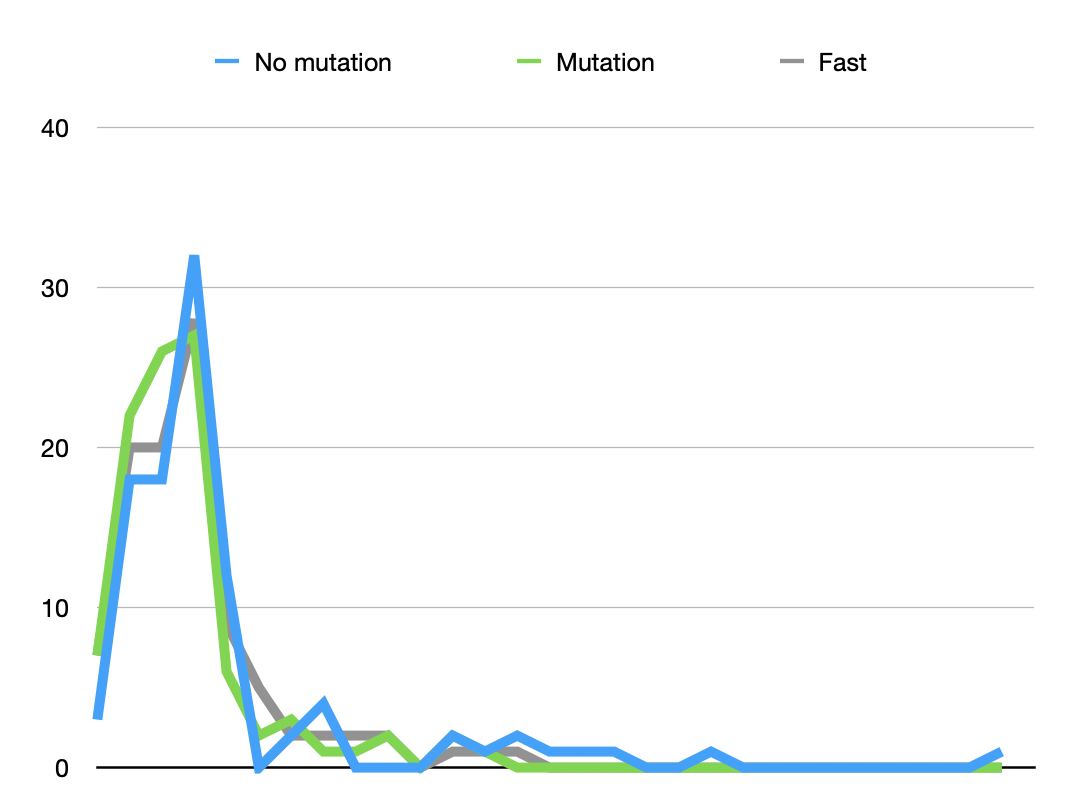
\includegraphics{Screenshot 2020-08-25 at 17.59.43.png} This is the
result of calling our data analysis program on the csv file generated by
our benchmarking program. The benchmarking program was called with those
options

\begin{Shaded}
\begin{Highlighting}[]
\NormalTok{build}\OperatorTok{/}\NormalTok{exec}\OperatorTok{/}\NormalTok{benchmarks }\OperatorTok{{-}}\NormalTok{d }\OperatorTok{../}\NormalTok{idris2}\OperatorTok{{-}}\NormalTok{fib}\OperatorTok{{-}}\NormalTok{benchmarks }\OperatorTok{{-}}\NormalTok{o results}\OperatorTok{.}\NormalTok{csv }\OperatorTok{{-}}\NormalTok{p }\OperatorTok{$}\NormalTok{(which idris2dev) }
\end{Highlighting}
\end{Shaded}

And the statistical analysis program with no options except for the
file:

\begin{Shaded}
\begin{Highlighting}[]
\NormalTok{build}\OperatorTok{/}\NormalTok{exec}\OperatorTok{/}\NormalTok{stats results\_mutation\_100\_attempts\_with\_startup}\OperatorTok{.}\NormalTok{csv}
\end{Highlighting}
\end{Shaded}

The results are in the following format:

\begin{Shaded}
\begin{Highlighting}[]
\NormalTok{name }\KeywordTok{of}\NormalTok{ benchmark, }\FunctionTok{minimum}\NormalTok{, }\FunctionTok{maximum}\NormalTok{, average, variance}
\end{Highlighting}
\end{Shaded}

The three arrays at the end correspond to an aggergation of the data in
``buckets''. Our statistical tool makes 30 ``buckets'' which represent
the different time slots that each benchmark result falls into. The
first bucket is the minimum time measured across all benchmarks and the
last bucket is the maximum time measured across all benchmarks. There
are 28 other buckets in between those two extremities. The array
represents the number of results that land for each bucket.

As you can see the results are pretty consistent with our predictions
but the values themselves aren't statistically significant. In order to
get a better picture we are going to run the same benchmark 1000 times
instead of 100.

\begin{Shaded}
\begin{Highlighting}[]
\OperatorTok{../}\DataTypeTok{Idris2\_fib\_benchmark}\OperatorTok{/}\NormalTok{fibTestNoMutation}\OperatorTok{.}\NormalTok{idr,}\FloatTok{5.08e{-}4}\NormalTok{,}\FloatTok{0.001795}\NormalTok{,}\FloatTok{6.561829999999996e{-}4}\NormalTok{,}\FloatTok{1.4789385511000005e{-}8}
\OperatorTok{../}\DataTypeTok{Idris2\_fib\_benchmark}\OperatorTok{/}\NormalTok{fibTest}\OperatorTok{.}\NormalTok{idr,}\FloatTok{5.08e{-}4}\NormalTok{,}\FloatTok{0.001753}\NormalTok{,}\FloatTok{5.882930000000001e{-}4}\NormalTok{,}\FloatTok{1.5392219150999998e{-}8}
\OperatorTok{../}\DataTypeTok{Idris2\_fib\_benchmark}\OperatorTok{/}\NormalTok{fibTailRec}\OperatorTok{.}\NormalTok{idr,}\FloatTok{4.89e{-}4}\NormalTok{,}\FloatTok{0.001974}\NormalTok{,}\FloatTok{6.241300000000006e{-}4}\NormalTok{,}\FloatTok{3.8718697099999886e{-}8}

\NormalTok{[}\DecValTok{53}\NormalTok{, }\DecValTok{126}\NormalTok{, }\DecValTok{460}\NormalTok{, }\DecValTok{192}\NormalTok{, }\DecValTok{47}\NormalTok{, }\DecValTok{23}\NormalTok{, }\DecValTok{31}\NormalTok{, }\DecValTok{32}\NormalTok{, }\DecValTok{11}\NormalTok{, }\DecValTok{5}\NormalTok{, }\DecValTok{1}\NormalTok{, }\DecValTok{2}\NormalTok{, }\DecValTok{2}\NormalTok{, }\DecValTok{4}\NormalTok{, }\DecValTok{1}\NormalTok{, }\DecValTok{5}\NormalTok{, }\DecValTok{0}\NormalTok{, }\DecValTok{2}\NormalTok{, }\DecValTok{1}\NormalTok{, }\DecValTok{1}\NormalTok{, }\DecValTok{0}\NormalTok{, }\DecValTok{0}\NormalTok{, }\DecValTok{0}\NormalTok{, }\DecValTok{0}\NormalTok{, }\DecValTok{0}\NormalTok{, }\DecValTok{1}\NormalTok{, }\DecValTok{0}\NormalTok{, }\DecValTok{0}\NormalTok{, }\DecValTok{0}\NormalTok{, }\DecValTok{0}\NormalTok{]}
\NormalTok{[}\DecValTok{261}\NormalTok{, }\DecValTok{546}\NormalTok{, }\DecValTok{76}\NormalTok{, }\DecValTok{32}\NormalTok{, }\DecValTok{18}\NormalTok{, }\DecValTok{12}\NormalTok{, }\DecValTok{13}\NormalTok{, }\DecValTok{7}\NormalTok{, }\DecValTok{2}\NormalTok{, }\DecValTok{5}\NormalTok{, }\DecValTok{10}\NormalTok{, }\DecValTok{4}\NormalTok{, }\DecValTok{3}\NormalTok{, }\DecValTok{5}\NormalTok{, }\DecValTok{0}\NormalTok{, }\DecValTok{1}\NormalTok{, }\DecValTok{1}\NormalTok{, }\DecValTok{0}\NormalTok{, }\DecValTok{0}\NormalTok{, }\DecValTok{2}\NormalTok{, }\DecValTok{0}\NormalTok{, }\DecValTok{1}\NormalTok{, }\DecValTok{0}\NormalTok{, }\DecValTok{0}\NormalTok{, }\DecValTok{1}\NormalTok{, }\DecValTok{0}\NormalTok{, }\DecValTok{0}\NormalTok{, }\DecValTok{0}\NormalTok{, }\DecValTok{0}\NormalTok{, }\DecValTok{0}\NormalTok{]}
\NormalTok{[}\DecValTok{217}\NormalTok{, }\DecValTok{527}\NormalTok{, }\DecValTok{80}\NormalTok{, }\DecValTok{44}\NormalTok{, }\DecValTok{23}\NormalTok{, }\DecValTok{14}\NormalTok{, }\DecValTok{12}\NormalTok{, }\DecValTok{11}\NormalTok{, }\DecValTok{7}\NormalTok{, }\DecValTok{6}\NormalTok{, }\DecValTok{10}\NormalTok{, }\DecValTok{2}\NormalTok{, }\DecValTok{6}\NormalTok{, }\DecValTok{11}\NormalTok{, }\DecValTok{5}\NormalTok{, }\DecValTok{4}\NormalTok{, }\DecValTok{4}\NormalTok{, }\DecValTok{2}\NormalTok{, }\DecValTok{1}\NormalTok{, }\DecValTok{2}\NormalTok{, }\DecValTok{1}\NormalTok{, }\DecValTok{1}\NormalTok{, }\DecValTok{0}\NormalTok{, }\DecValTok{3}\NormalTok{, }\DecValTok{3}\NormalTok{, }\DecValTok{1}\NormalTok{, }\DecValTok{2}\NormalTok{, }\DecValTok{0}\NormalTok{, }\DecValTok{0}\NormalTok{, }\DecValTok{1}\NormalTok{]}
\end{Highlighting}
\end{Shaded}

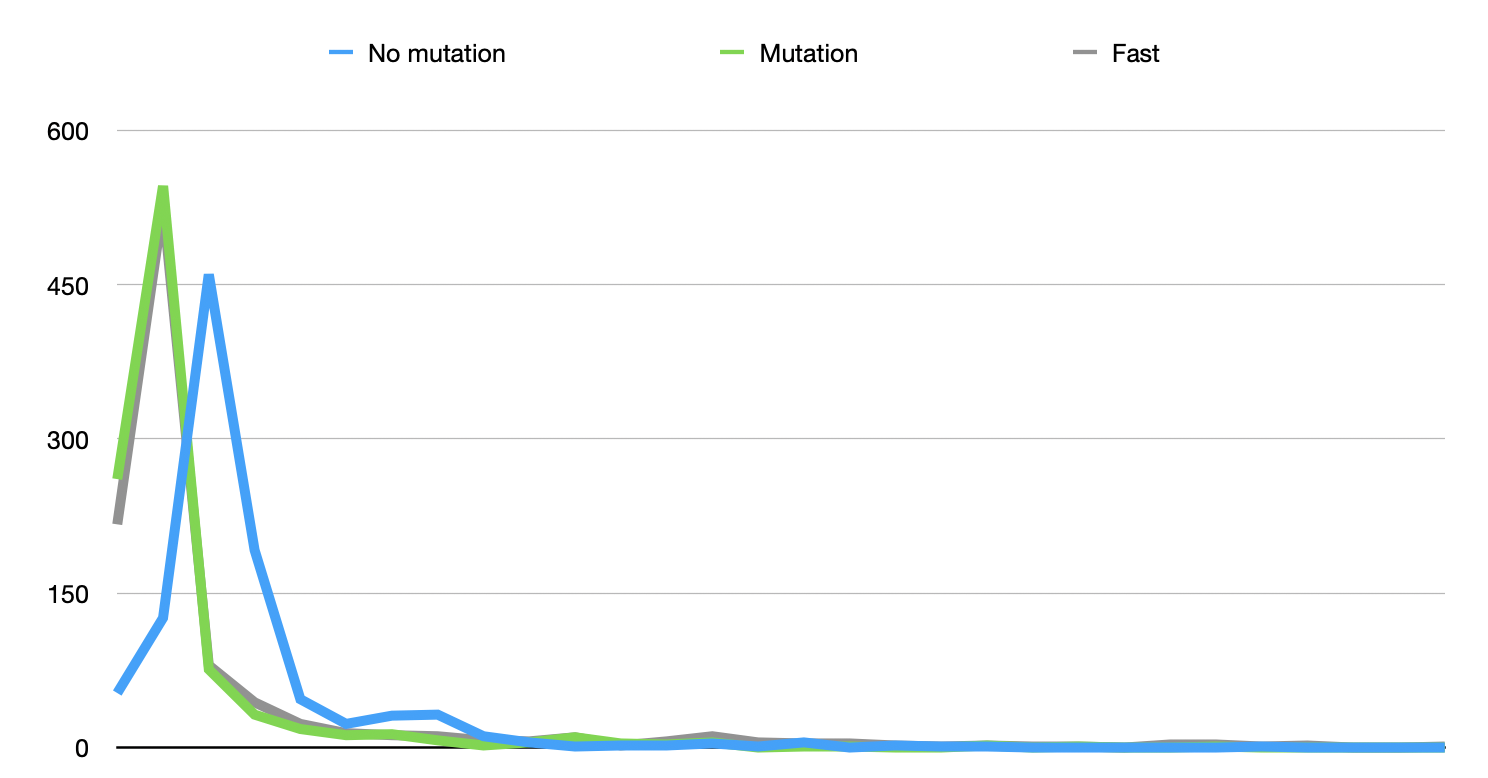
\includegraphics{Screenshot 2020-08-25 at 18.00.17.png} The results are
pretty similar which gives us a greater confidence in their accuracy.

There is however something we can do to improve our measurement and that
is to subtract the startup time of the scheme runtime. Indeed every
program is measured using the difference between the time it started and
the time it ended. But this time also includes the time it takes to
launch scheme and then execute a program on it. Indeed the following
program:

\begin{Shaded}
\begin{Highlighting}[]
\NormalTok{main }\OperatorTok{:} \DataTypeTok{IO}\NormalTok{ ()}
\NormalTok{main }\OtherTok{=} \FunctionTok{pure}\NormalTok{ ()}
\end{Highlighting}
\end{Shaded}

Takes 0.13 seconds to run despite doing nothing. This time is the
startup time and can go up to 0.3 seconds.

\hypertarget{results-2-fibonacci-without-startup-time}{%
\subsection{Results 2: Fibonacci without startup
time}\label{results-2-fibonacci-without-startup-time}}

In order to remove the startup time we are going to change the emitted
bytecode to wrap our main function inside a time-measuring function.
Since the timer won't start until the program is ready to run the
startup time will be eliminated. Running our empty program we get

\begin{Shaded}
\begin{Highlighting}[]
\FloatTok{0.000000000}\NormalTok{s elapsed cpu time}
\end{Highlighting}
\end{Shaded}

Which is what we expect.

This time we will run our benchmarks 1000 times using the same command
as before. We expect to see the same results but the difference should
give us a greater interval of confidence. Running our statistical
analysis gives us those results

\begin{Shaded}
\begin{Highlighting}[]
\OperatorTok{../}\DataTypeTok{Idris2\_fib\_benchmark}\OperatorTok{/}\NormalTok{fibTestNoMutation}\OperatorTok{.}\NormalTok{idr,}\FloatTok{1.696760896}\NormalTok{,}\FloatTok{1.977075901}\NormalTok{,}\FloatTok{1.7447377120060026}\NormalTok{,}\FloatTok{9.18303221644259e{-}4}
\OperatorTok{../}\DataTypeTok{Idris2\_fib\_benchmark}\OperatorTok{/}\NormalTok{fibTest}\OperatorTok{.}\NormalTok{idr,}\FloatTok{1.734708117}\NormalTok{,}\FloatTok{2.152951106}\NormalTok{,}\FloatTok{1.786299514231}\NormalTok{,}\FloatTok{0.002247060292357963}
\OperatorTok{../}\DataTypeTok{Idris2\_fib\_benchmark}\OperatorTok{/}\NormalTok{fibTailRec}\OperatorTok{.}\NormalTok{idr,}\FloatTok{1.65627213}\NormalTok{,}\FloatTok{1.881412963}\NormalTok{,}\FloatTok{1.6768551703740004}\NormalTok{,}\FloatTok{9.142437018832634e{-}4}

\NormalTok{[}\DecValTok{0}\NormalTok{, }\DecValTok{0}\NormalTok{, }\DecValTok{136}\NormalTok{, }\DecValTok{113}\NormalTok{, }\DecValTok{17}\NormalTok{, }\DecValTok{620}\NormalTok{, }\DecValTok{62}\NormalTok{, }\DecValTok{22}\NormalTok{, }\DecValTok{4}\NormalTok{, }\DecValTok{6}\NormalTok{, }\DecValTok{4}\NormalTok{, }\DecValTok{3}\NormalTok{, }\DecValTok{2}\NormalTok{, }\DecValTok{3}\NormalTok{, }\DecValTok{4}\NormalTok{, }\DecValTok{0}\NormalTok{, }\DecValTok{1}\NormalTok{, }\DecValTok{2}\NormalTok{, }\DecValTok{1}\NormalTok{, }\DecValTok{0}\NormalTok{, }\DecValTok{0}\NormalTok{, }\DecValTok{0}\NormalTok{, }\DecValTok{0}\NormalTok{, }\DecValTok{0}\NormalTok{, }\DecValTok{0}\NormalTok{, }\DecValTok{0}\NormalTok{, }\DecValTok{0}\NormalTok{, }\DecValTok{0}\NormalTok{, }\DecValTok{0}\NormalTok{, }\DecValTok{0}\NormalTok{]}
\NormalTok{[}\DecValTok{0}\NormalTok{, }\DecValTok{0}\NormalTok{, }\DecValTok{0}\NormalTok{, }\DecValTok{0}\NormalTok{, }\DecValTok{164}\NormalTok{, }\DecValTok{217}\NormalTok{, }\DecValTok{36}\NormalTok{, }\DecValTok{160}\NormalTok{, }\DecValTok{264}\NormalTok{, }\DecValTok{47}\NormalTok{, }\DecValTok{36}\NormalTok{, }\DecValTok{18}\NormalTok{, }\DecValTok{19}\NormalTok{, }\DecValTok{7}\NormalTok{, }\DecValTok{5}\NormalTok{, }\DecValTok{5}\NormalTok{, }\DecValTok{7}\NormalTok{, }\DecValTok{3}\NormalTok{, }\DecValTok{2}\NormalTok{, }\DecValTok{3}\NormalTok{, }\DecValTok{2}\NormalTok{, }\DecValTok{2}\NormalTok{, }\DecValTok{1}\NormalTok{, }\DecValTok{0}\NormalTok{, }\DecValTok{0}\NormalTok{, }\DecValTok{0}\NormalTok{, }\DecValTok{1}\NormalTok{, }\DecValTok{0}\NormalTok{, }\DecValTok{0}\NormalTok{, }\DecValTok{1}\NormalTok{]}
\NormalTok{[}\DecValTok{647}\NormalTok{, }\DecValTok{221}\NormalTok{, }\DecValTok{19}\NormalTok{, }\DecValTok{4}\NormalTok{, }\DecValTok{52}\NormalTok{, }\DecValTok{33}\NormalTok{, }\DecValTok{8}\NormalTok{, }\DecValTok{2}\NormalTok{, }\DecValTok{5}\NormalTok{, }\DecValTok{2}\NormalTok{, }\DecValTok{0}\NormalTok{, }\DecValTok{4}\NormalTok{, }\DecValTok{2}\NormalTok{, }\DecValTok{1}\NormalTok{, }\DecValTok{0}\NormalTok{, }\DecValTok{0}\NormalTok{, }\DecValTok{0}\NormalTok{, }\DecValTok{0}\NormalTok{, }\DecValTok{0}\NormalTok{, }\DecValTok{0}\NormalTok{, }\DecValTok{0}\NormalTok{, }\DecValTok{0}\NormalTok{, }\DecValTok{0}\NormalTok{, }\DecValTok{0}\NormalTok{, }\DecValTok{0}\NormalTok{, }\DecValTok{0}\NormalTok{, }\DecValTok{0}\NormalTok{, }\DecValTok{0}\NormalTok{, }\DecValTok{0}\NormalTok{, }\DecValTok{0}\NormalTok{]}
\end{Highlighting}
\end{Shaded}

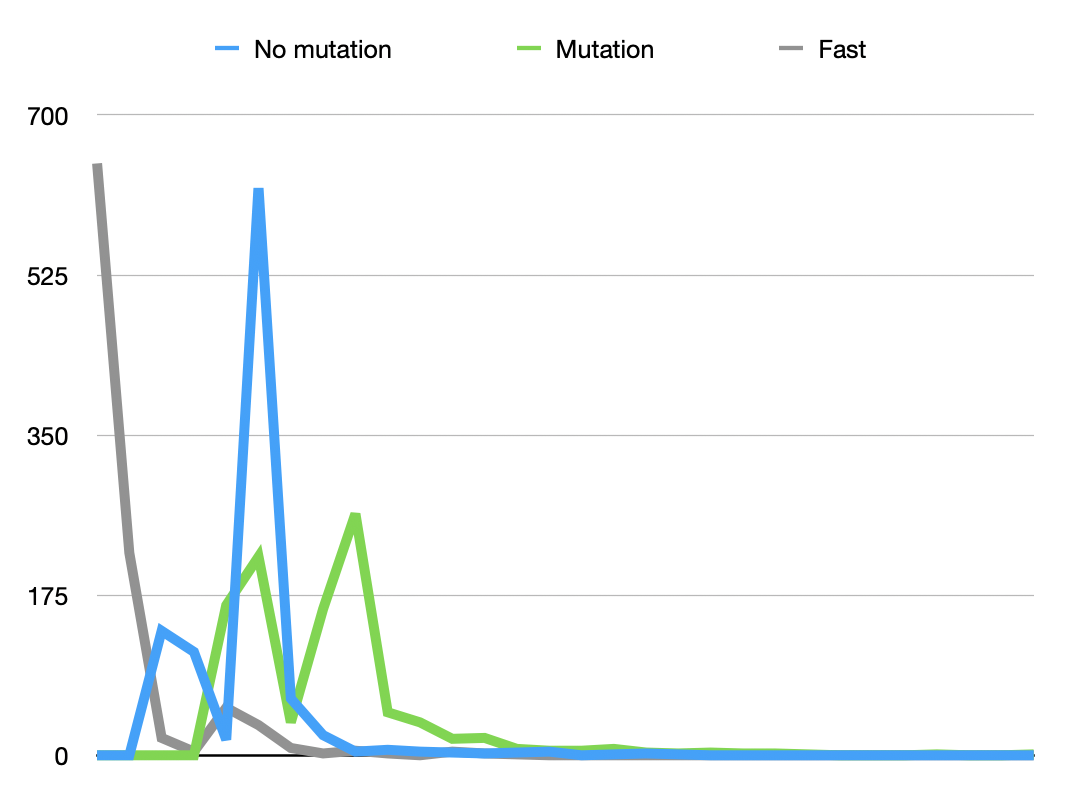
\includegraphics{Screenshot 2020-08-25 at 17.59.34.png} As you can see
the results aren't exactly as expected, both our \emph{average} and our
\emph{variance} is higher than without any optimisation. A result that
we definitely did not anticipate and goes against the belief that
founded our hypothesis.

One possible explanation is that scheme performs JIT compilation and
correctly identifies the hot-loop in our unoptimized example but is
unable to perform such optimization with our mix of pure and mutating
code.

\hypertarget{results-3-fibonacci-without-startup-time-small-loop}{%
\subsection{Results 3: Fibonacci without startup time, small
loop}\label{results-3-fibonacci-without-startup-time-small-loop}}

In order to test the JIT hypothesis we are going to run the same test,
\emph{without} startup time but with a much smaller loop so that the
results are measured in milliseconds rather than seconds. This should be
enough to prevent the runtime from identifying the loop and performing
its optimisation.

In order to reduce the running time from seconds to milliseconds we
simply change the loop count from \texttt{8*10\^{}6} to
\texttt{8*10\^{}4} reducing it by two orders of magnitude reduces the
running time accordingly.

\begin{Shaded}
\begin{Highlighting}[]
\OperatorTok{../}\DataTypeTok{Idris2\_fib\_benchmark}\OperatorTok{/}\NormalTok{fibTestNoMutation}\OperatorTok{.}\NormalTok{idr,}\FloatTok{0.007216185}\NormalTok{,}\FloatTok{0.008861124}\NormalTok{,}\FloatTok{0.007520532116999987}\NormalTok{,}\FloatTok{3.5827851856347296e{-}8}
\OperatorTok{../}\DataTypeTok{Idris2\_fib\_benchmark}\OperatorTok{/}\NormalTok{fibTest}\OperatorTok{.}\NormalTok{idr,}\FloatTok{0.006543267}\NormalTok{,}\FloatTok{0.010942671}\NormalTok{,}\FloatTok{0.006867369243000004}\NormalTok{,}\FloatTok{5.3106313711037986e{-}8}
\OperatorTok{../}\DataTypeTok{Idris2\_fib\_benchmark}\OperatorTok{/}\NormalTok{fibTailRec}\OperatorTok{.}\NormalTok{idr,}\FloatTok{0.006385357}\NormalTok{,}\FloatTok{0.007625528}\NormalTok{,}\FloatTok{0.006624731209000001}\NormalTok{,}\FloatTok{2.4002041892751334e{-}8}

\NormalTok{[}\DecValTok{0}\NormalTok{, }\DecValTok{0}\NormalTok{, }\DecValTok{0}\NormalTok{, }\DecValTok{0}\NormalTok{, }\DecValTok{0}\NormalTok{, }\DecValTok{72}\NormalTok{, }\DecValTok{411}\NormalTok{, }\DecValTok{361}\NormalTok{, }\DecValTok{106}\NormalTok{, }\DecValTok{17}\NormalTok{, }\DecValTok{12}\NormalTok{, }\DecValTok{8}\NormalTok{, }\DecValTok{6}\NormalTok{, }\DecValTok{2}\NormalTok{, }\DecValTok{3}\NormalTok{, }\DecValTok{2}\NormalTok{, }\DecValTok{0}\NormalTok{, }\DecValTok{0}\NormalTok{, }\DecValTok{0}\NormalTok{, }\DecValTok{0}\NormalTok{, }\DecValTok{0}\NormalTok{, }\DecValTok{0}\NormalTok{, }\DecValTok{0}\NormalTok{, }\DecValTok{0}\NormalTok{, }\DecValTok{0}\NormalTok{, }\DecValTok{0}\NormalTok{, }\DecValTok{0}\NormalTok{, }\DecValTok{0}\NormalTok{, }\DecValTok{0}\NormalTok{, }\DecValTok{0}\NormalTok{]}
\NormalTok{[}\DecValTok{0}\NormalTok{, }\DecValTok{95}\NormalTok{, }\DecValTok{493}\NormalTok{, }\DecValTok{288}\NormalTok{, }\DecValTok{83}\NormalTok{, }\DecValTok{13}\NormalTok{, }\DecValTok{9}\NormalTok{, }\DecValTok{10}\NormalTok{, }\DecValTok{3}\NormalTok{, }\DecValTok{0}\NormalTok{, }\DecValTok{3}\NormalTok{, }\DecValTok{1}\NormalTok{, }\DecValTok{0}\NormalTok{, }\DecValTok{0}\NormalTok{, }\DecValTok{0}\NormalTok{, }\DecValTok{0}\NormalTok{, }\DecValTok{0}\NormalTok{, }\DecValTok{0}\NormalTok{, }\DecValTok{1}\NormalTok{, }\DecValTok{0}\NormalTok{, }\DecValTok{0}\NormalTok{, }\DecValTok{0}\NormalTok{, }\DecValTok{0}\NormalTok{, }\DecValTok{0}\NormalTok{, }\DecValTok{0}\NormalTok{, }\DecValTok{0}\NormalTok{, }\DecValTok{0}\NormalTok{, }\DecValTok{0}\NormalTok{, }\DecValTok{0}\NormalTok{, }\DecValTok{1}\NormalTok{]}
\NormalTok{[}\DecValTok{303}\NormalTok{, }\DecValTok{470}\NormalTok{, }\DecValTok{161}\NormalTok{, }\DecValTok{41}\NormalTok{, }\DecValTok{13}\NormalTok{, }\DecValTok{7}\NormalTok{, }\DecValTok{1}\NormalTok{, }\DecValTok{4}\NormalTok{, }\DecValTok{0}\NormalTok{, }\DecValTok{0}\NormalTok{, }\DecValTok{0}\NormalTok{, }\DecValTok{0}\NormalTok{, }\DecValTok{0}\NormalTok{, }\DecValTok{0}\NormalTok{, }\DecValTok{0}\NormalTok{, }\DecValTok{0}\NormalTok{, }\DecValTok{0}\NormalTok{, }\DecValTok{0}\NormalTok{, }\DecValTok{0}\NormalTok{, }\DecValTok{0}\NormalTok{, }\DecValTok{0}\NormalTok{, }\DecValTok{0}\NormalTok{, }\DecValTok{0}\NormalTok{, }\DecValTok{0}\NormalTok{, }\DecValTok{0}\NormalTok{, }\DecValTok{0}\NormalTok{, }\DecValTok{0}\NormalTok{, }\DecValTok{0}\NormalTok{, }\DecValTok{0}\NormalTok{, }\DecValTok{0}\NormalTok{]}
\end{Highlighting}
\end{Shaded}

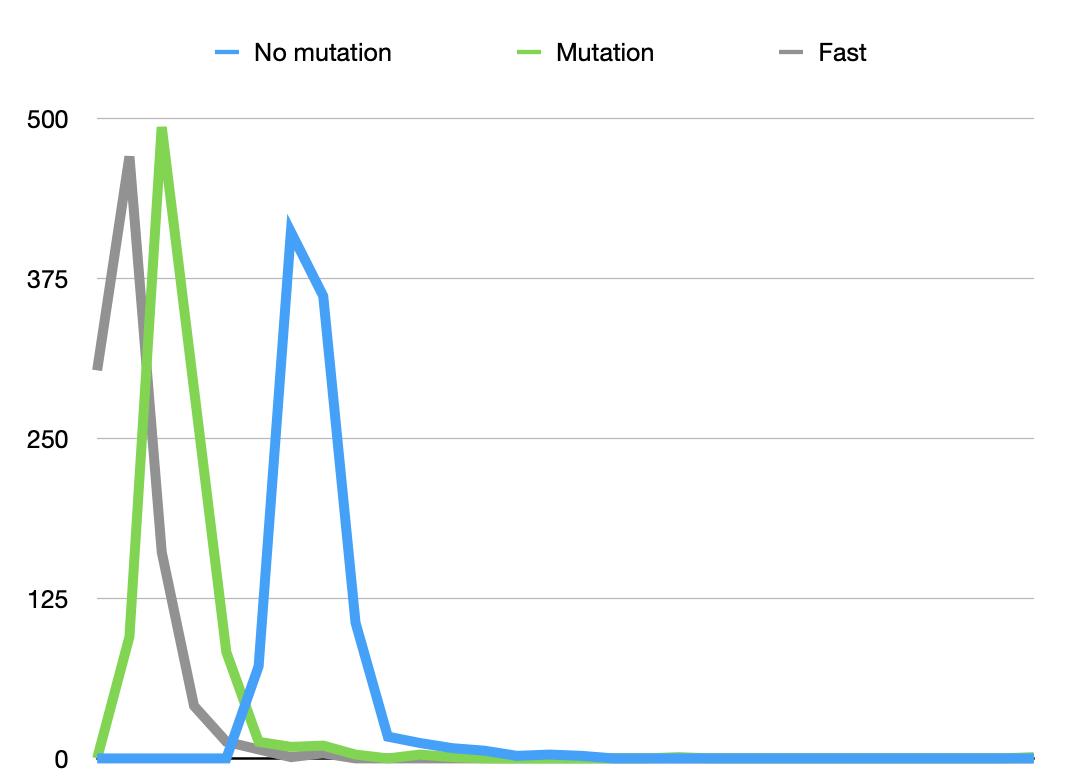
\includegraphics{Screenshot 2020-08-25 at 17.59.21.png} And indeed this
data does not disprove our JIT hypothesis (but it does not confirm it
either). However, since this thesis is not about the intricacies of the
scheme runtime we are going to let the issue rest for now.

Those results showcase two things: That our optimisation works, and that
it is not significant enough to be strictly superior to other forms of
optimisations. Ideally the best way to test our optimisation would be to
write our own runtime which runs on \emph{bare metal} or some
approximation of it (WASM/LLVM) which would (probably) be even faster
than scheme, and give us more control over which optimisations play
nicely together and which ones are redundant or even harmful to
performance.

Idris2 has an alternative javascript backend, however, the javascript
code generation is unable to translate our programs into plain loops
free of recursion. Because of this, our benchmark exceeds the maximum
stack size and the program aborts. When the stack size is increased the
program segfaults.

\hypertarget{safe-inlining}{%
\section{Safe inlining}\label{safe-inlining}}

As we've seen in the context review, one of the use-cases for linear
types is to detect where control flow allows for safe inlining of
functions. In the following snippet, \texttt{y} cannot be inlined
without duplicating computation.

\begin{Shaded}
\begin{Highlighting}[]
\KeywordTok{let}\NormalTok{ x }\OtherTok{=} \DecValTok{1} \OperatorTok{+} \DecValTok{2}
\NormalTok{    y }\OtherTok{=}\NormalTok{ x }\OperatorTok{+} \DecValTok{3} \KeywordTok{in}
\NormalTok{    y }\OperatorTok{+}\NormalTok{ y}
\end{Highlighting}
\end{Shaded}

Indeed inlining it would result in

\begin{Shaded}
\begin{Highlighting}[]
\KeywordTok{let}\NormalTok{ x }\OtherTok{=} \DecValTok{1} \OperatorTok{+} \DecValTok{2}
\NormalTok{    x }\OperatorTok{+} \DecValTok{3} \OperatorTok{+}\NormalTok{ x }\OperatorTok{+} \DecValTok{3}
\end{Highlighting}
\end{Shaded}

where the \texttt{+\ 3} operation is performed twice. \texttt{x} however
can be inlined safely:

\begin{Shaded}
\begin{Highlighting}[]
\KeywordTok{let}\NormalTok{ y }\OtherTok{=} \DecValTok{1} \OperatorTok{+} \DecValTok{2} \OperatorTok{+} \DecValTok{3} \KeywordTok{in}
\NormalTok{    y }\OperatorTok{+}\NormalTok{ y}
\end{Highlighting}
\end{Shaded}

the \texttt{1\ +\ 2} operation is performed only once after inlining.

One area where linearity and inlining comes into play is when defining
effects. Indeed, a linear state monad could have the following
\texttt{bind} signature:

\begin{Shaded}
\begin{Highlighting}[]
\NormalTok{(}\OperatorTok{\textgreater{}\textgreater{}=}\NormalTok{) }\OperatorTok{:}\NormalTok{ (}\DecValTok{1}\NormalTok{ \_ }\OperatorTok{:} \DataTypeTok{LState}\NormalTok{ s a) }\OtherTok{{-}\textgreater{}}\NormalTok{ (}\DecValTok{1}\NormalTok{ f }\OperatorTok{:}\NormalTok{ a }\OtherTok{{-}\textgreater{}} \DataTypeTok{LState}\NormalTok{ s b) }\OtherTok{{-}\textgreater{}} \DataTypeTok{LState}\NormalTok{ s b}
\NormalTok{(}\OperatorTok{\textgreater{}\textgreater{}=}\NormalTok{) (}\DataTypeTok{LState}\NormalTok{ s) c }\OtherTok{=} \DataTypeTok{LState}\NormalTok{ (\textbackslash{}x }\OtherTok{=\textgreater{}}\NormalTok{ …)}
\end{Highlighting}
\end{Shaded}

Which indicates that the state is inspected linearity and the function
is applied exactly once. Since programs using \texttt{bind} compose with
themselves we often see the following sequence of operations:

\begin{Shaded}
\begin{Highlighting}[]
\NormalTok{inital }\OperatorTok{\textgreater{}\textgreater{}=}\NormalTok{ f }\OperatorTok{\textgreater{}\textgreater{}=}\NormalTok{ g}
\end{Highlighting}
\end{Shaded}

which once inlined results in

\begin{Shaded}
\begin{Highlighting}[]
\DataTypeTok{LState}\NormalTok{ (\textbackslash{}x }\OtherTok{=\textgreater{}} \KeywordTok{let}\NormalTok{ v }\OtherTok{=}\NormalTok{ initial }\OperatorTok{\textgreater{}\textgreater{}=}\NormalTok{ f)}
\NormalTok{                  g v)}
\end{Highlighting}
\end{Shaded}

\begin{Shaded}
\begin{Highlighting}[]
\DataTypeTok{LState}\NormalTok{ (\textbackslash{}x }\OtherTok{=\textgreater{}} \KeywordTok{let}\NormalTok{ v }\OtherTok{=}\NormalTok{ x (}\DataTypeTok{LState}\NormalTok{ (\textbackslash{}y }\OtherTok{=\textgreater{}} \KeywordTok{let}\NormalTok{ w }\OtherTok{=}\NormalTok{ y initial }
\NormalTok{                                           f w))}
\NormalTok{                  g v)}
\end{Highlighting}
\end{Shaded}

\hypertarget{future-work}{%
\section{Future work}\label{future-work}}

\hypertarget{enlarging-the-scope}{%
\subsection{Enlarging the scope}\label{enlarging-the-scope}}

Currently we only look at the \emph{immediate} scope of let bindings.
Technically speaking there is nothing preventing our optimisation from
working with a more indirect scoping mechanism. Indeed the following
should trigger our optimisation

\begin{Shaded}
\begin{Highlighting}[]
\NormalTok{defaultVal }\OperatorTok{:} \DataTypeTok{MyData}
\NormalTok{defaultVal }\OtherTok{=} \DataTypeTok{MkDefault} \DecValTok{3}

\NormalTok{update }\OperatorTok{:}\NormalTok{ (}\DecValTok{1}\NormalTok{ rec }\OperatorTok{:} \DataTypeTok{MyData}\NormalTok{) }\OtherTok{{-}\textgreater{}} \DataTypeTok{MyData}
\NormalTok{update (}\DataTypeTok{MkDefault}\NormalTok{ n) }\OtherTok{=} \DataTypeTok{MkDefault}\NormalTok{ (}\DataTypeTok{S}\NormalTok{ n)}
\NormalTok{update (}\DataTypeTok{MkOther}\NormalTok{ n) }\OtherTok{=} \DataTypeTok{MkOther}\NormalTok{ (}\DataTypeTok{S}\NormalTok{ (}\DataTypeTok{S}\NormalTok{ n))}

\NormalTok{operate }\OperatorTok{:} \DataTypeTok{MyData}
\NormalTok{operate }\OtherTok{=} \KeywordTok{let} \DecValTok{1}\NormalTok{ def }\OtherTok{=}\NormalTok{ defaultVal}
              \DecValTok{1}\NormalTok{ newVal }\OtherTok{=}\NormalTok{ update def }\KeywordTok{in}
\NormalTok{              update newVal}
\end{Highlighting}
\end{Shaded}

But it will not because \texttt{defaultVal} is not a constructor, it's a
function call that returns itself a constructor.

One implementation strategy would be to wait for the compiler to inline
those definitions and then run our optimiser without further changes.

Another optimisation would be to aggressively follow references to see
if they result in plain data constructors and replace the entire call
chain by the constructor itself, and then run our optimisation.

While both those strategies are valid they incur a cost in terms of
complexity and compile time that may not be worth the effort in terms of
performance results. They could be hidden behind a -O3 flag, but that
kind of effort is probably better spend in making the ergonomics of
linear types more streamlined, which would help make those optimisations
more commonplace. Which is the topic of the next section

\hypertarget{making-linearity-easier-to-use}{%
\subsection{Making linearity easier to
use}\label{making-linearity-easier-to-use}}

There are multiple barriers that make linearity harder to use than one
might expect. They roughly end up in two buckets:

\begin{itemize}
\tightlist
\item
  I want to use linearity but I cannot
\item
  I have a linear variable and that's actually annoying
\end{itemize}

\hypertarget{not-linear-enough}{%
\subsubsection{Not linear enough}\label{not-linear-enough}}

The first one appears when the programmer tries to make thoughtful usage
of linear and erased annotation but finds that other parts of existing
libraries do not support linearity. Here are a couple of examples

\begin{Shaded}
\begin{Highlighting}[]
\NormalTok{operate }\OperatorTok{:}\NormalTok{ (}\DecValTok{1}\NormalTok{ n }\OperatorTok{:} \DataTypeTok{Nat}\NormalTok{) }\OtherTok{{-}\textgreater{}}\NormalTok{ (}\DecValTok{1}\NormalTok{ m }\OperatorTok{:} \DataTypeTok{Nat}\NormalTok{) }\OtherTok{{-}\textgreater{}} \DataTypeTok{Int}
\NormalTok{operate n m }\OtherTok{=}\NormalTok{ n }\OperatorTok{+}\NormalTok{ m}
\end{Highlighting}
\end{Shaded}

gives the error

\begin{Shaded}
\begin{Highlighting}[]
\DataTypeTok{Trying}\NormalTok{ to use linear name n }\KeywordTok{in}\NormalTok{ non}\OperatorTok{{-}}\NormalTok{linear context}
\end{Highlighting}
\end{Shaded}

Because the \texttt{+} interface is defined as

\begin{Shaded}
\begin{Highlighting}[]
\NormalTok{interface }\DataTypeTok{Num}\NormalTok{ ty }\KeywordTok{where}
\NormalTok{    (}\OperatorTok{+}\NormalTok{) }\OperatorTok{:}\NormalTok{ ty }\OtherTok{{-}\textgreater{}}\NormalTok{ ty }\OtherTok{{-}\textgreater{}}\NormalTok{ ty}
\end{Highlighting}
\end{Shaded}

Despite addition on \texttt{Nat} being defined linearly

\begin{Shaded}
\begin{Highlighting}[]
\NormalTok{plus }\OperatorTok{:}\NormalTok{ (}\DecValTok{1}\NormalTok{ n }\OperatorTok{:} \DataTypeTok{Nat}\NormalTok{) }\OtherTok{{-}\textgreater{}}\NormalTok{ (}\DecValTok{1}\NormalTok{ m }\OperatorTok{:} \DataTypeTok{Nat}\NormalTok{) }\OtherTok{{-}\textgreater{}} \DataTypeTok{Nat}
\NormalTok{plus }\DataTypeTok{Z}\NormalTok{ m }\OtherTok{=}\NormalTok{ m}
\NormalTok{plus (}\DataTypeTok{S}\NormalTok{ n) m }\OtherTok{=} \DataTypeTok{S}\NormalTok{ (plus n m)}
\end{Highlighting}
\end{Shaded}

A similar problem occurs with interfaces

\begin{Shaded}
\begin{Highlighting}[]
\NormalTok{interface }\DataTypeTok{Monad}\NormalTok{ (}\DataTypeTok{Type} \OtherTok{{-}\textgreater{}} \DataTypeTok{Type}\NormalTok{) }\KeywordTok{where}
    \OperatorTok{...}

\KeywordTok{data} \DataTypeTok{MyData} \OperatorTok{:}\NormalTok{ (}\DecValTok{0}\NormalTok{ ty }\OperatorTok{:} \DataTypeTok{Type}\NormalTok{) }\OtherTok{{-}\textgreater{}} \DataTypeTok{Type} \KeywordTok{where}
    \OperatorTok{...}

\KeywordTok{instance} \DataTypeTok{Monad} \DataTypeTok{MyData} \KeywordTok{where}
    \OperatorTok{...}
\end{Highlighting}
\end{Shaded}

\begin{Shaded}
\begin{Highlighting}[]
\DataTypeTok{Expected} \DataTypeTok{Type} \OtherTok{{-}\textgreater{}} \DataTypeTok{Type}
\NormalTok{got (}\DecValTok{0}\NormalTok{ ty }\OperatorTok{:} \DataTypeTok{Type}\NormalTok{) }\OtherTok{{-}\textgreater{}} \DataTypeTok{Type}
\end{Highlighting}
\end{Shaded}

One way to solve those issues would be to have linearity polymorphism
and be able to abstract over linearity annotations. For example the map
function could be written as

\begin{Shaded}
\begin{Highlighting}[]
\FunctionTok{map} \OperatorTok{:} \KeywordTok{forall}\NormalTok{ l }\OperatorTok{.}\NormalTok{ ((l v }\OperatorTok{:}\NormalTok{ a) }\OtherTok{{-}\textgreater{}}\NormalTok{ b) }\OtherTok{{-}\textgreater{}}\NormalTok{ (l ls }\OperatorTok{:} \DataTypeTok{List}\NormalTok{ a) }\OtherTok{{-}\textgreater{}} \DataTypeTok{List}\NormalTok{ b}
\FunctionTok{map}\NormalTok{ f [] }\OtherTok{=}\NormalTok{ []}
\FunctionTok{map}\NormalTok{ f (}\OtherTok{x ::}\NormalTok{ xs) }\OtherTok{=}\NormalTok{ f}\OtherTok{ x ::} \FunctionTok{map}\NormalTok{ f xs}
\end{Highlighting}
\end{Shaded}

That is, the list is linearly consumed iff the higher order function is
linear. What it means for our interface problem is that it could be
rewritten as

\begin{Shaded}
\begin{Highlighting}[]
\NormalTok{interface }\KeywordTok{forall}\NormalTok{ l }\OperatorTok{.} \DataTypeTok{Functor}\NormalTok{ (m }\OperatorTok{:}\NormalTok{ (l \_ }\OperatorTok{:} \DataTypeTok{Type}\NormalTok{) }\OtherTok{{-}\textgreater{}} \DataTypeTok{Type}\NormalTok{) }\KeywordTok{where}
    \OperatorTok{...}
\NormalTok{interface }\KeywordTok{forall}\NormalTok{ l }\OperatorTok{.} \DataTypeTok{Functor}\NormalTok{ \{l\} m }\OtherTok{⇒} \DataTypeTok{Applicative}\NormalTok{ \{l\} m }\KeywordTok{where}
    \OperatorTok{...}
\NormalTok{interface }\KeywordTok{forall}\NormalTok{ l }\OperatorTok{.} \DataTypeTok{Applicative}\NormalTok{ \{l\} m }\OtherTok{⇒} \DataTypeTok{Monad}\NormalTok{ \{l\} m }\KeywordTok{where}
    \OperatorTok{...}
\end{Highlighting}
\end{Shaded}

A similar solution could be provided for \texttt{Num}

\begin{Shaded}
\begin{Highlighting}[]
\NormalTok{interface }\DataTypeTok{Num}\NormalTok{ ty }\KeywordTok{where}
\NormalTok{    (}\OperatorTok{+}\NormalTok{) }\OperatorTok{:} \KeywordTok{forall}\NormalTok{ l}\OperatorTok{.}\NormalTok{ (l n }\OperatorTok{:}\NormalTok{ ty) }\OtherTok{{-}\textgreater{}}\NormalTok{ (l m }\OperatorTok{:}\NormalTok{ ty) }\OtherTok{{-}\textgreater{}}\NormalTok{ ty}
\end{Highlighting}
\end{Shaded}

So that it can be used with both linear and non-linear variables.

\hypertarget{too-linear-now} linear in every aspect. We also
mentioned how this is a problem to implement basic functionality like
\texttt{drop} and \texttt{copy}, but those are artifical examples,
rarely does a programmer need to call \texttt{copy} or \texttt{drop} in
industrial applications. Therefore I will present a couple of situation
where being \emph{entirely} linear results in tricky code or impossible
code and then propose a solution.

\hypertarget{logging}{%
\paragraph{Logging}\label{logging}}

This is a common scenario, you're trying to debug effectful code, and
for this you're spreading around log statements hoping that running the
program will give you insight into how it's running.

\begin{Shaded}
\begin{Highlighting}[]
\KeywordTok{do}\NormalTok{ datas }\OtherTok{\textless{}{-}}\NormalTok{ getData arg1 arg2}
   \DataTypeTok{Just}\NormalTok{ success }\OtherTok{\textless{}{-}}\NormalTok{ trySomething datas (options}\OperatorTok{.}\NormalTok{memoized)}
     \OperatorTok{|}\NormalTok{ \_ }\OtherTok{⇒} \FunctionTok{pure} \OperatorTok{$}\NormalTok{ returnError }\StringTok{"couldn\textquotesingle{}t make it work"}
   \KeywordTok{case} \OperatorTok{!}\NormalTok{(check\_timestamp success) }\KeywordTok{of}
      \DataTypeTok{Safe}\NormalTok{ t v }\OtherTok{⇒}\NormalTok{ functionCall t v}
      \DataTypeTok{Unsafe}\NormalTok{ t }\OtherTok{⇒}\NormalTok{ trySomethingElse t}
      \DataTypeTok{UnSynchronized}\NormalTok{ v }\OtherTok{⇒}\NormalTok{ functionCall }\DecValTok{0}\NormalTok{ v }
      \DataTypeTok{Invalid} \OtherTok{⇒} \FunctionTok{pure} \OperatorTok{$}\NormalTok{ returnError }\StringTok{"failed to check"}
\end{Highlighting}
\end{Shaded}

Assuming everything is linear, there is no possible way to add a new
print statement without getting a linearity error:

\begin{Shaded}
\begin{Highlighting}[]
\KeywordTok{do}\NormalTok{ datas }\OtherTok{\textless{}{-}}\NormalTok{ getData arg1 arg2}
   \DataTypeTok{Just}\NormalTok{ success }\OtherTok{\textless{}{-}}\NormalTok{ trySomething datas (options}\OperatorTok{.}\NormalTok{memoized)}
     \OperatorTok{|}\NormalTok{ \_ }\OtherTok{⇒} \FunctionTok{pure} \OperatorTok{$}\NormalTok{ returnError }\StringTok{"couldn\textquotesingle{}t make it work"}
   \FunctionTok{putStrLn} \OperatorTok{$} \FunctionTok{show}\NormalTok{ success }\CommentTok{{-}{-} \textless{}{-} one use here}
   \CommentTok{{-}{-}}
   \CommentTok{{-}{-} And one use there {-}{-}{-}{-}|}
   \CommentTok{{-}{-}                       v}
   \KeywordTok{case} \OperatorTok{!}\NormalTok{(check\_timestamp success) }\KeywordTok{of}
      \DataTypeTok{Safe}\NormalTok{ t v }\OtherTok{⇒}\NormalTok{ functionCall t v}
      \DataTypeTok{Unsafe}\NormalTok{ t }\OtherTok{⇒}\NormalTok{ trySomethingElse t}
      \DataTypeTok{UnSynchronized}\NormalTok{ v }\OtherTok{⇒}\NormalTok{ functionCall }\DecValTok{0}\NormalTok{ v }
      \DataTypeTok{Invalid} \OtherTok{⇒} \FunctionTok{pure} \OperatorTok{$}\NormalTok{ returnError }\StringTok{"failed to check"}
\end{Highlighting}
\end{Shaded}

\hypertarget{conclusion}{%
\section{Conclusion}\label{conclusion}}

\hypertarget{appendices-glossary-and-definitions}{%
\section{Appendices: Glossary and
definitions}\label{appendices-glossary-and-definitions}}

While the initial list of fancy words in the introduction is nice it
suffers from being superficial and therefore incomplete. These are more
details definitions using examples and imagery

\hypertarget{linearity-quantity-multiplicity-1}{%
\subsection{Linearity / Quantity /
Multiplicity}\label{linearity-quantity-multiplicity-1}}

Used interchangably most of the time. They refer the the number of type
a variable is expected to be used.

\hypertarget{linear-types-1}{%
\subsection{Linear types}\label{linear-types-1}}

Linear types describe values that can be used exactly 0 times, exactly 1
time or have no restriction put on them

\hypertarget{affine-types}{%
\subsection{Affine types}\label{affine-types}}

Affine types describe values that can be used at most 0 times, at most 1
times or at most infinitely many times (aka no restrictions)

\hypertarget{monad}{%
\subsection{Monad}\label{monad}}

A mathematical structure that allows to encapsulate \emph{change in a
context}. For example \texttt{Maybe} is a Monad because it creates a
context in which the values we are manipulating might be absent.

\hypertarget{co-monad-comonad}{%
\subsection{Co-monad / Comonad}\label{co-monad-comonad}}

A mathematical structure that allows to encapsulate \emph{access to a
context}. For example \texttt{List} is a Comonad because it allows us to
work in a context were the value we manipulate is one out of many
available to us, those other values available to us are the other values
of the list.

\hypertarget{semiring}{%
\subsection{Semiring}\label{semiring}}

A mathematical structure that requires its values to be combined with
\texttt{+} and \texttt{*} in the ways you expect from natural numbers

\hypertarget{lattice}{%
\subsection{Lattice}\label{lattice}}

A mathematical structure that relates values to one another in a way
that doesn't allow arbitrary comparaison between two arbitrary values.
Here is a pretty picture of one:

As you can see we can't really tell what's going on between X and Y,
they aren't related directly, but we can tell that they are both smaller
than W and greater than Z

\hypertarget{syntax-1}{%
\subsection{Syntax}\label{syntax-1}}

The structure of some piece of information, usual in the form of
\emph{text}. Syntax itself does not convey any meaning. Imagine this
piece of data

\emph{picture of a circle}

We can define a syntactic rules that allow us to express this circle,
here is one: all shapes that you can draw without lifting your pen or
making angles. From this definition lots of values are allowed,
including \textbar, -, O but not + for example because there is a 90º
angle between two bars. Is it supposed to be the letter ``O'', the
number ``0'' the silouhette of a planet? the back of the head of a stick
figure?

\hypertarget{semantics-1}{%
\subsection{Semantics}\label{semantics-1}}

The meaning associated to a piece of data, most often related to syntax.
From the \emph{syntax} definition if we have

\emph{picture of 10}

we can deduce that the circle means ``the second digit of the number
10'' which is the number ``0''. We were able to infer semantics from
context. Similarly

\emph{picture of :)}

we can deduce that the meaning of the circle was to represent the head
of a stick figure, this time from the front.

\hypertarget{pattern-matching-1}{%
\subsection{Pattern matching}\label{pattern-matching-1}}

\hypertarget{implicit-argument}{%
\subsection{Implicit argument}\label{implicit-argument}}

\hypertarget{termexpressionvalue}{%
\subsection{Term/Expression/Value}\label{termexpressionvalue}}

\bibliography{bibliography.bib} 
\bibliographystyle{ieeetr}

\end{document}
